%!TEX root = ../dissertation.tex

\begin{savequote}[75mm]
	The medium is the message. This is merely to say that the personal and social consequences of any medium - that is, of any extension of ourselves - result from the new scale that is introduced into our affairs by each extension of ourselves, or by any new technology.
	\qauthor{Marshall McLuhan}
\end{savequote}

%We become what we behold. We shape our tools and then our tools shape us.
%A point of view can be a dangerous luxury when substituted for insight and understanding.


\chapter{Risultati}
\label{chap:risultati}

In questo capitolo verranno descritte le analisi effettuate sui dati codificati e verranno presentati i principali risultati in grado di confermare o specificare meglio la letteratura presa in considerazione.

Essendo le categorie prese in considerazione prevalentemente nominali e basate su una codifica prettamente qualitativa, verrà utilizzato per lo più il test di chi-quadro per testare la significatività delle ipotesi, prediligendo quindi una valutazione qualitativa delle differenze riscontrate nelle percentuali di frequenza rispetto a quelle teoriche.

Tutte le analisi e i grafici sono stati effettuati tramite l'utilizzo del software Python, lo script realizzato è disponibile su Github (\url{https://github.com/SalvatoreRomano1}), mentre i dati utilizzati, comprendenti le codifiche, sono a disposizione previa richiesta ad Amnesty International - Italia. 

\section{Il Negative Campaign}
In questa sezione verranno presentati i risultati relativi alla codifica di 10103 post di politici sulla base della teoria del \textit{negative campaign}.

\subsection{Ip.1: Le percentuali di campagna negativa}
Il primo grafico [Fig. \ref{fig:campagna}] riguarda il tipo di contenuti creati dai politici e fa riferimento alla prima ipotesi. Come possiamo osservare, i post positivi rimangono di gran lunga i più utilizzati.

Su un totale di 10103 post analizzati, il 51\% risultano essere di campagna positiva e il 13\% di campagna neutro. I tipi di campagna che comprendono un riferimento a un avversario sono in totale il 35\%, rispettivamente il 16\% quella negativa e il 19\% quella comparativa.
\begin{figure}
	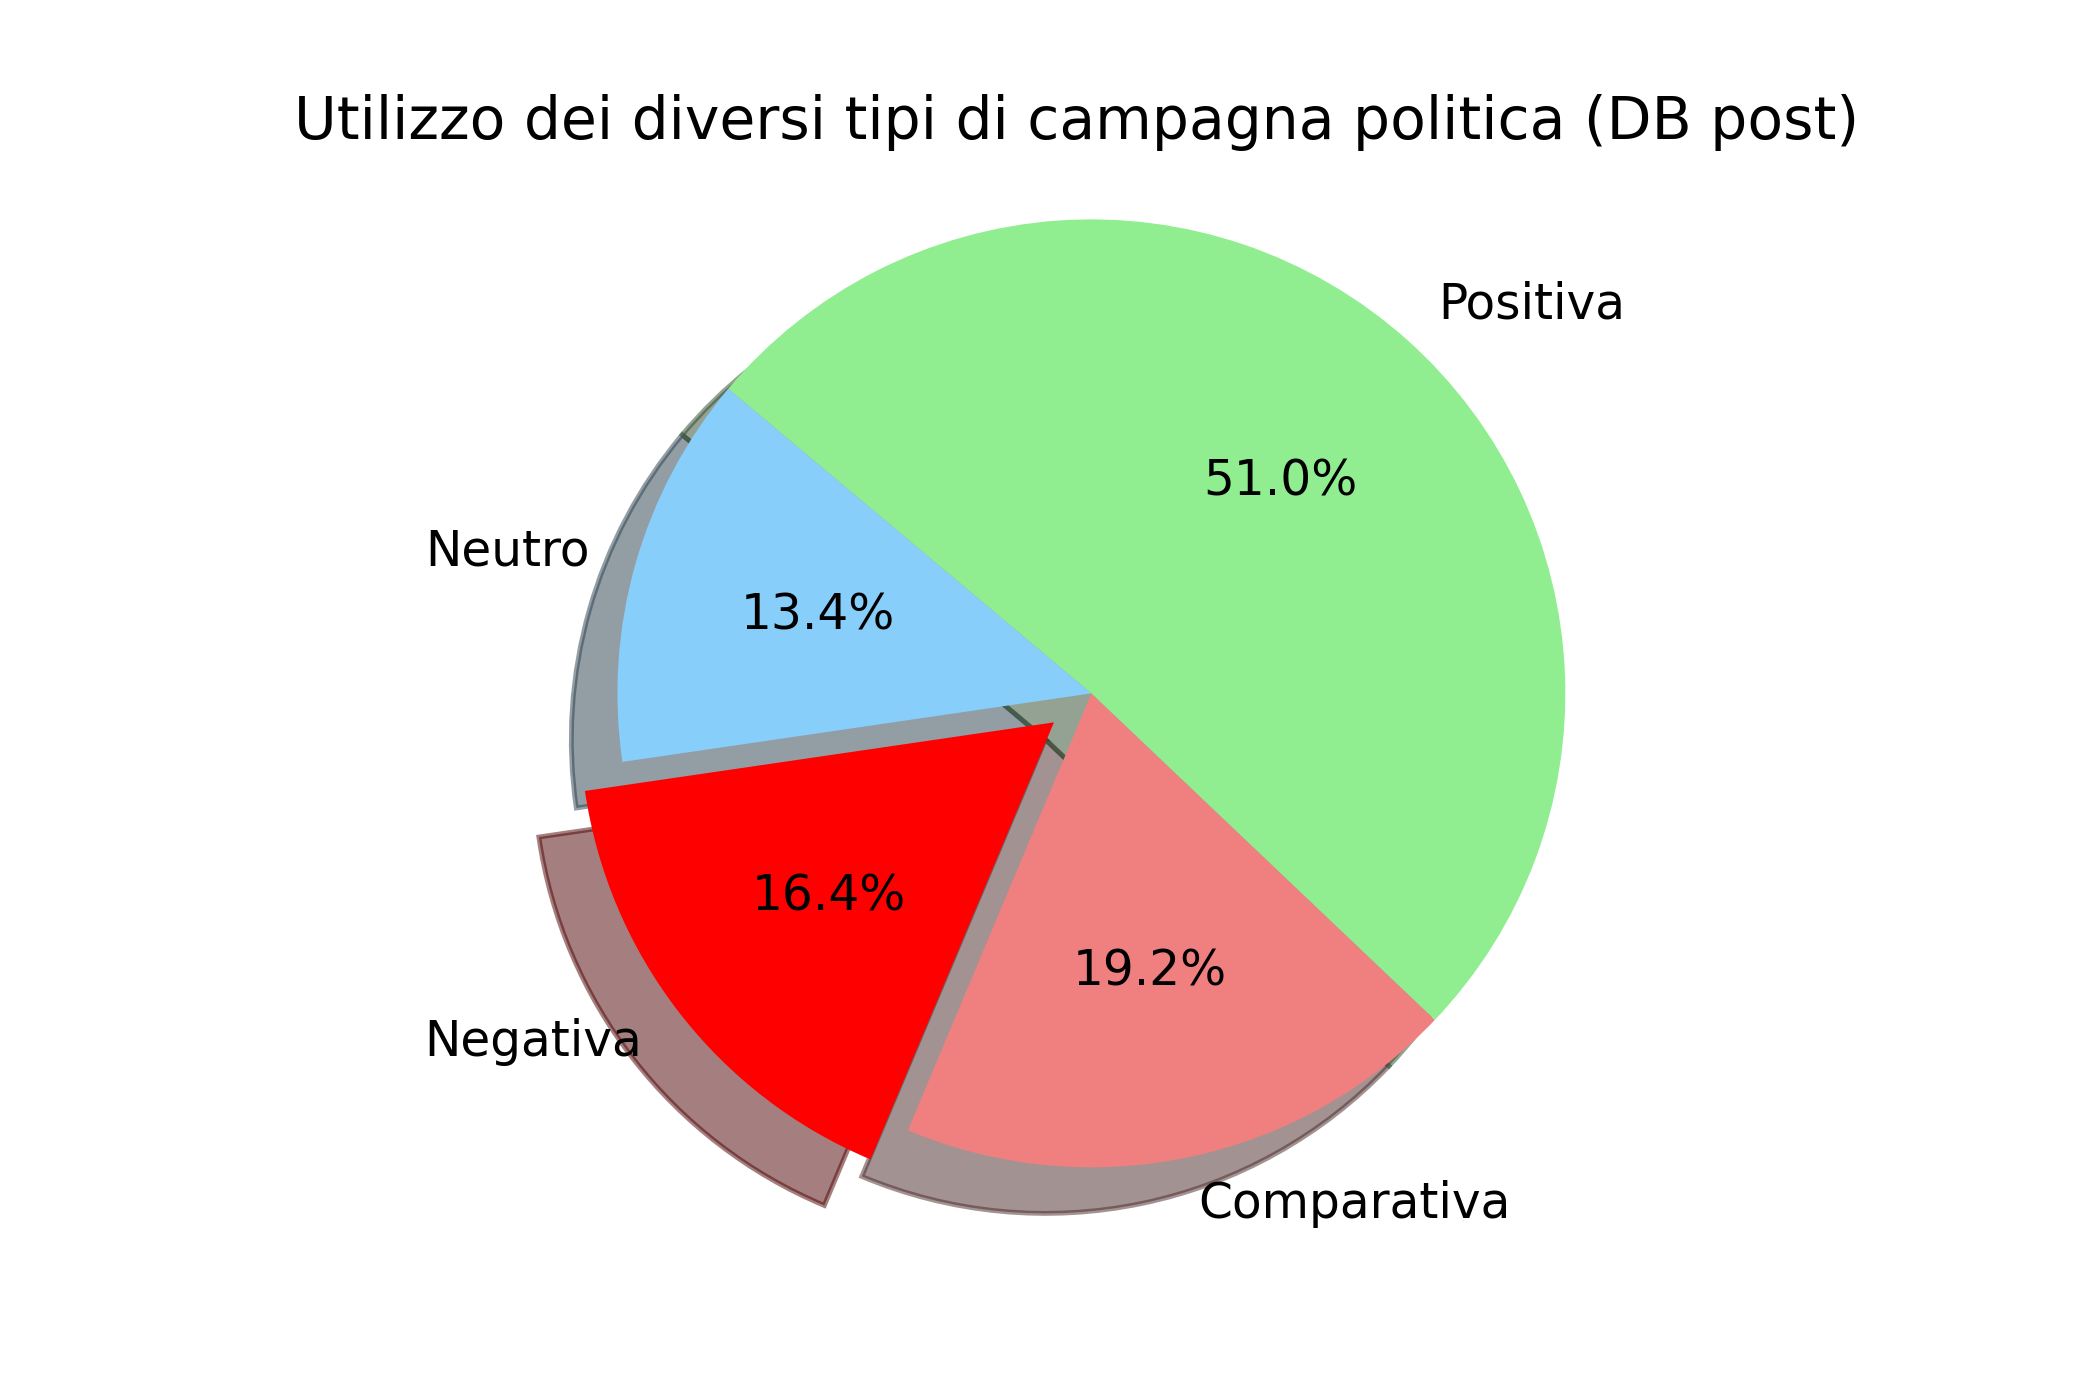
\includegraphics[width=\textwidth]{figures/tipoDiCampagnapie}
	\caption{L'utilizzo dei diversi tipi di campagna politica sul totale dei post e tweet dei politici.}
	\label{fig:campagna}
\end{figure}

Questi dati rimangono difficilmente confrontabili con quelli di studi precedenti per almeno due motivi: da una parte ogni ricerca analizza solo una parte dei canali informativi all'interno dei quali viene fatta propaganda elettorale e sappiamo che i livelli di odio possono cambiare in base al linguaggio comunicativo dettato dal medium; dall'altra parte l'applicazione della definizione di \textit{negative campaign}, benchè nella sua accezione direzionale risulti chiara e sgombra da fraintendimenti, è stata declinata con diversi tipi di sottocategorie. È importante aggiungere anche il fatto che i dati relativi ad elezioni nazionali e non europee risultano difficilmente confrontabili a causa delle differenze di coinvolgimento dei diversi tipi di elettorato.

Per quanto poco significativo, il confronto con gli studi relativi alle campagne elettorali degli Stati Uniti sembra indicare, comunque, una minore presenza di campagne negative in Italia. Guardando ad articoli che analizzano questo tipo di percentuali negli ultimi decenni \citep{geer2012} \citep{druckman2010} \citep{media2018}, possiamo dire che i dati mostrano risultati più vicini a quelli riscontrati in europa \citep{walter2014}, in particolare in uno scenario politico non bipartitico \citep{papp2018}, come registrato in altri studi che prendono in considerazione l’Italia \citep{ceron2016} \citep{seddone2019} citati nel capitolo "\nameref{chap:negative}".

\subsection{Ip.2: Negative campaign: chi lo usa?}
Le percentuali dei vari tipi di campagna politica non risultano omogenee attraverso tutto l'arco elettorale. Dai dati raccolti emergono delle percentuali molto diverse a seconda del partito analizzato. Nel primo grafico di questo paragrafo  [Fig. \ref{fig:partiti}] possiamo osservare i principali quattro partiti candidati alle elezioni e le loro diverse strategie comunicative. Nell'in-sieme, essi  rappresentano il 75\% di tutti i post e tweet raccolti. Risulta che PD e Fratelli d'Italia sono i partiti che usano maggiormente, in percentuale sui post analizzati, rispettivamente la campagna negativa e quella comparativa. Il partito che al contrario fa riscontrare una percentuale largamente maggiore di campagna positiva risulta essere il Movimento 5 Stelle con oltre il 71\% di utilizzo di post di questo tipo tra i suoi candidati alle europee.
\begin{figure}
	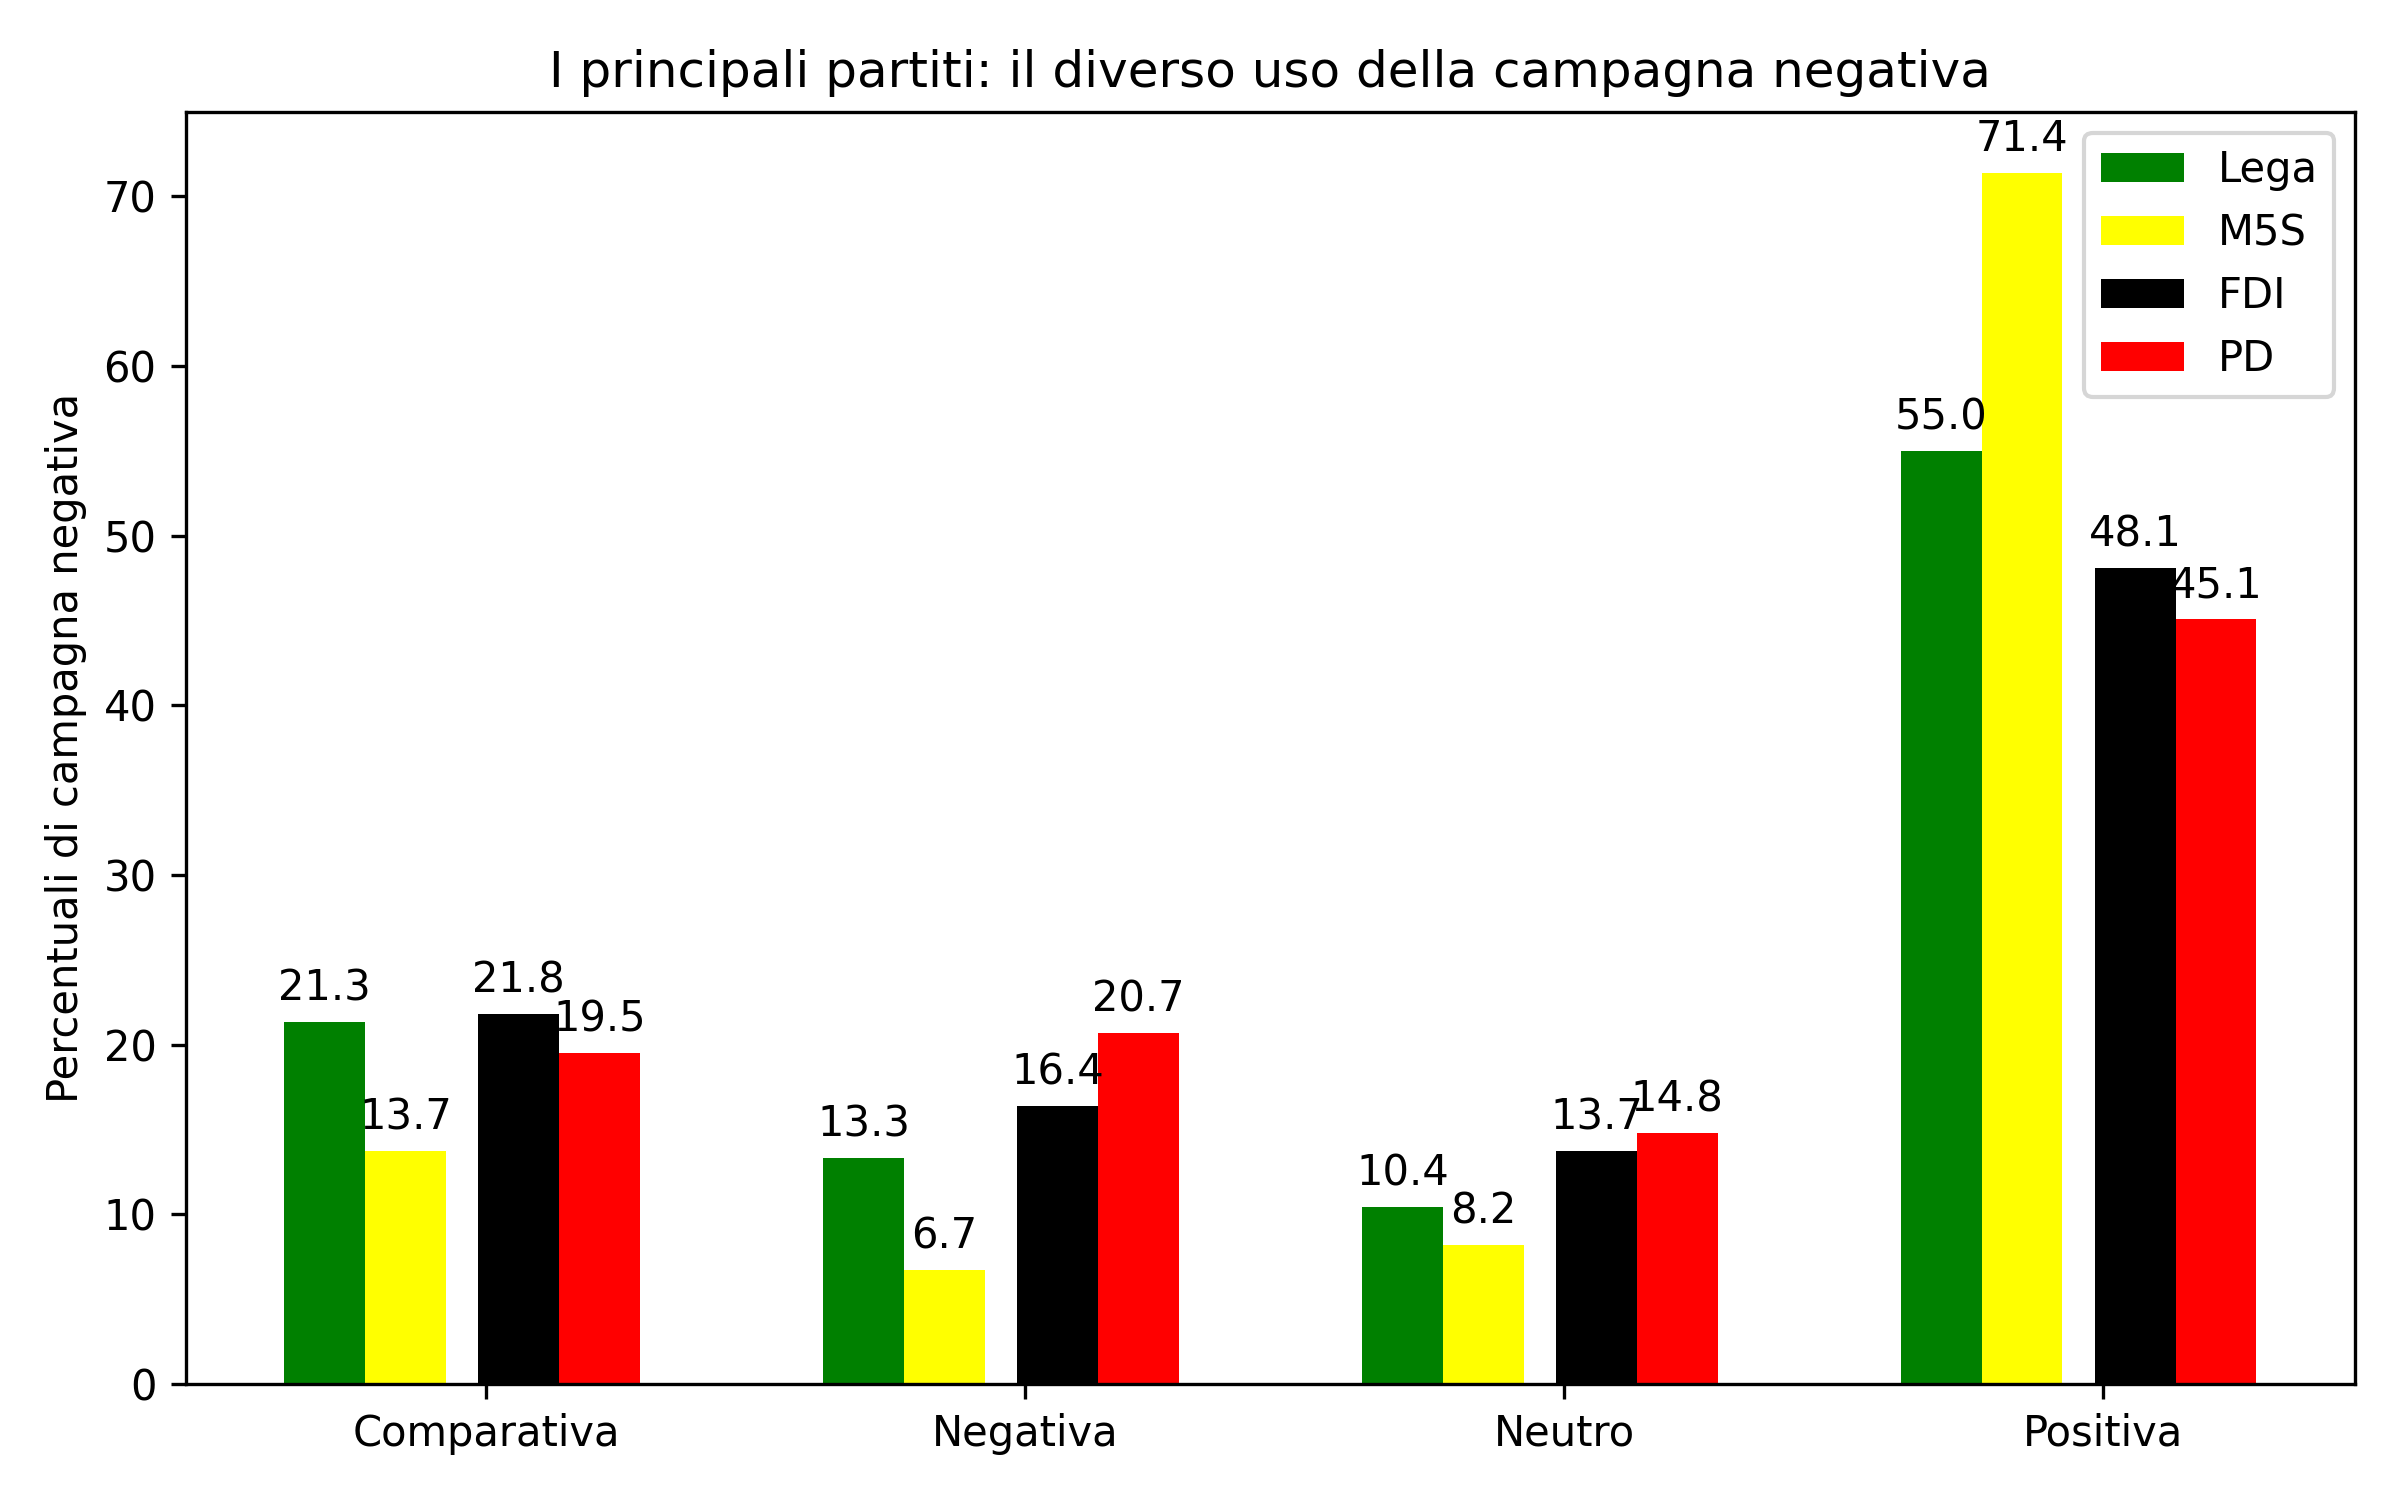
\includegraphics[width=\textwidth]{figures/partiti}
	\caption{I quattro principali partiti e il loro utilizzo dei tipi di campagna politica a confronto. Le percentuali di tipo di campagna per ogni partito}
	\label{fig:partiti}
\end{figure}

Nella tabella riportata di seguito [Fig. \ref{fig:partiti2}] possiamo vedere le percentuali di tutti i partiti a confronto, anche quelli minori non presenti nel grafico precedente. Emerge che anche formazioni minori, che rappresentano poco meno del 5\% dei post-tweet analizzati (+Europa e La Sinistra), hanno proposto confronti e attacchi a rivali con una frequenza maggiore rispetto alla media di tutti i partiti considerati contemporaneamente. La Sinistra risulta essere il più propenso a questo tipo di comunicazione, con valori intorno al 30\%, sia per la campagna comparativa che per quella negativa.
\begin{figure}
	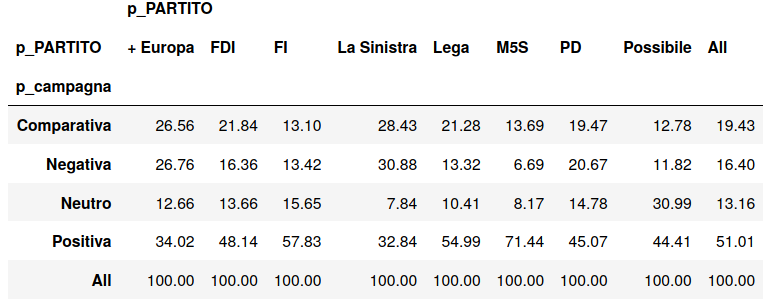
\includegraphics[width=\textwidth]{figures/partiticampagna}
	\caption{Le percentuali di tipi di campagna utilizzati da tutti i partiti.}
	\label{fig:partiti2}
\end{figure}

Sembra interessante, quindi, chiedersi quale sia il motivo alla base di differenze così marcate. A tal fine, sono state prese in considerazione due ipotesi. La prima è che l'utilizzo di campagne negative e comparative sia dovuto prevalentemente alla posizione istituzionale ricoperta dal partito, cioè se esso sia al governo oppure all'opposizione a livello nazionale.

Benché stiamo analizzando la campagna per le elezioni europee, come detto anche nel capitolo "\nameref{chap:metodologia}", risultano comunque pochissimi riferimenti a ciò che è stato fatto dei rispettivi partiti nella legislazione europea appena conclusa; ci si è piuttosto concentrati sull'idea futura di Europa e sulla politica interna \citep{seddone2019}. Facciamo quindi riferimento agli schieramenti in carica (Lega e M5S) o meno nel parlamento nazionale al momento della campagna elettorale. Raggruppati i partiti in due gruppi, le  differenze nell'utilizzo dei tipi di campagna vengono analizzate tramite test di chi-quadro. Questo test verrà poi confrontato con un secondo test in cui il raggruppamento avverrà in base all'appartenenza del partito a posizioni di sinistra o di destra.

Come vediamo con il test successivo, benché la campagna comparativa risulti utilizzata in egual misura dai due schieramenti divisi in base al loro ruolo istituzionale, nella campagna comparativa e in quella positiva le percentuali risultano opposte tra i due gruppi [Fig. \ref{fig:governo}]. Chi è al governo utilizza molti più messaggi in cui racconta le sue proposte in positivo e parla degli obiettivi raggiunti negli ultimi mesi. Chi è all'opposizione cerca di screditare gli avversari con messaggi negativi, si potrebbe suppore che lo faccia per guadagnare visibilità sui media.
\begin{figure}
	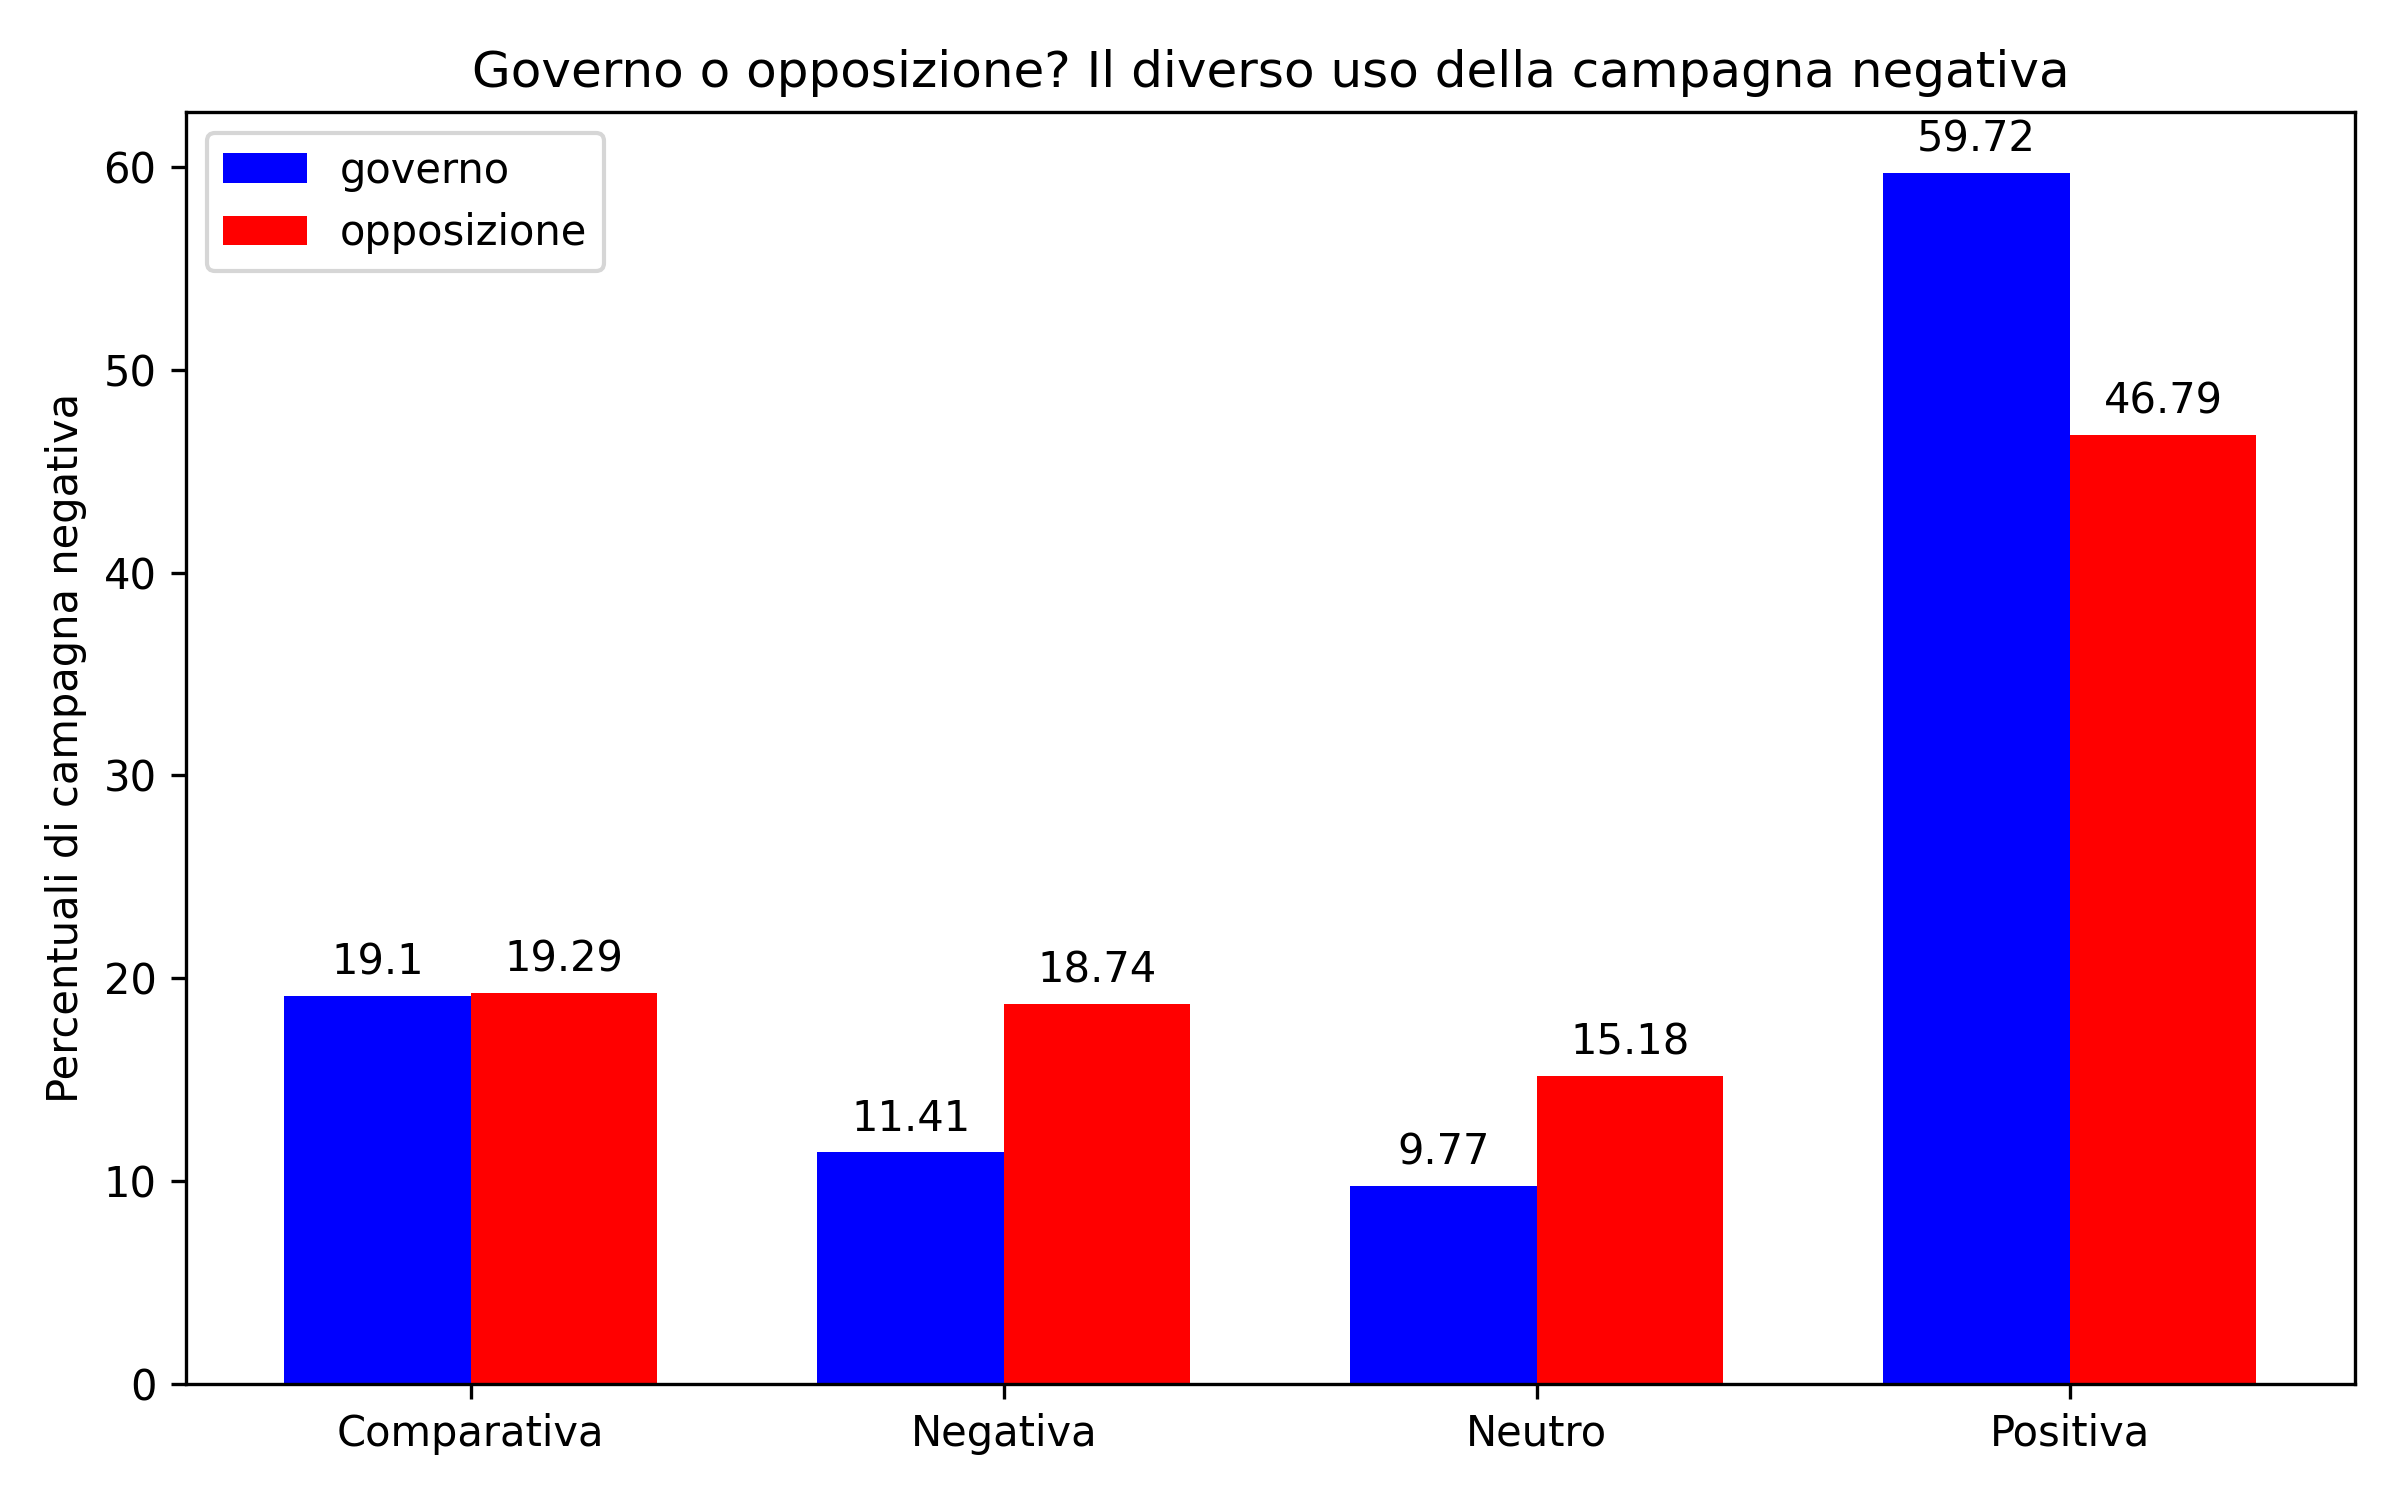
\includegraphics[width=\textwidth]{figures/governo}
	\caption{Le percentuali di tipi di campagna utilizzati dai partiti raggruppati in base alla posizione istituzionale (governo vs opposizione).}
	\label{fig:governo}
\end{figure}
%[Fig. \ref{fig:chigoverno}]
%  
%\begin{figure}
%    \centering
%    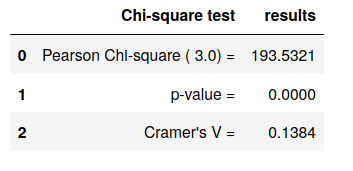
\includegraphics[width=0.5\textwidth]{figures/chigoverno}
%    \caption{Test di Chi Quadro relativo alle frequenze dei diversi tipi di campagna politica per i partiti raggruppati in base alla posizione istituzionale (governo vs opposizione).}
%    \label{fig:chigoverno}
%\end{figure}

Effettuando un test di chi quadro per verificare la significatività di queste differenze riscontrate , i risultati confermano l'ipotesi: $\chi^{2}$ (7, N = 10103) = 193.532, p = 0.0000. Data l'alta numerosità del campione, interessante il dato del chi-quadro di Pearson che mostra una differenza molto elevata tra le frequenze sottoposte al test.

Sondando la seconda ipotesi, raggruppando cioè i partiti in base allo schieramento ideologico a cui appartengono, otteniamo dei risultati che confermano delle differenze tra destra e sinistra, ma meno marcate rispetto al test precedente [Fig. \ref{fig:destra}]. Interessante il fatto che la campagna comparativa rimanga invariata nelle sue percentuali, dimostrando come ci sia un'effettiva differenza con la campagna negativa, le cui percentuali invece variano leggermente.
\begin{figure}
	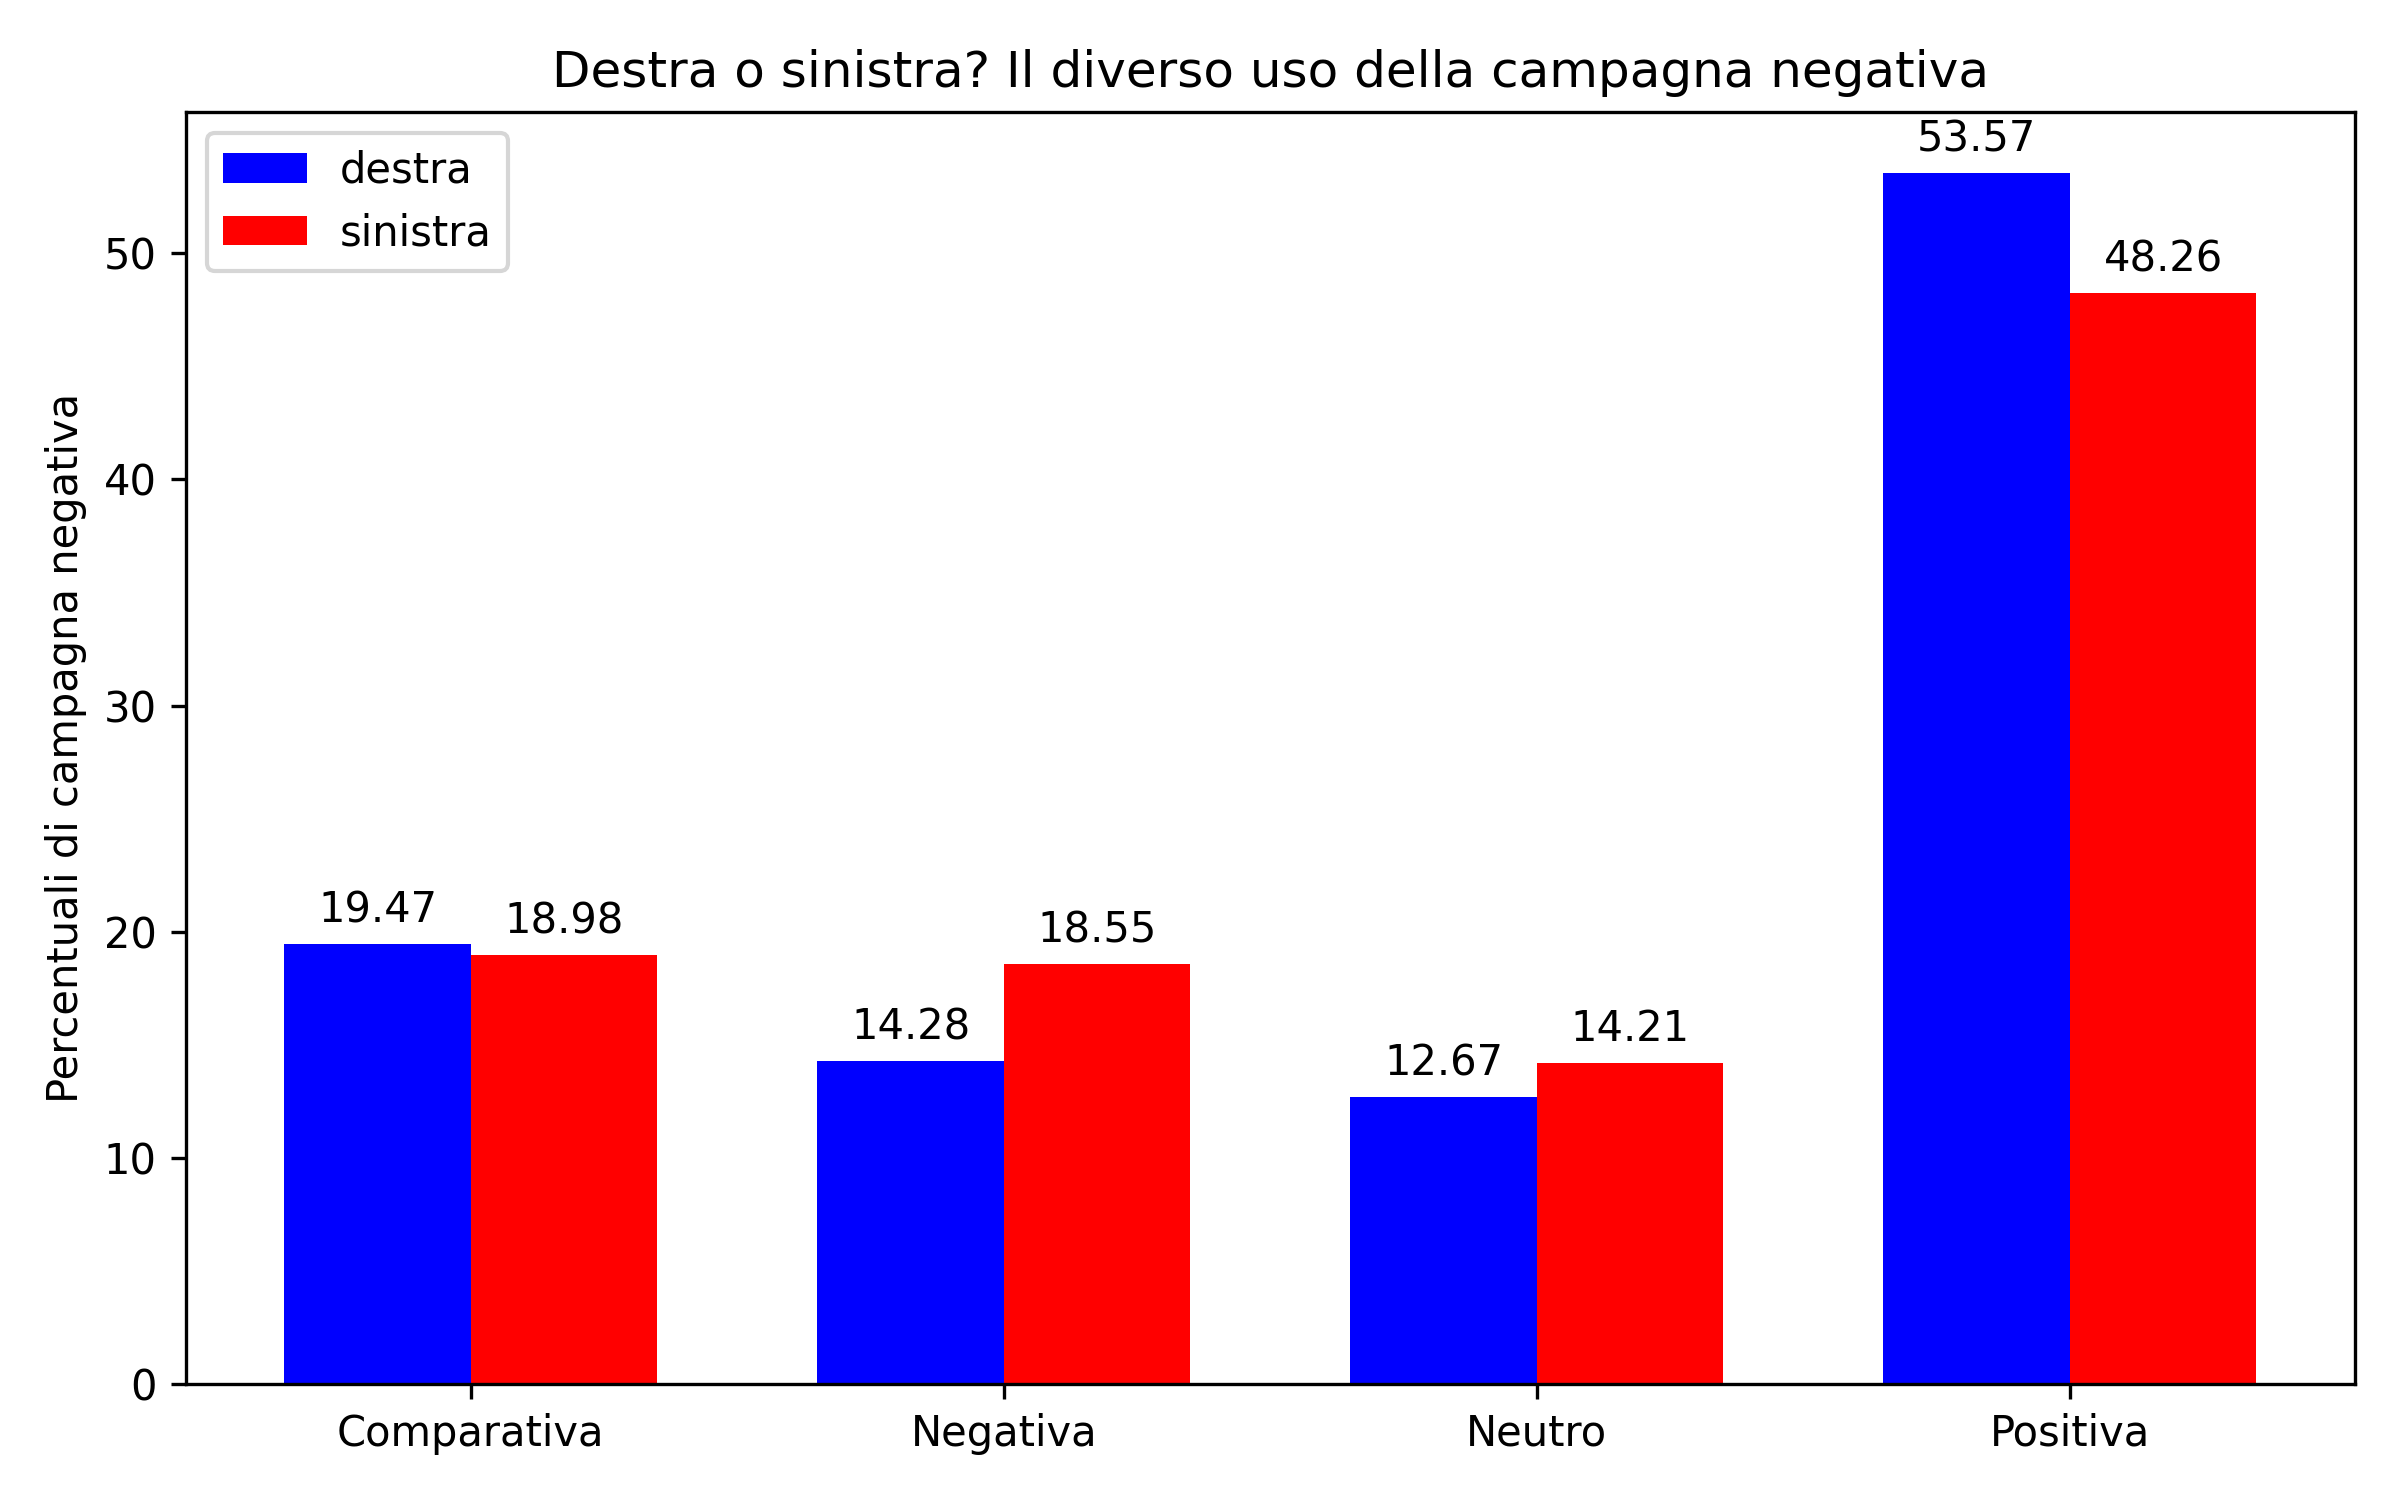
\includegraphics[width=\textwidth]{figures/destra}
	\caption{Le percentuali di tipi di campagna utilizzati dai partiti raggruppati in base alla posizioni di governo (destra vs sinistra).}
	\label{fig:destra}
\end{figure}

%[Fig. \ref{fig:chidestra}]
%\begin{figure}
%    \centering
%    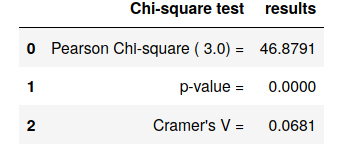
\includegraphics[width=0.5\textwidth]{figures/chidestra}
%    \caption{}
%    \label{fig:chidestra}
%\end{figure}

Effettuando un test di chi-quadro anche in questo caso  i risultati mostrano un p-value significativo allo stesso modo, ma con un valore del test di Pearson minore: $\chi^{2}$ (7, N = 10103) = 46.8791, p = 0.0000. Possiamo quindi affermare che questo tipo di ipotesi risulta meno utile per spiegare cosa spinge a utilizzare una strategia comunicativa rispetto ad un’altra.

\subsubsection{Movimento 5 Stelle: sinistra o destra?}
Per questo test il Movimento 5 Stelle è stato classificato come un partito di sinistra, tuttavia la categorizzazione di questo specifico partito rimane una questione aperta. Alcune posizioni (come quelle sull'ambiente) possono essere sicuramente assimilate a quelle della sinistra classica, sulla questione dell'immigrazione, invece, soprattutto nel periodo di governo con la Lega, le posizioni sono state più tendenti a quelle della destra populista. Il problema alla base di questo dilemma rimane il fatto che i rappresentanti del partito stesso hanno sempre preferito porsi in opposizione a tutta la "casta" rifiutando esplicitamente di essere inseriti in uno dei due schieramenti classici, mirando ad  essere votati dagli elettori di entrambi e finendo per governare prima con la destra e poi con la sinistra. Provando a spostare il Movimento nello schieramento di destra, comunque, le considerazioni generali rimangono invariate poiché il test di chi-quadro, anche in questo caso, rileva minori differenze nell'utilizzo del \textit{negative campaign} rispetto alla teoria della posizione di governo: $\chi^{2}$ (7, N = 10103) = 70.8986, p = 0.0000.

In conclusione, l'ipotesi riportata in diversi articoli della letteratura sul genere \citep{hansen2008} \citep{druckman2010} \citep{walter2014} \citep{curini2010}, secondo cui il \textit{negative campaign} risulta prevalente nei partiti che devono conquistare il potere rispetto a quelli che devono mantenerlo poiché si trovano già al governo, risulta confermata e avvalorata da confronti con altre ipotesi alternative che, seppur in grado di evidenziare alcune differenze, risultano meno efficaci.

\subsection{Ip.3: Il \textit{negative campaign} in relazione al tipo di social network}
A seguito delle riflessioni contenute nei capitoli precedenti sui due social presi in considerazione, risulta interessante indagare come la comunicazione politica cambi a seconda del medium utilizzato. Comparando i valori generali attraverso tutti i partiti [Fig. \ref{fig:site}] risulta effettivamente che Facebook è maggiormente utilizzato per campagne comparative e positive che naturalmente necessitano più spazio per essere argomentate. Le campagne negative invece risultano più utilizzate sulla piattaforma dei cinguettii, che sembra quindi prediligere attacchi diretti piuttosto che confronti tra i propri temi e quelli degli avversari.
\begin{figure}
	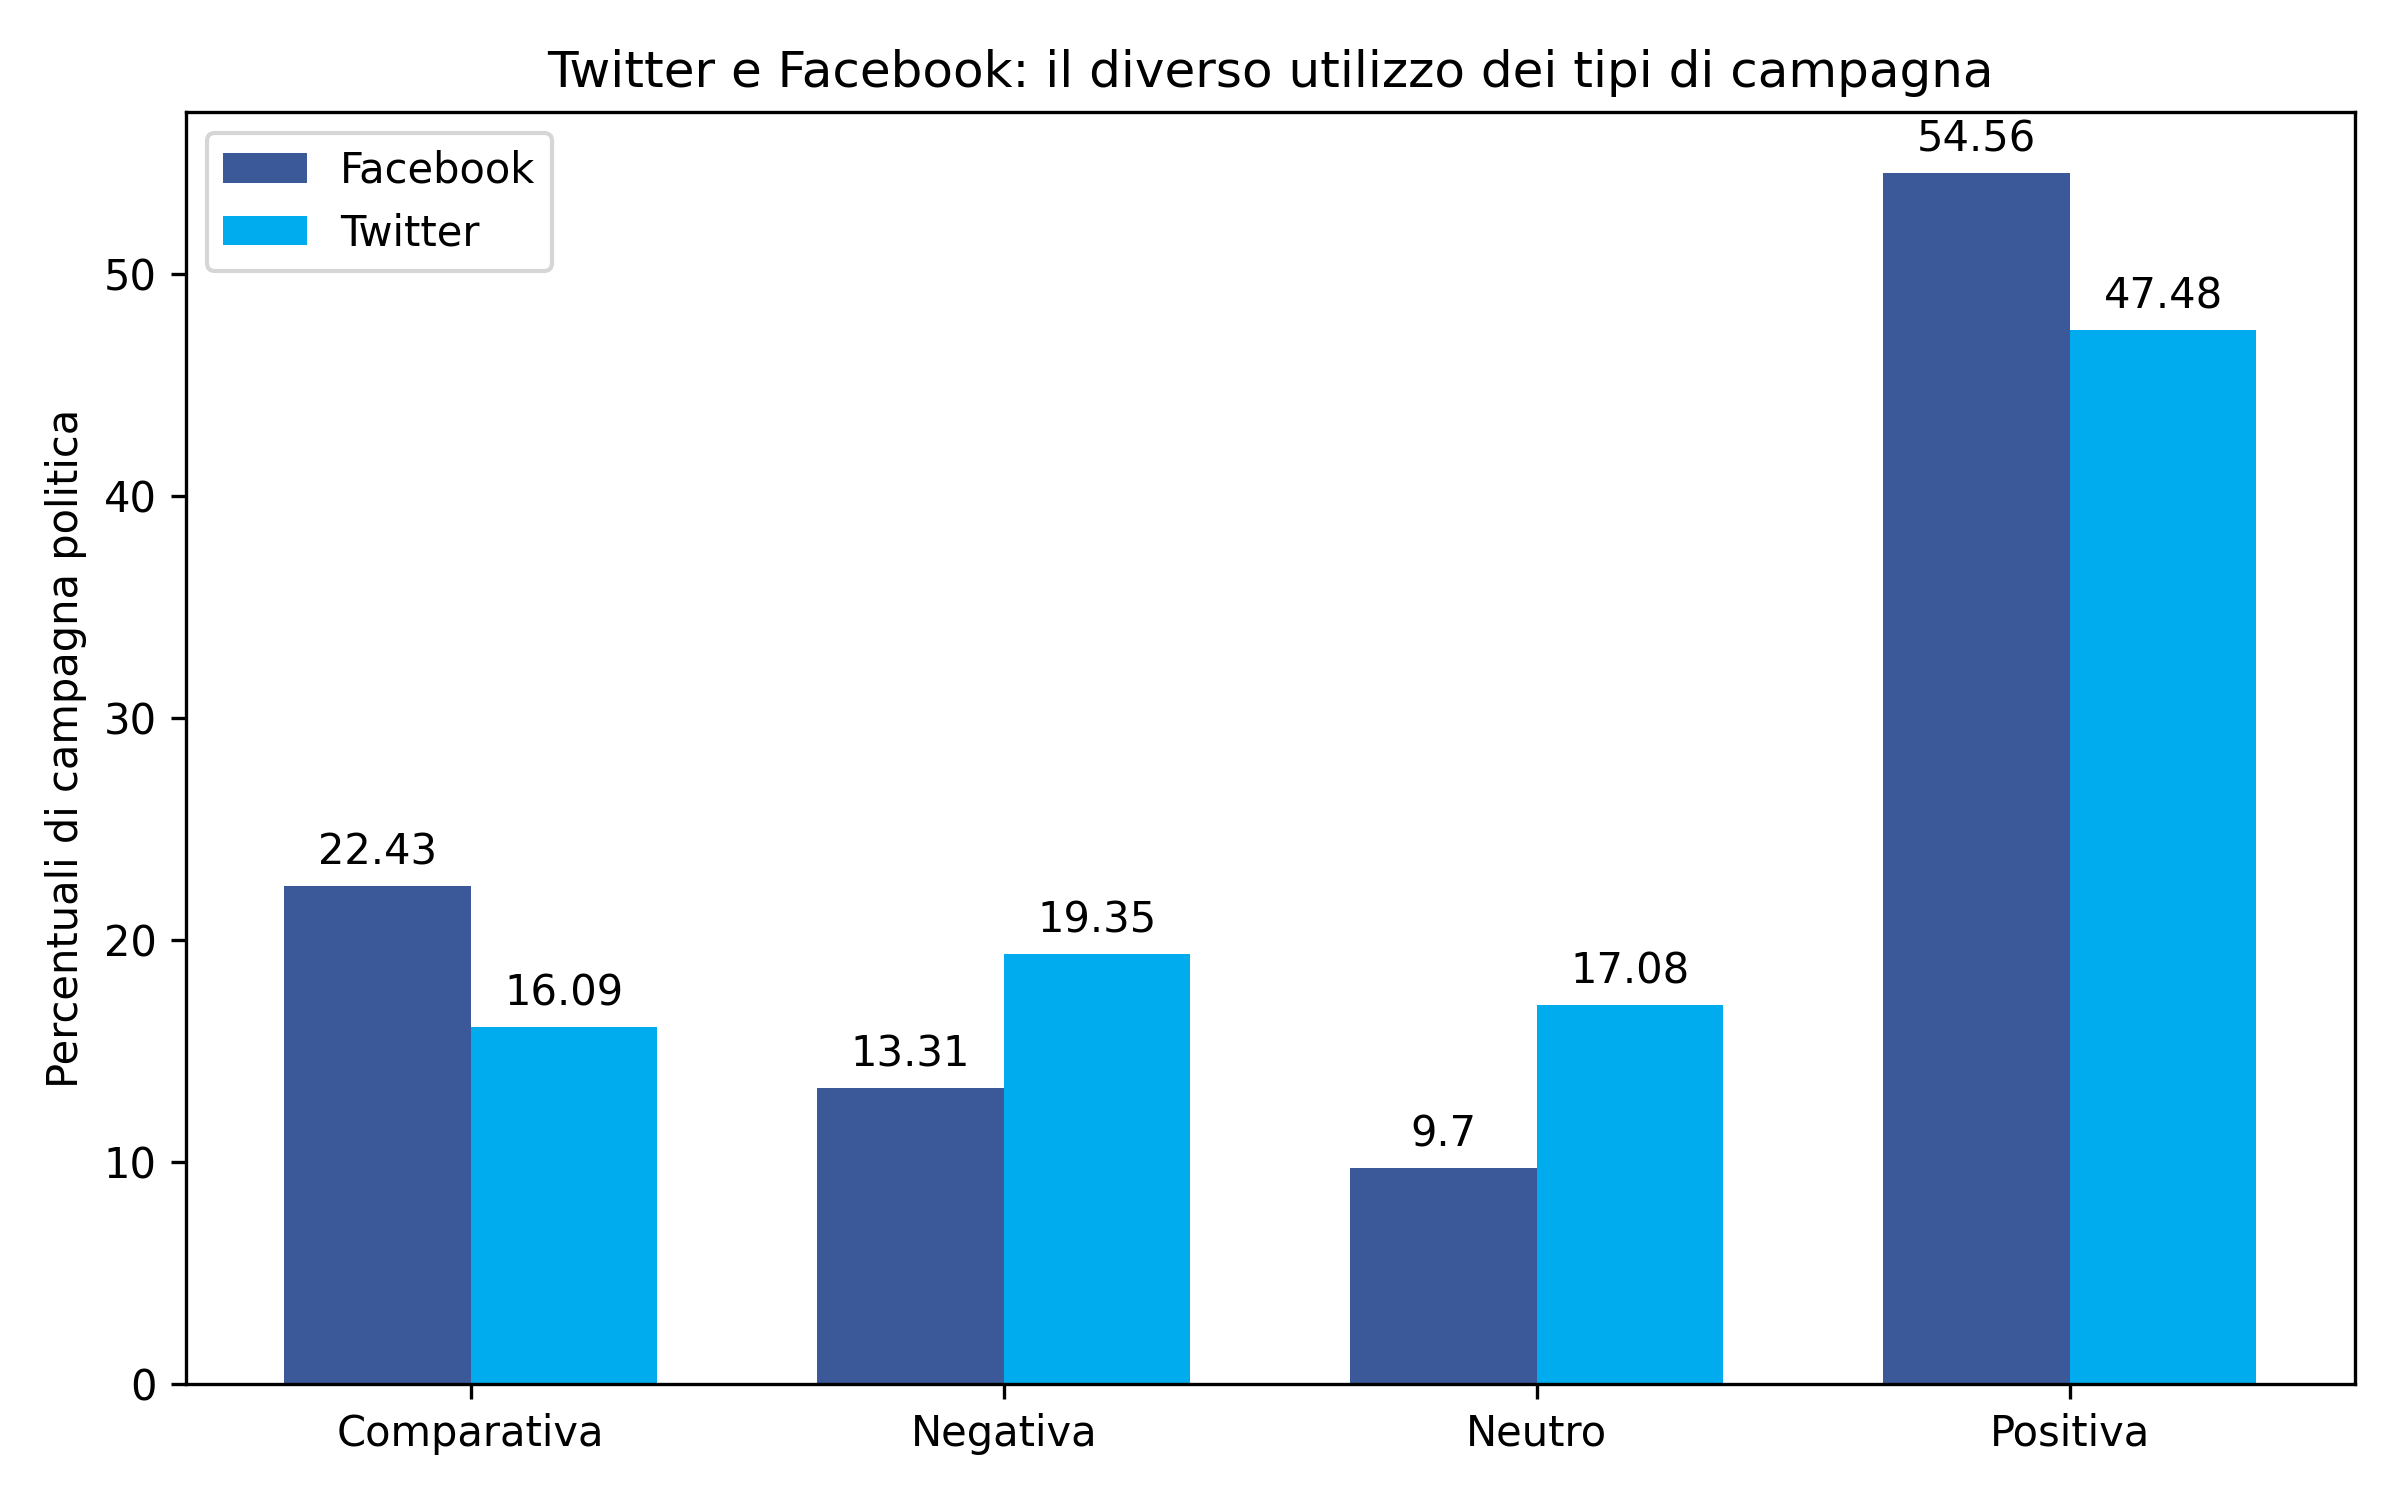
\includegraphics[width=\textwidth]{figures/site}
	\caption{Le percentuali di tipi di campagna in base alla piattaforma sul quale sono stati postati.}
	\label{fig:site}
\end{figure}

Anche verificando la lunghezza media del testo dei post dei vari tipi di campagna su  entrambe le piattaforme risulta che in quelle comparative vengano utilizzati più caratteri ris-petto alle negative (Comparativa = 65.0, Negativa = 40.1). E questo fenomeno persiste anche confrontando le lunghezze medie di questi tipi di campagna sui social presi singolarmente: su Facebook  quella comparativa ha una media di 86.40 caratteri, la negativa di 53.04 (N = 5002); su Twitter invece la comparativa è mediamente di 35.55, la negativa di 31.34 (N = 5101).

Analizzando l’utilizzo comparato di Facebook [Fig. \ref{fig:partitifb}] e Twitter [Fig. \ref{fig:partititw}] da parte dei  quattro principali partiti (Lega, M5S, FDI, PD) presi singolarmente e poi la differenza tra le percentuali dei diversi tipi di campagna tra le due piattaforme [Fig. \ref{fig:partitic}], emergono le stesse indicazioni dell’analisi aggregata.\begin{figure}
	\centering
	\begin{minipage}{.5\textwidth}
		\centering
		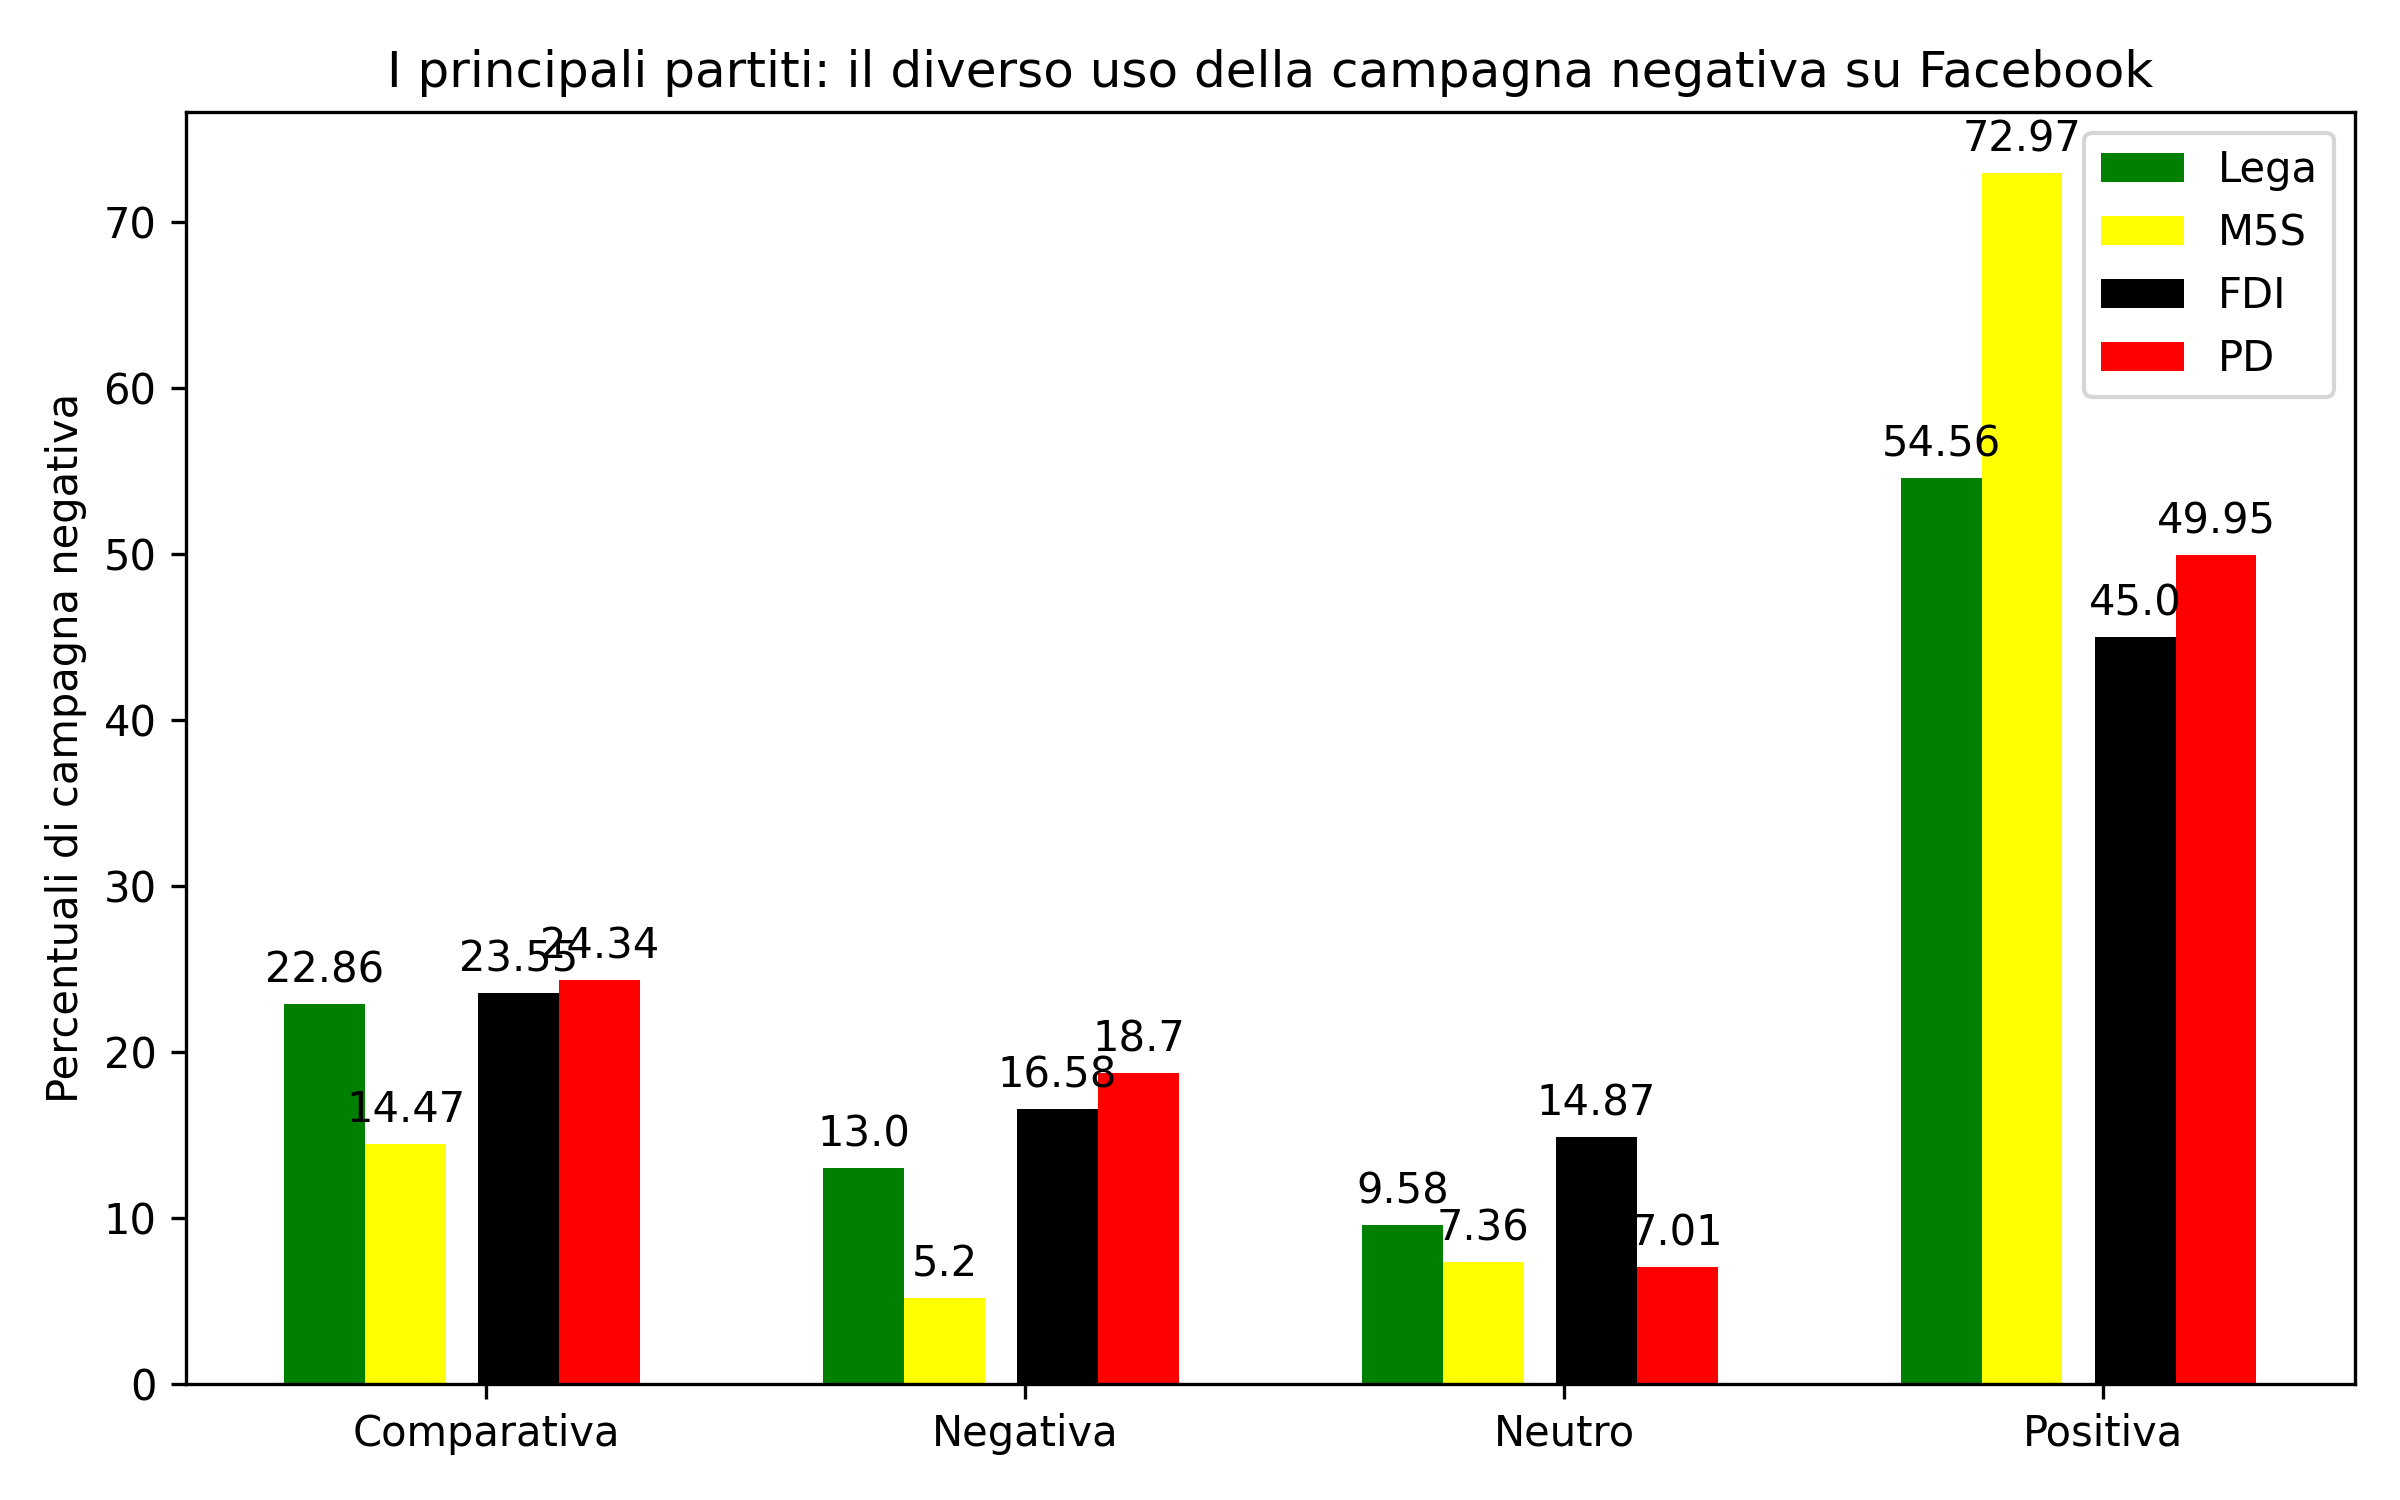
\includegraphics[width=\linewidth]{figures/partitifb}
		\captionof{figure}{I principali partiti a confronto: utilizzo dei vari tipi di campagna politica su Facebook.}
		\label{fig:partitifb}
	\end{minipage}%
	\begin{minipage}{.5\textwidth}
		\centering
		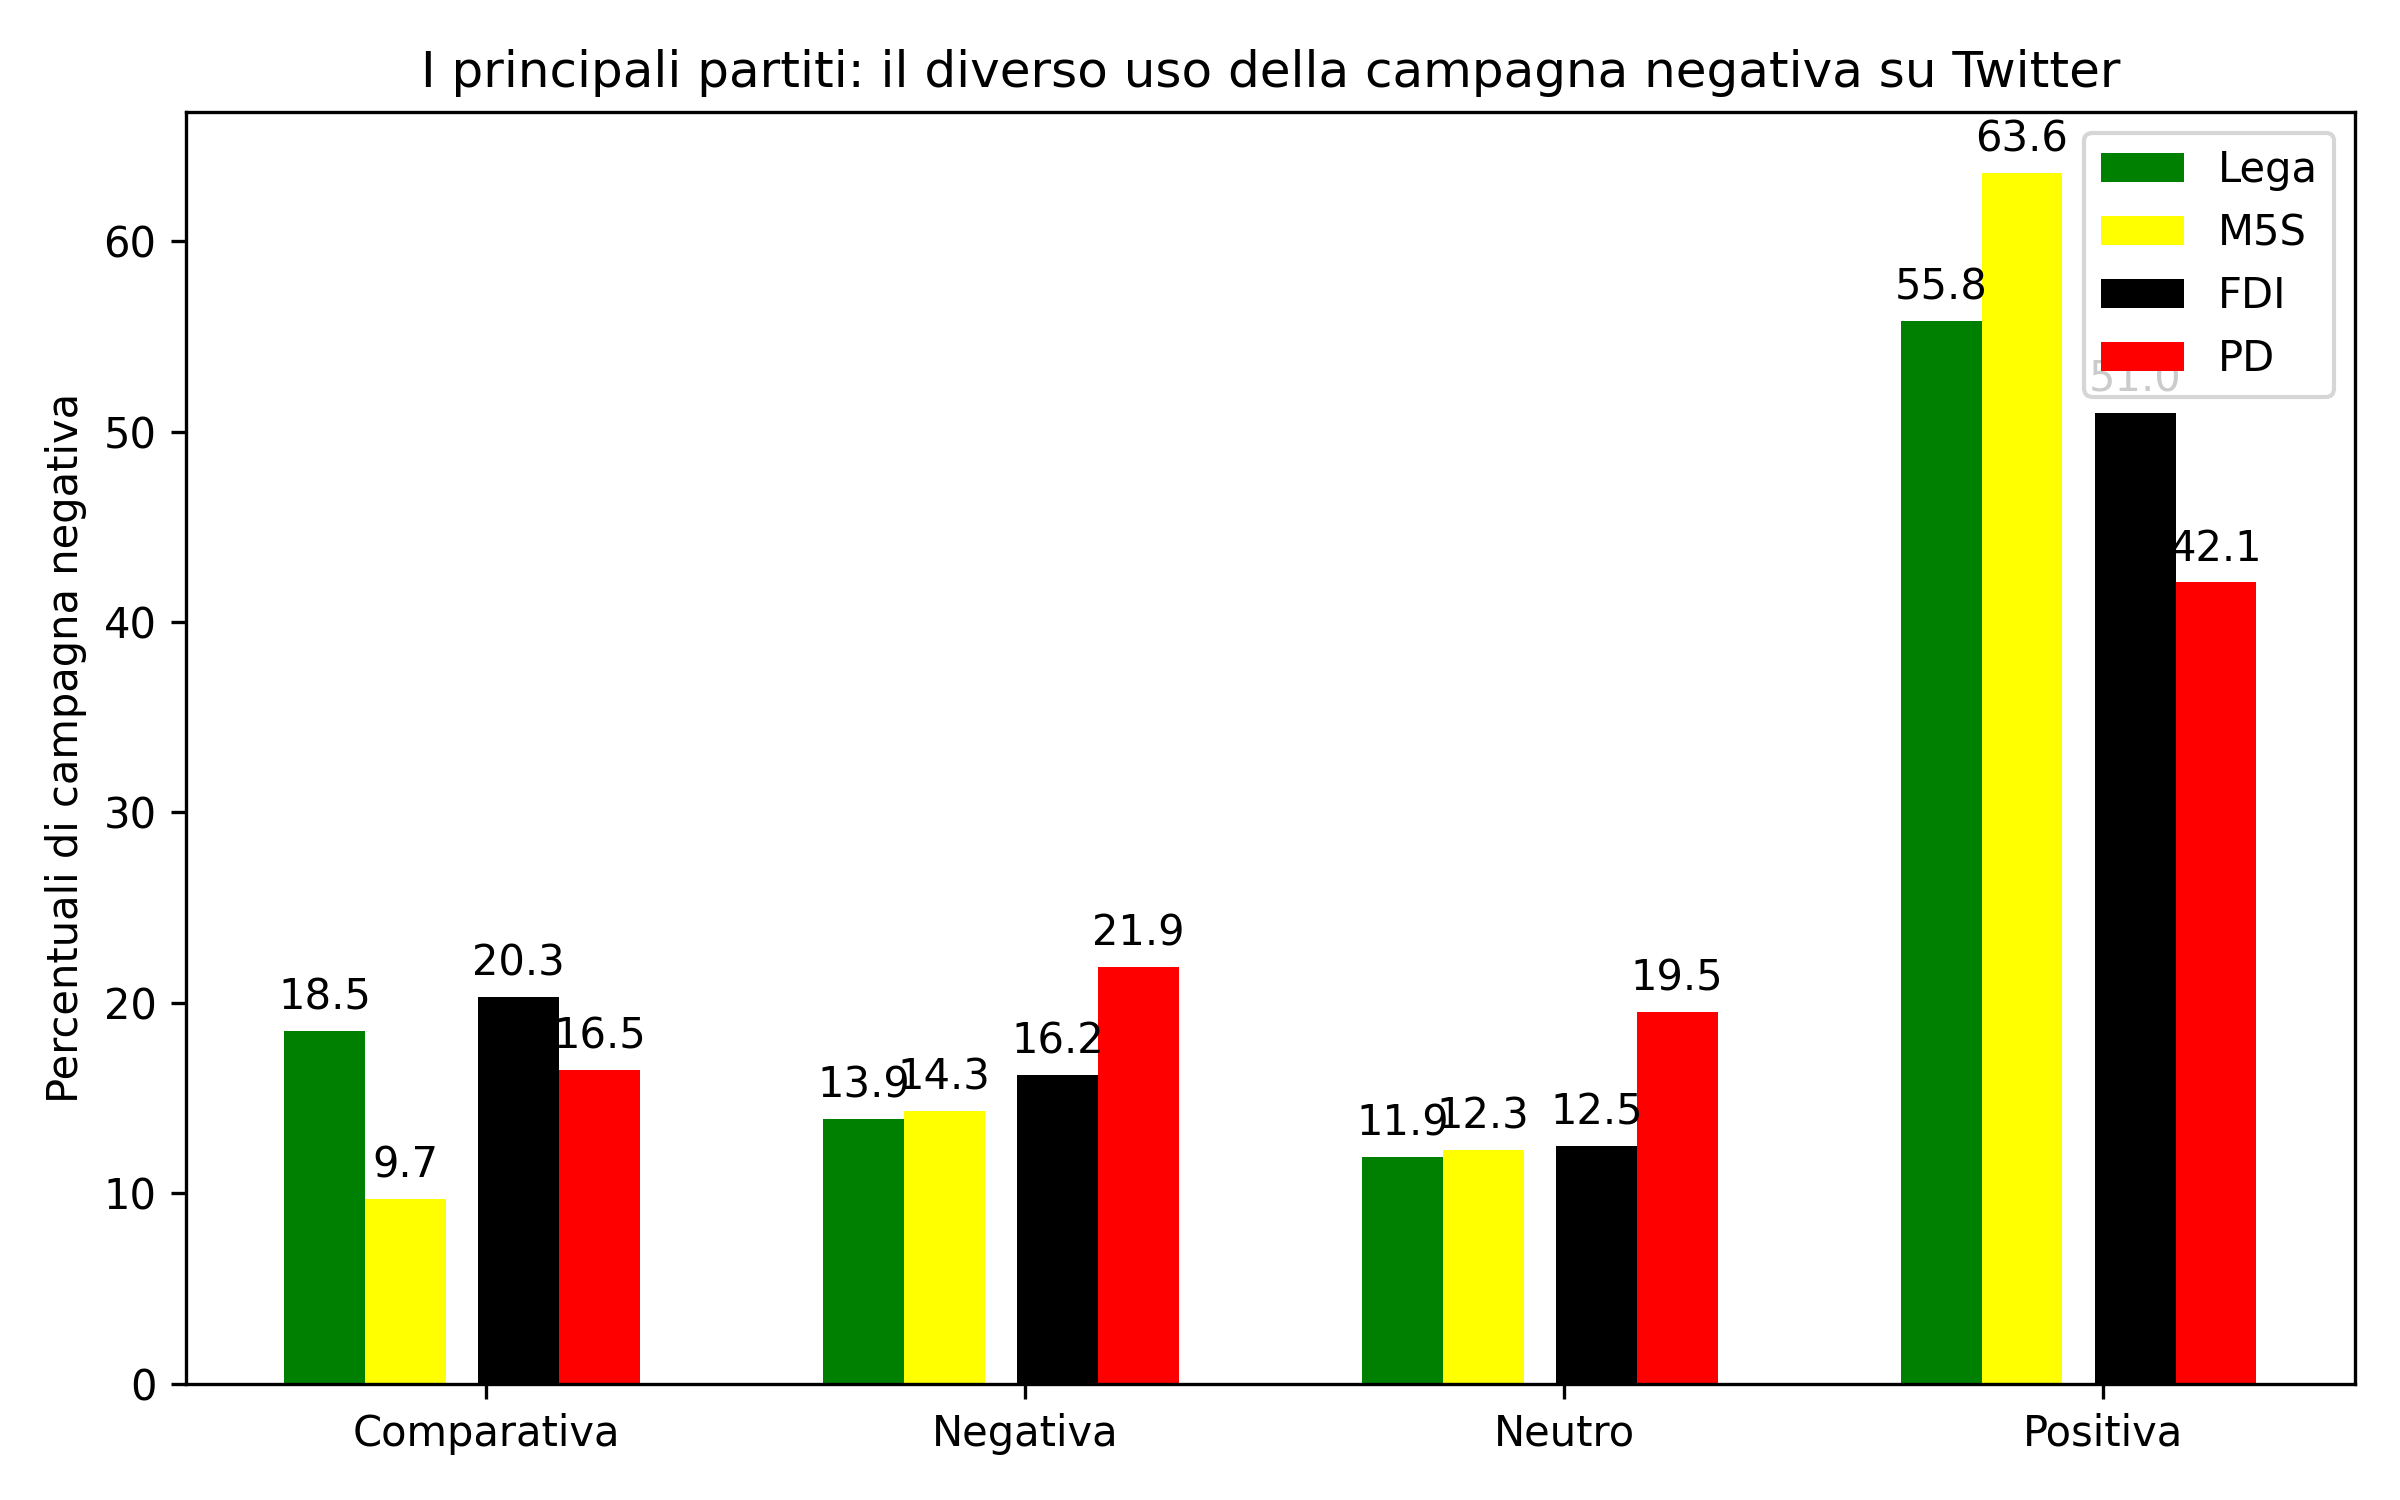
\includegraphics[width=\linewidth]{figures/partititw}
		\captionof{figure}{I principali partiti a confronto: utilizzo dei vari tipi di campagna politica su Twitter.}
		\label{fig:partititw}
	\end{minipage}
\end{figure}
\begin{figure}
	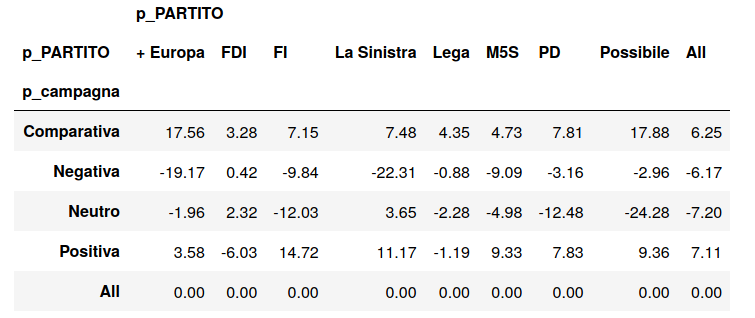
\includegraphics[width=\textwidth]{figures/partitic}
	\caption{Differenza tra le percentuali dei vari tipi di campagna politica per i singoli partiti: ai valori riscontrati su Facebook vengono sottratti quelli riscontrati su Twitter. A valori positivi corrisponde quindi una maggiore percentuale di utilizzo di un certo tipo di campagna su Facebook rispetto a Twitter.}
	\label{fig:partitic}
\end{figure}

Tutte le formazioni in campo prediligono Facebook per le comparazioni tra i propri temi e quelli degli avversari. A parte FDI e Lega (che presentano variazioni minime) tutti i partiti fanno riscontrare un aumento percentuale delle campagne negative su Twitter rispetto a Facebook.  Questo dato è più evidente nei due partiti minori che hanno utilizzato maggiormente questo tipo di campagna (+Europa e La Sinistra), in percentuale sul totale di post e tweet pubblicati, arrivando a un aumento di circa il 20\% nel passaggio da una piattaforma all’altra.

In conclusione: tutti i partiti, a seconda della piattaforma social utilizzata, fanno riscontrare percentuali diverse nelle tipologie di campagna proposta. Questa differenza sembra andare nella direzione di una maggiore negatività per Twitter e un maggiore utilizzo di messaggi comparativi su Facebook.  Le variazioni sono probabilmente collegate alla lunghezza media dei due tipi di messaggio, che essendo più lunghi per la campagna comparativa e più brevi per quella negativa, si conciliano meglio con le regole comunicative dei due diversi social. Il medium indirizza quindi le forme di attacco politico.

\subsection{Ip.4: Il \textit{negative campaign} contribuisce a far diventare virali i contenuti?}
Riprendendo la letteratura sul tema, si è deciso di testare la viralità dei vari tipi di campanga politica. 
Su Twitter, post comparativi e negativi hanno una media di \textit{likes} quasi doppia rispetto agli altri due tipi di campagna che non prevedono di citare avversari politici [Fig. \ref{fig:viralitatw}]. Anche per quanto riguarda le risposte ai tweet e la ricondivisione degli stessi, i valori sono addirittura più che doppi per la campagna comparativa e almeno un 30\% più elevati per quella negativa.

Su Facebook invece, i risultati sono meno  univoci. Senza considerare i post neutri che fanno riscontrare il valore più elevato di likes in media, ma che, appunto, non hanno argomento politico e andrebbero analizzati uno per uno per capire le ragioni di tanto apprezzamento, i post comparativi fanno registrare una media più elevata nel numero di likes, seguiti da quelli positivi ed infine da quelli negativi.  [Fig. \ref{fig:viralitafb}]. Le statistiche di ricondivisione e risposte però, anche su questo social, osservano mediamente un  30\% percento in più circa nei casi in cui vengono citati gli avversari rispetto a quando non lo sono.
\begin{figure}
	\centering
	\begin{minipage}{.5\textwidth}
		\centering
		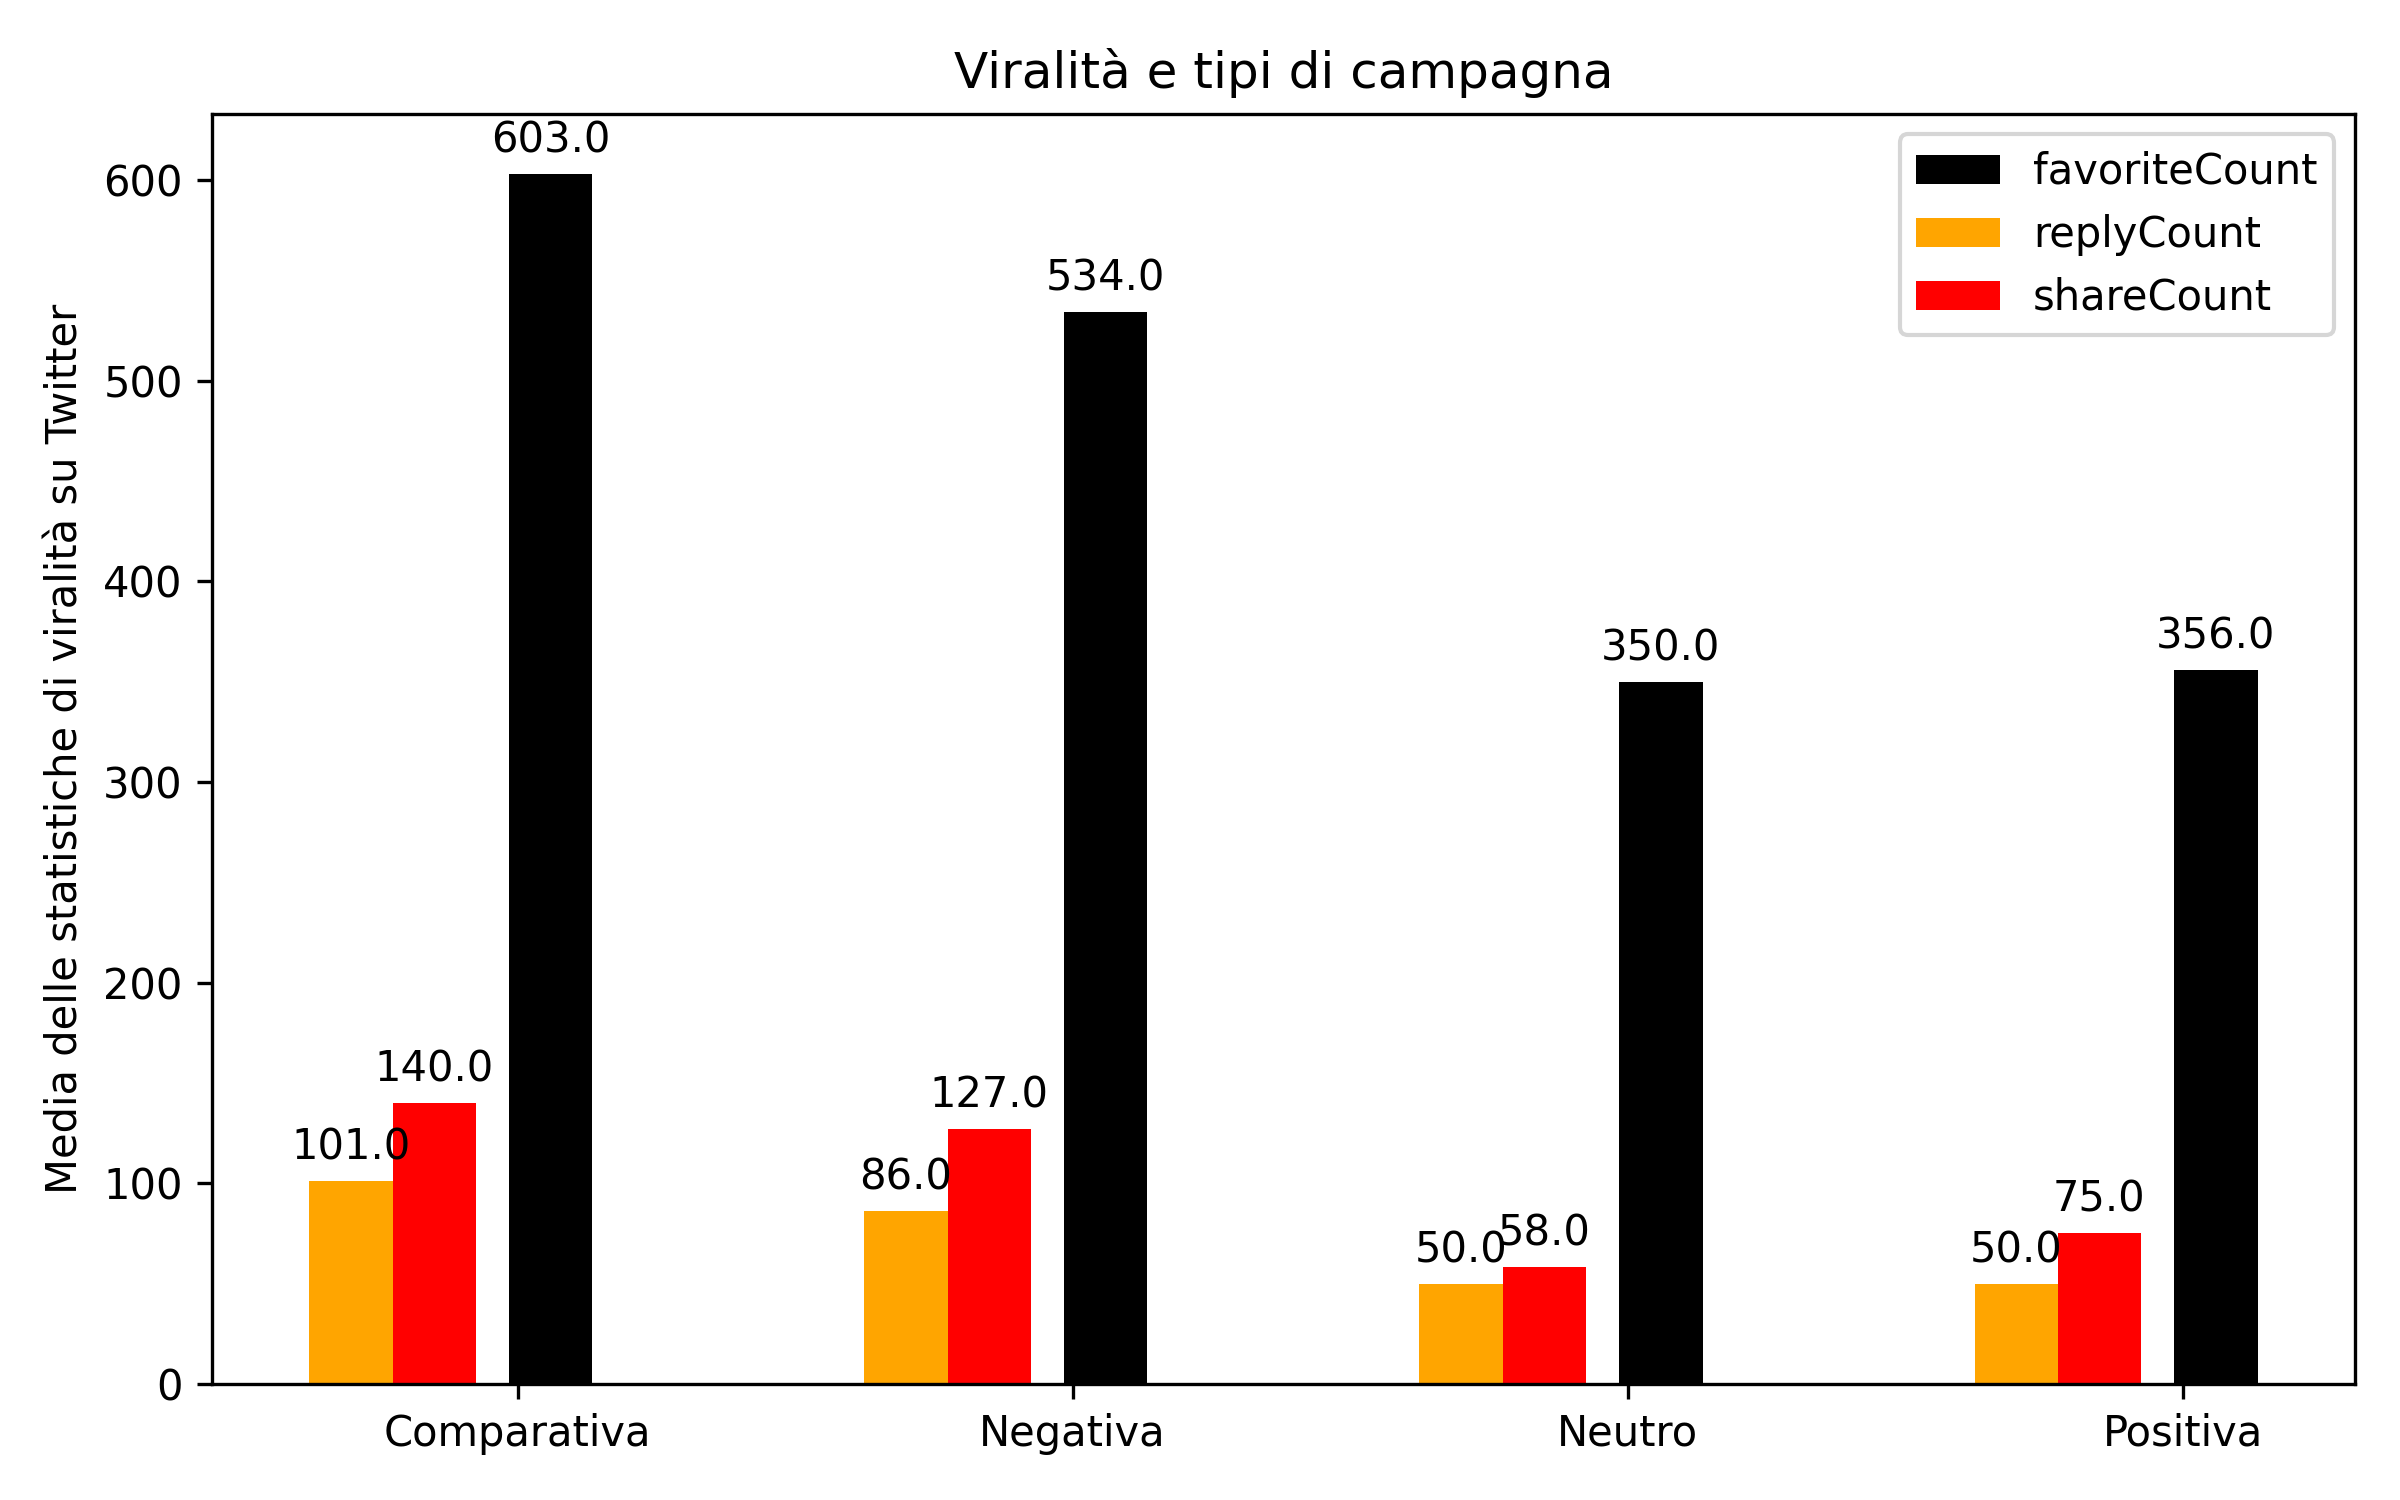
\includegraphics[width=\linewidth]{figures/viralitatw}
		\captionof{figure}{Differenza tra le medie dei principali indicatori di viralità e i tipi di campagna politica su Twitter.}
		\label{fig:viralitatw}
	\end{minipage}%
	\begin{minipage}{.5\textwidth}
		\centering
		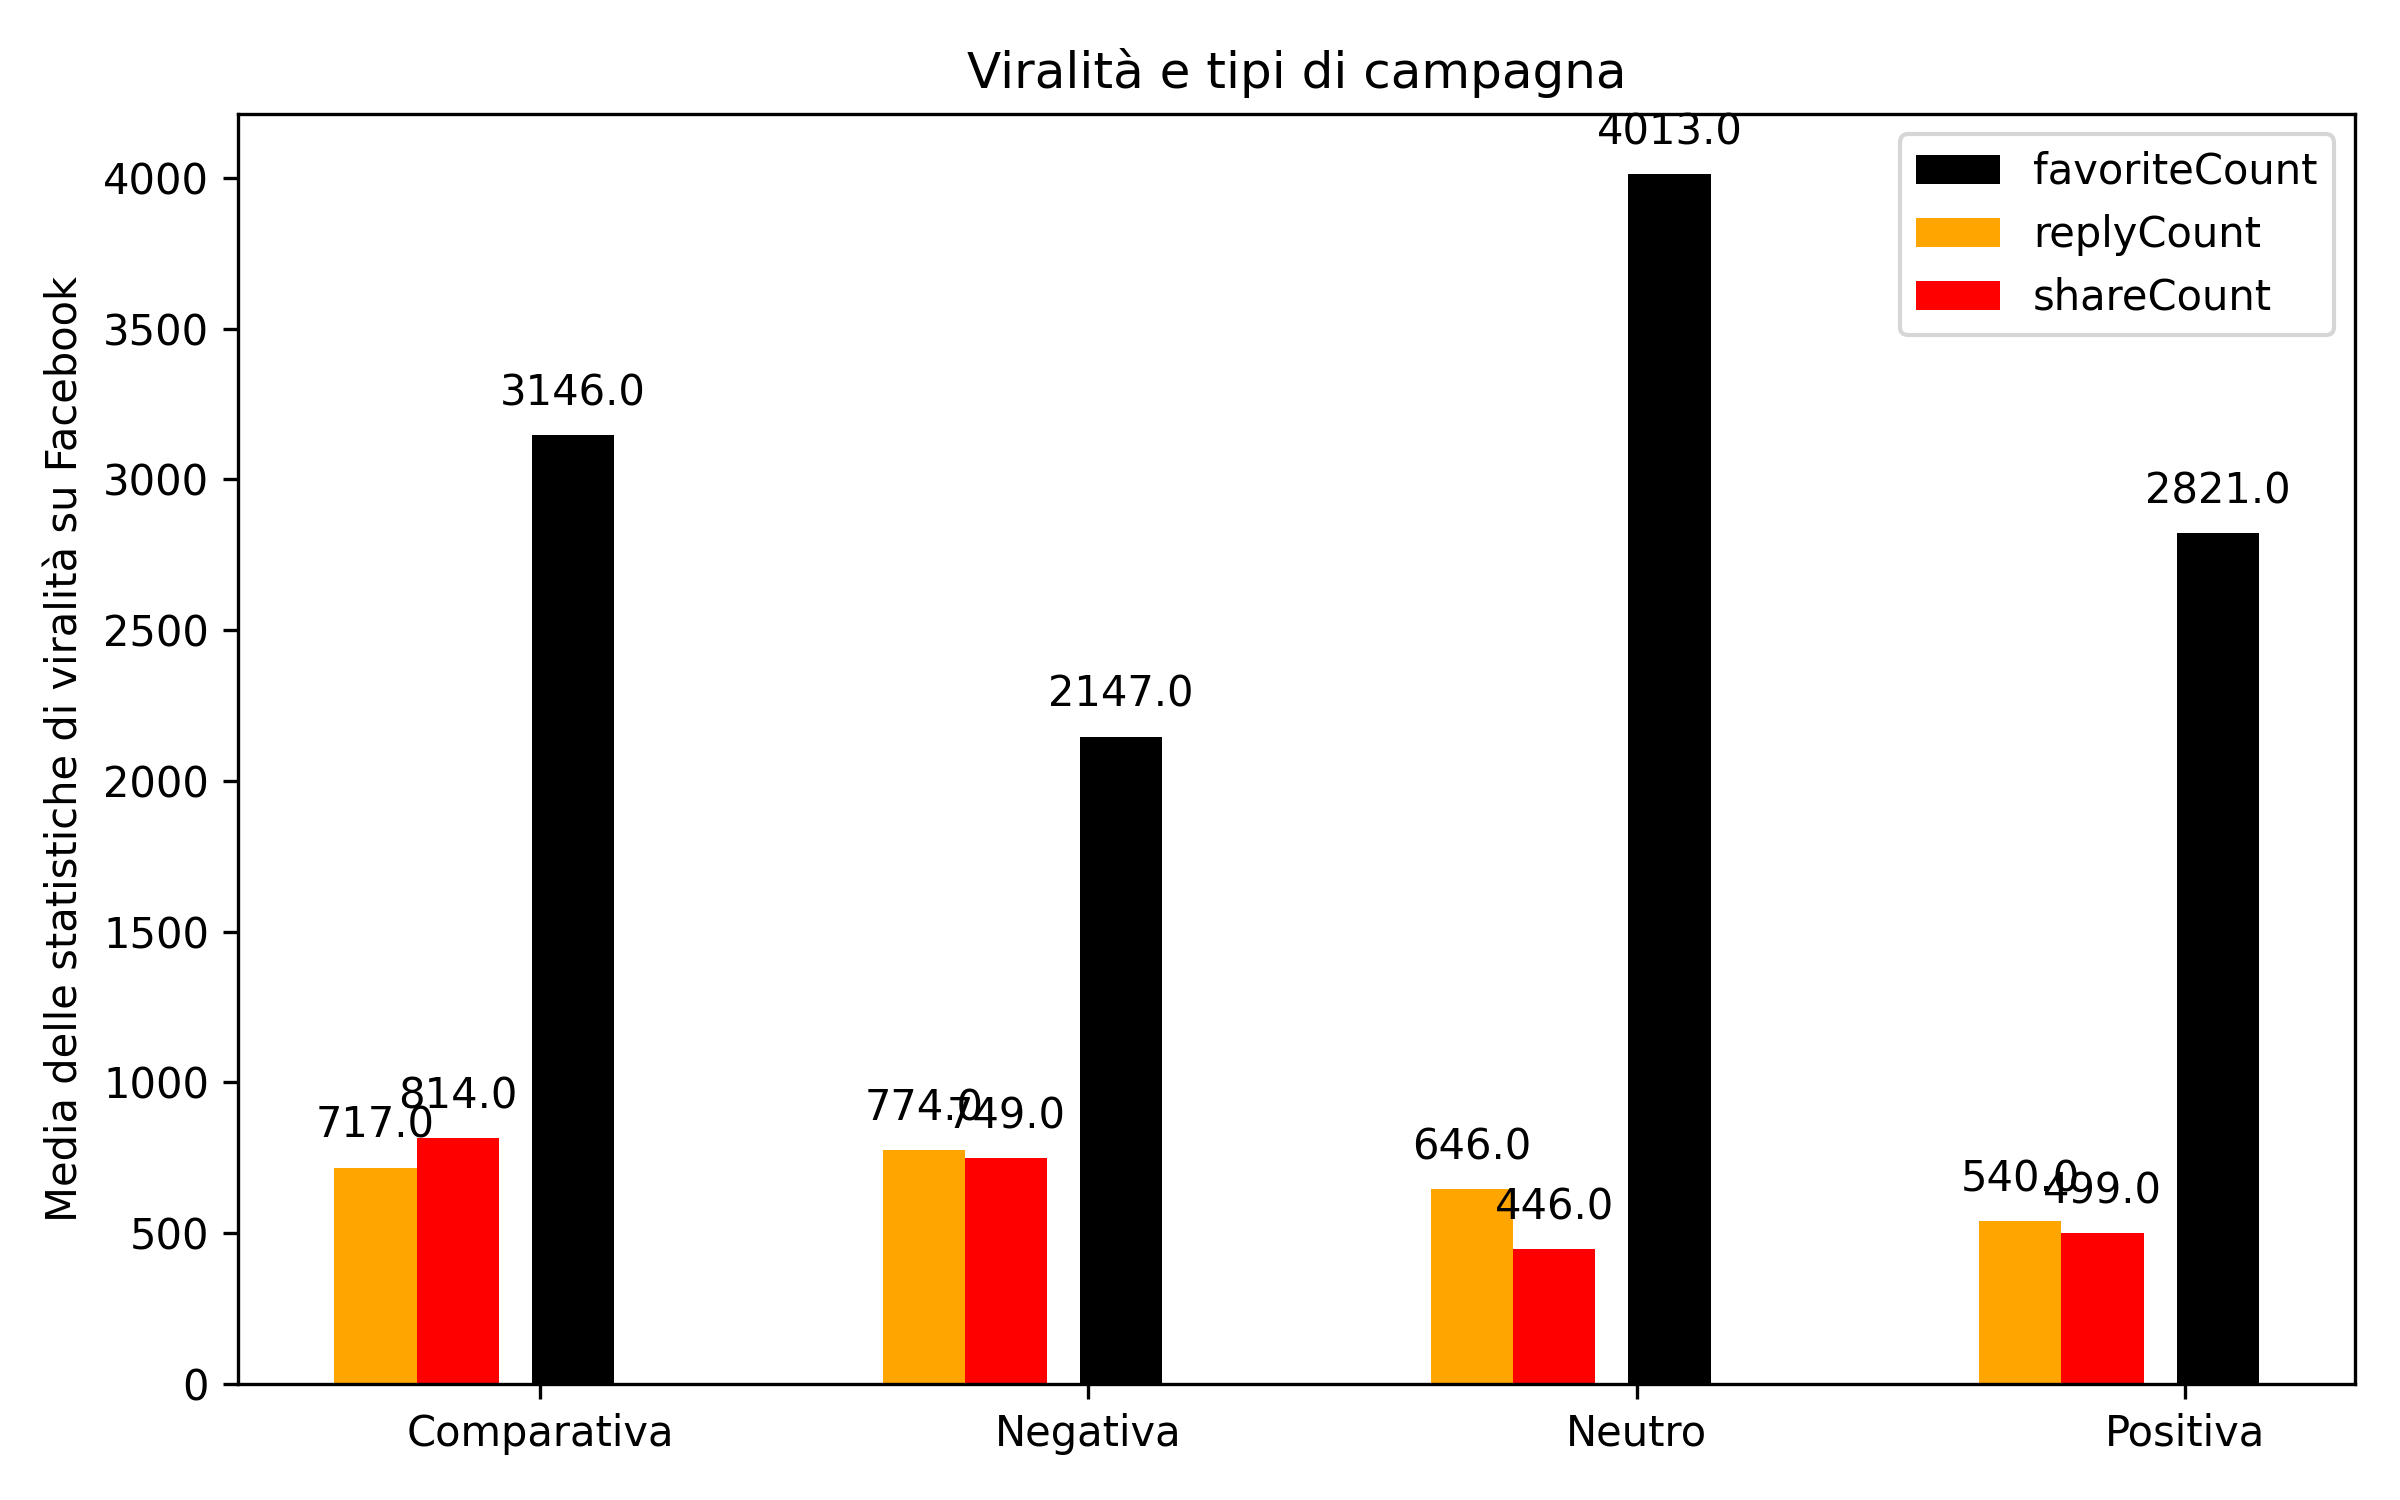
\includegraphics[width=\linewidth]{figures/viralitafb}
		\captionof{figure}{Differenza tra le medie dei principali indicatori di viralità e i tipi di campagna politica su Facebook.}
		\label{fig:viralitafb}
	\end{minipage}
\end{figure}
\begin{figure}
	\centering
	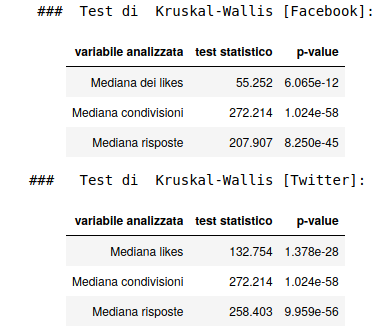
\includegraphics[width=0.65\textwidth]{figures/testmediane}
	\caption{Risultati del test di Kruskal-Wallis sulla viralità in base al tipo di campagna utilizzato. Tutte le differenze di mediana risultano largamente significative}
	\label{fig:testmediane}
\end{figure}
A parte la piccola anomalia della media di likes riscontrata nei post negativi su Facebook, che potrebbe in qualche modo spiegare il perché questo tipo di campagna venga utilizzata meno sul social di Zuckerberg rispetto a Twitter, come discusso nell'ipotesi 3, la letteratura e l'ipotesi iniziale qui presa in considerazione risultano confermate: la negatività dei messaggi politici è in grado di aumentare la diffusione dei contenuti.

Per testare la significatività delle differenze tra i gruppi presi in considerazione, è stato utilizzato il test di Kruskal-Wallis. La numerosità dei post che compongono tutte le categorie relative ai tipi di campagna utilizzata non è omogenea e gli assiomi dell'analisi della varianza non risultano verificati (la distribuzione dei valori non è normale, le rispettive varianze non risultano omogenee). Risulta quindi impossibile confrontare direttamente le medie con test come One-Way-ANOVA. Si ricorre quindi all'utilizzo delle mediane, che sono indici più robusti, e possono essere confrontate anche in casi come questo.
I risultati [Fig. \ref{fig:testmediane}] confermano quanto già osservato nei grafici precedenti: i sei test effettuati (per confrontare i tre indici di viralità per le due piattaforme) restituiscono in tutti i casi p-value significativi e valori della statistica di test in media sopra i 100 punti. L'ipotesi risulta quindi pienamente confermata anche da questo punto di vista.


\section{L'odio nei commenti}
In questa sezione cercheremo di indagare la relazione tra l'odio online registrato nei commenti e i post pubblicati dai politici. Verranno considerati quindi tutti i 78175 commenti categorizzati in base ai livelli di odio e i 10103 post analizzati in base al tipo di campagna politica.
\begin{wrapfigure}{r}{8cm}
	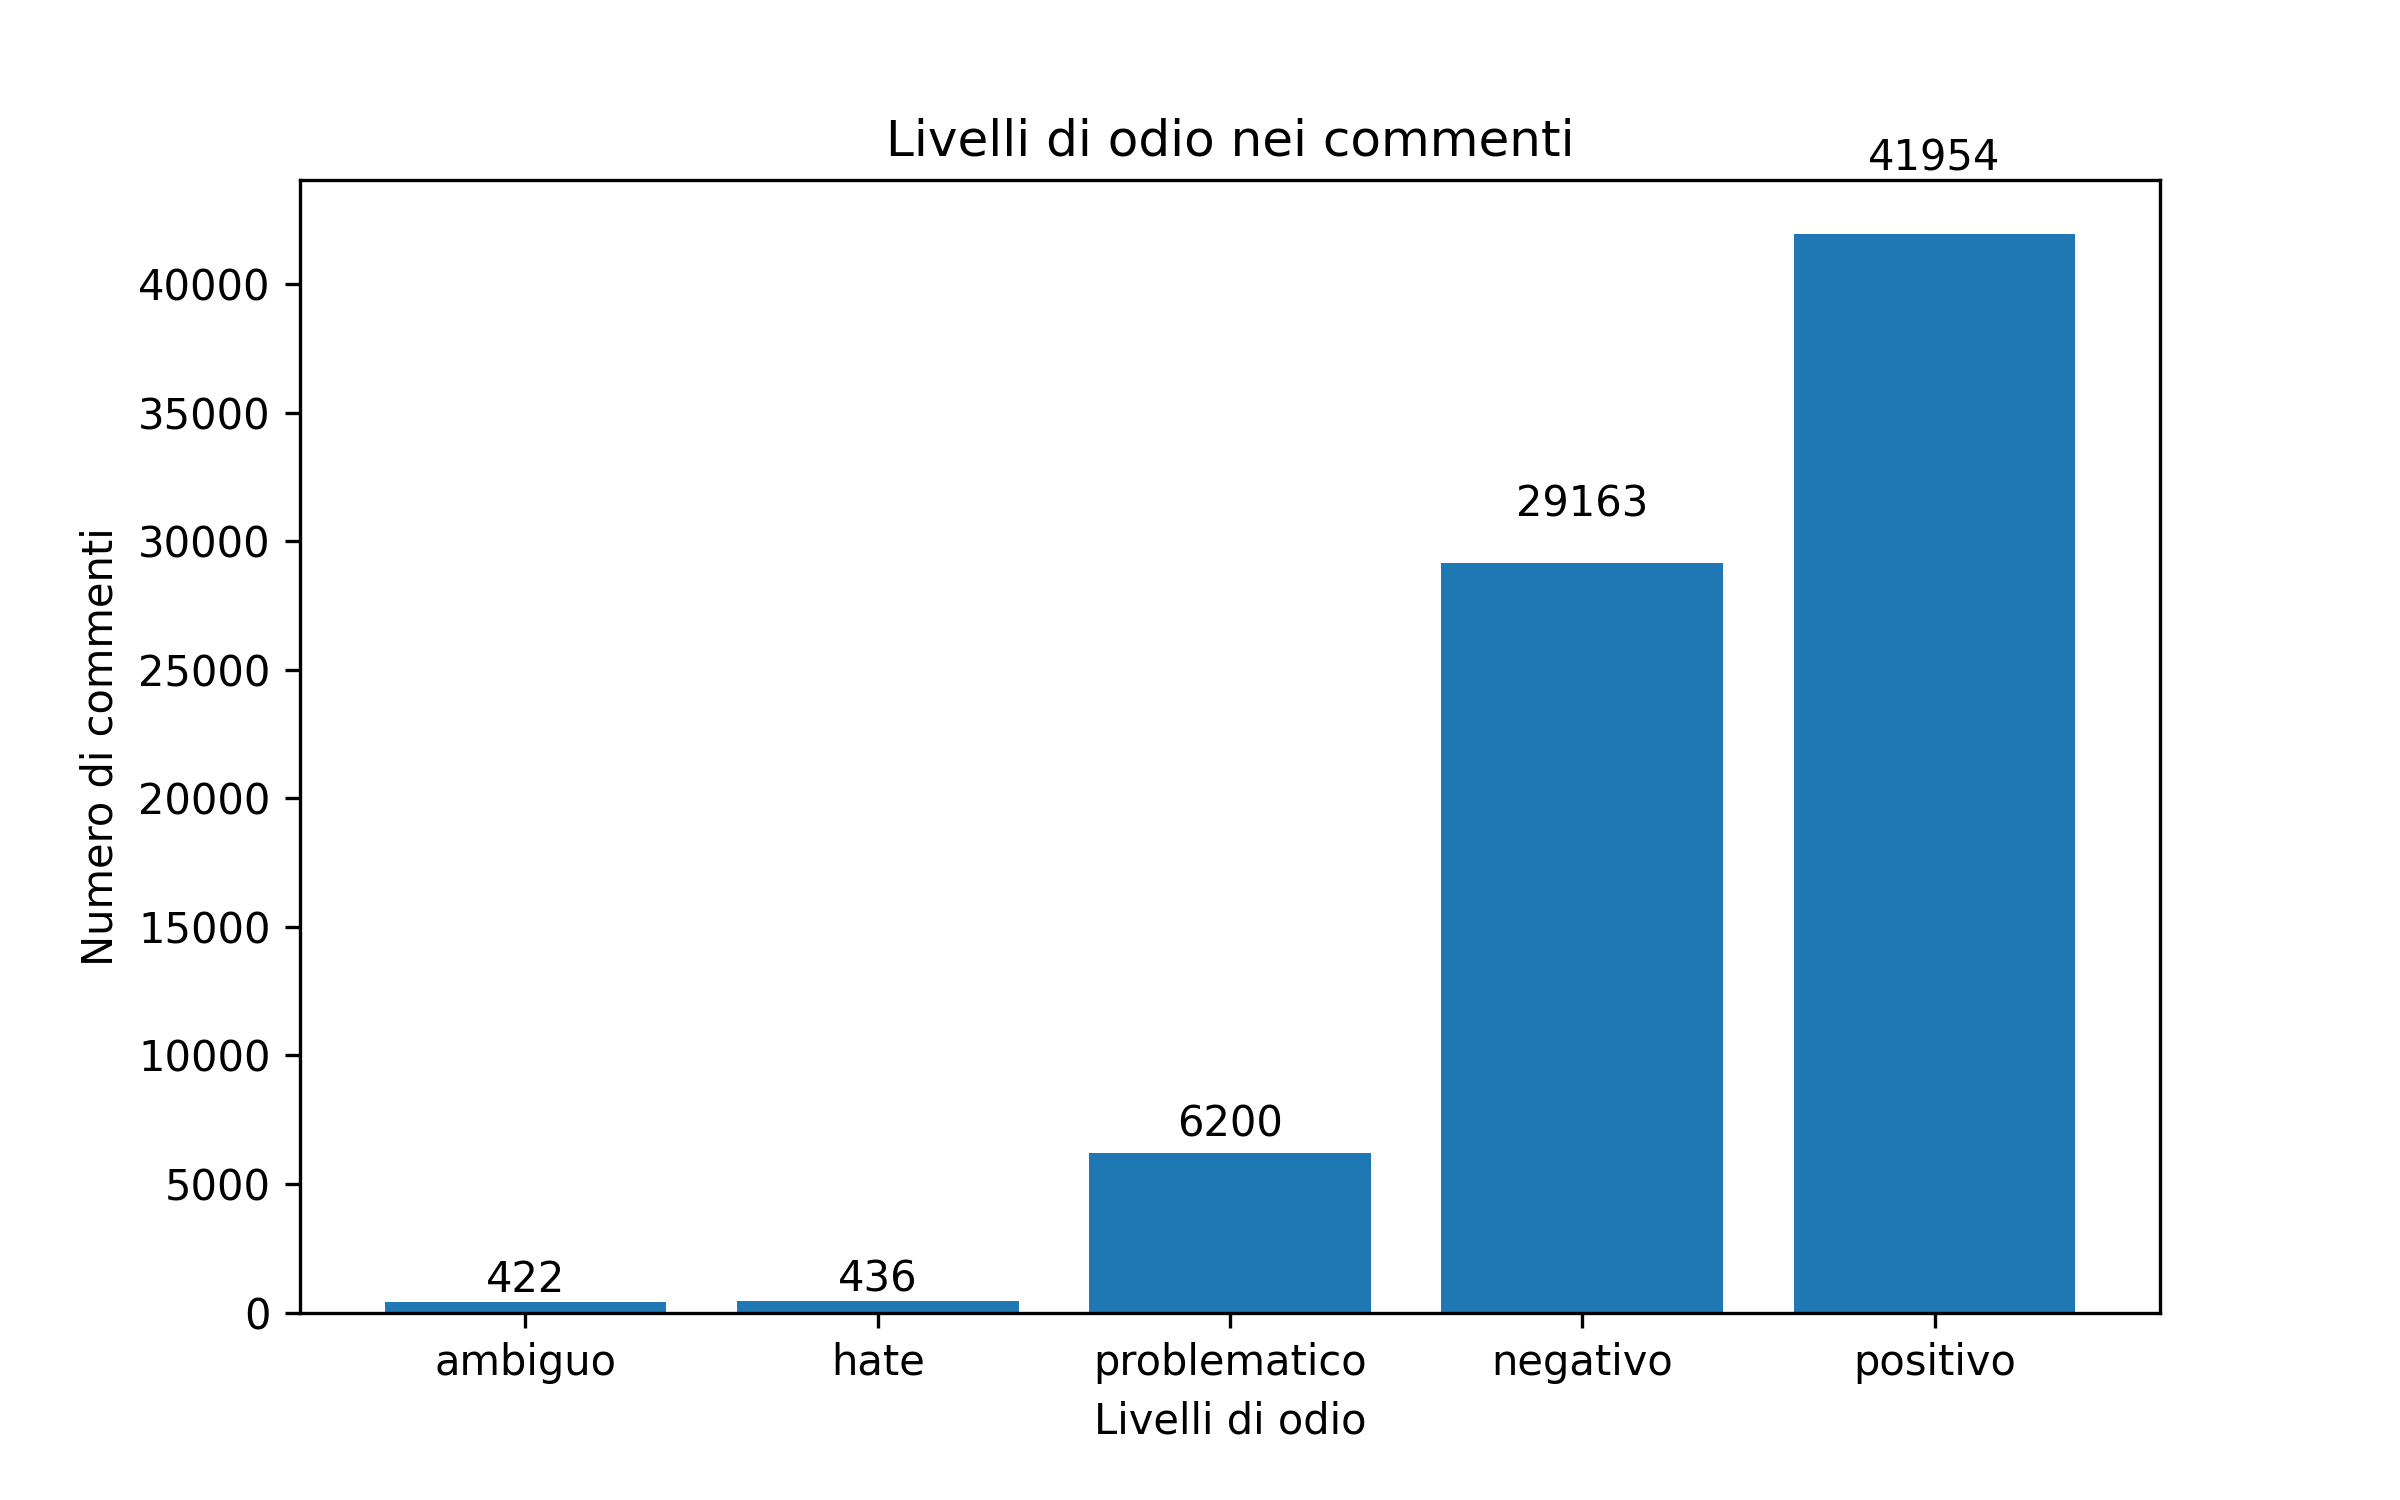
\includegraphics[width=8cm]{figures/odio}
	\caption{Livelli di odio generali riscontrati all'interno del campione}
	\label{odio3}
\end{wrapfigure}

Relativamente alla dimensione generale del fenomeno, va segnalato che i livelli generali di odio registrati già nello studio di Amnesty (vedi capitolo "\nameref{chap:metodologia}"), evidenziano un problema che forse, in questo caso, potrebbe risultare minore delle aspettative dell’opinione pubblica. Se tra i post dei politici solo un contenuto è stato classificato come propriamente \textit{hate speech}, tra i commenti ne sono stati codificati 436 (1\%) [Fig.~\ref{odio3}].

Percentuali più rilevanti sono riscontrate per i messaggi degli utenti che utilizzano linguaggio incivile pur senza sfociare nella discriminazione di minoranze a rischio: 6200 casi equivalenti all'8\% del campione. Sicuramente il tipo di contenuti prevalenti è quello positivo 54\%, seguito dai commenti negativi, ma civili, che valgono il 34\% del totale.

È importante sottolineare che prendendo in considerazione i commenti relativi ai post, le percentuali in cui i vari tipi di campagna sono presenti è differente rispetto al campione costituito dai i soli post [Fig.~\ref{tipoDiCampagnapie2}]. Il numero di commenti raccolti e poi analizzati per ogni post di politico dipende dalla numerosità dei commenti presenti in relazione a quello specifico contenuto, ed è stata pensata per comporre un campione rappresentativo di tutti i politici in corsa alle elezioni e del loro effettivo seguito sui social.

\begin{wrapfigure}{l}{8cm}
	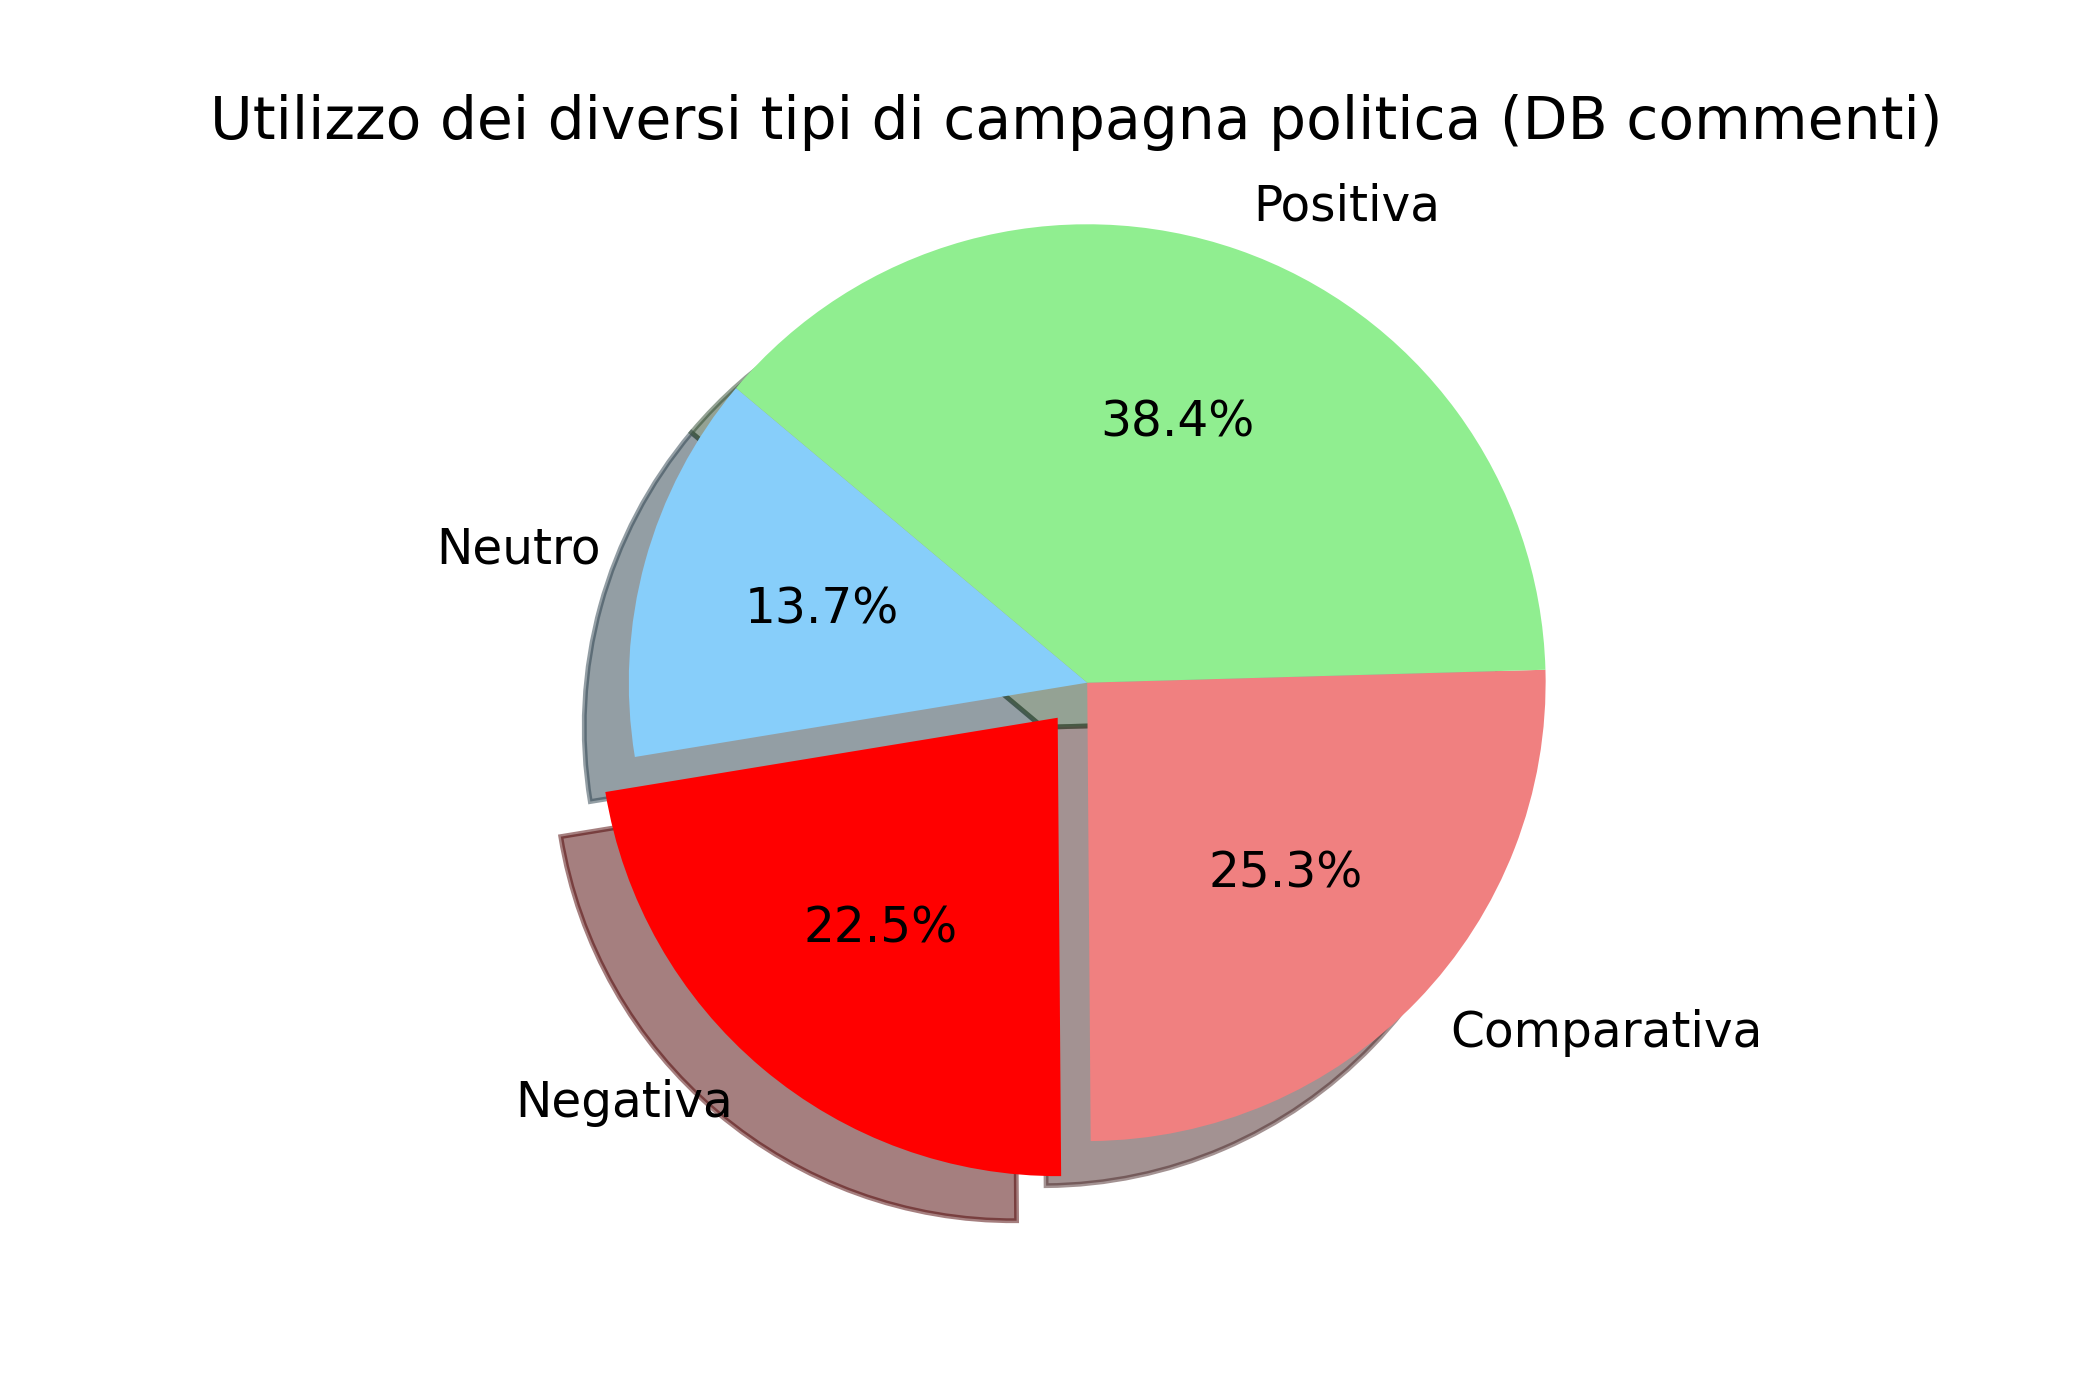
\includegraphics[width=8cm]{figures/tipoDiCampagnapie2}
	\caption{Percentuali dei tipi di campagna riscontrati nel database dei commenti}
	\label{tipoDiCampagnapie2}
\end{wrapfigure}

Il campione non è stato pensato per essere omogeneo nei tipi di campagna politica, che comunque sono stati categorizzati in un momento successivo allo studio de "Il barometro dell'odio". La differenza nella variazione delle percentuali non è in nessun modo spiegabile o legata a questo studio, dipende piuttosto dal campionamento e ha come effetto delle variazioni non tali da invalidare le successive analisi, ma comunque degne di essere spiegate. Per chiarire con un esempio: il numero di commenti di risposta ai post negativi non hanno la stessa percentuale sul totale dei commenti (22,5\%) che hanno i post negativi sul totale dei post (16\%). Lo stesso vale per i commenti di post comparativi (25\% rispetto al 19,2\% nel campione dei soli post) e per quelli positivi (38,4\% rispetto al 52\%). Le categorie negative e comparative risultano quindi sovradimensionate, come abbiamo avuto modo di spiegare nelle precedenti ipotesi, questi tipi di campagna risultano più virali e quindi anche più commentate. Ciò ci porta ad avere più commenti per post nel campione complessivo che è proporzionato al numero di risposte ad ogni contenuto di politico. Questo non dovrebbe però influire sul tipo di analisi che faremo nei prossimi sottoparagrafi, che partono dall'assunto che i tipi di campagna non sono comunque rappresentati in egual misura e vengono quindi comparati in base alle percentuali di commenti negativi tramite test di chi-quadro.

\subsection{Ip.1: Il \textit{negative campaign}  genera più odio nei commenti?}
Questa domanda risulta essere quella  principale all'interno di questo studio poiché permette di sfruttare al meglio tutte le potenzialità del database, utilizzando contemporaneamente post e relativi commenti.

Dai valori assoluti dei contenuti di odio presenti nei commenti  [Fig. \ref{fig:hate}] possiamo già fare delle considerazioni. L'\textit{hate speech} compare in uguale misura nelle reazioni a post comparativi e negativi, con valori molto più alti rispetto ai post positivi, nonostante i commenti relativi a questo tipo di post siano più numerosi. I commenti positivi mostrano, invece, un andamento diametralmente opposto. I commenti problematici fanno registrare il valore assoluto più alto in risposta a post comparativi, e risultano uguali in risposta a campagne negative e positive, nonostante la disparità di numero di commenti totale. Interessante che la campagna comparativa faccia registrare più commenti positivi che negativi, mentre nei post negativi avviene il contrario.
\begin{figure}
	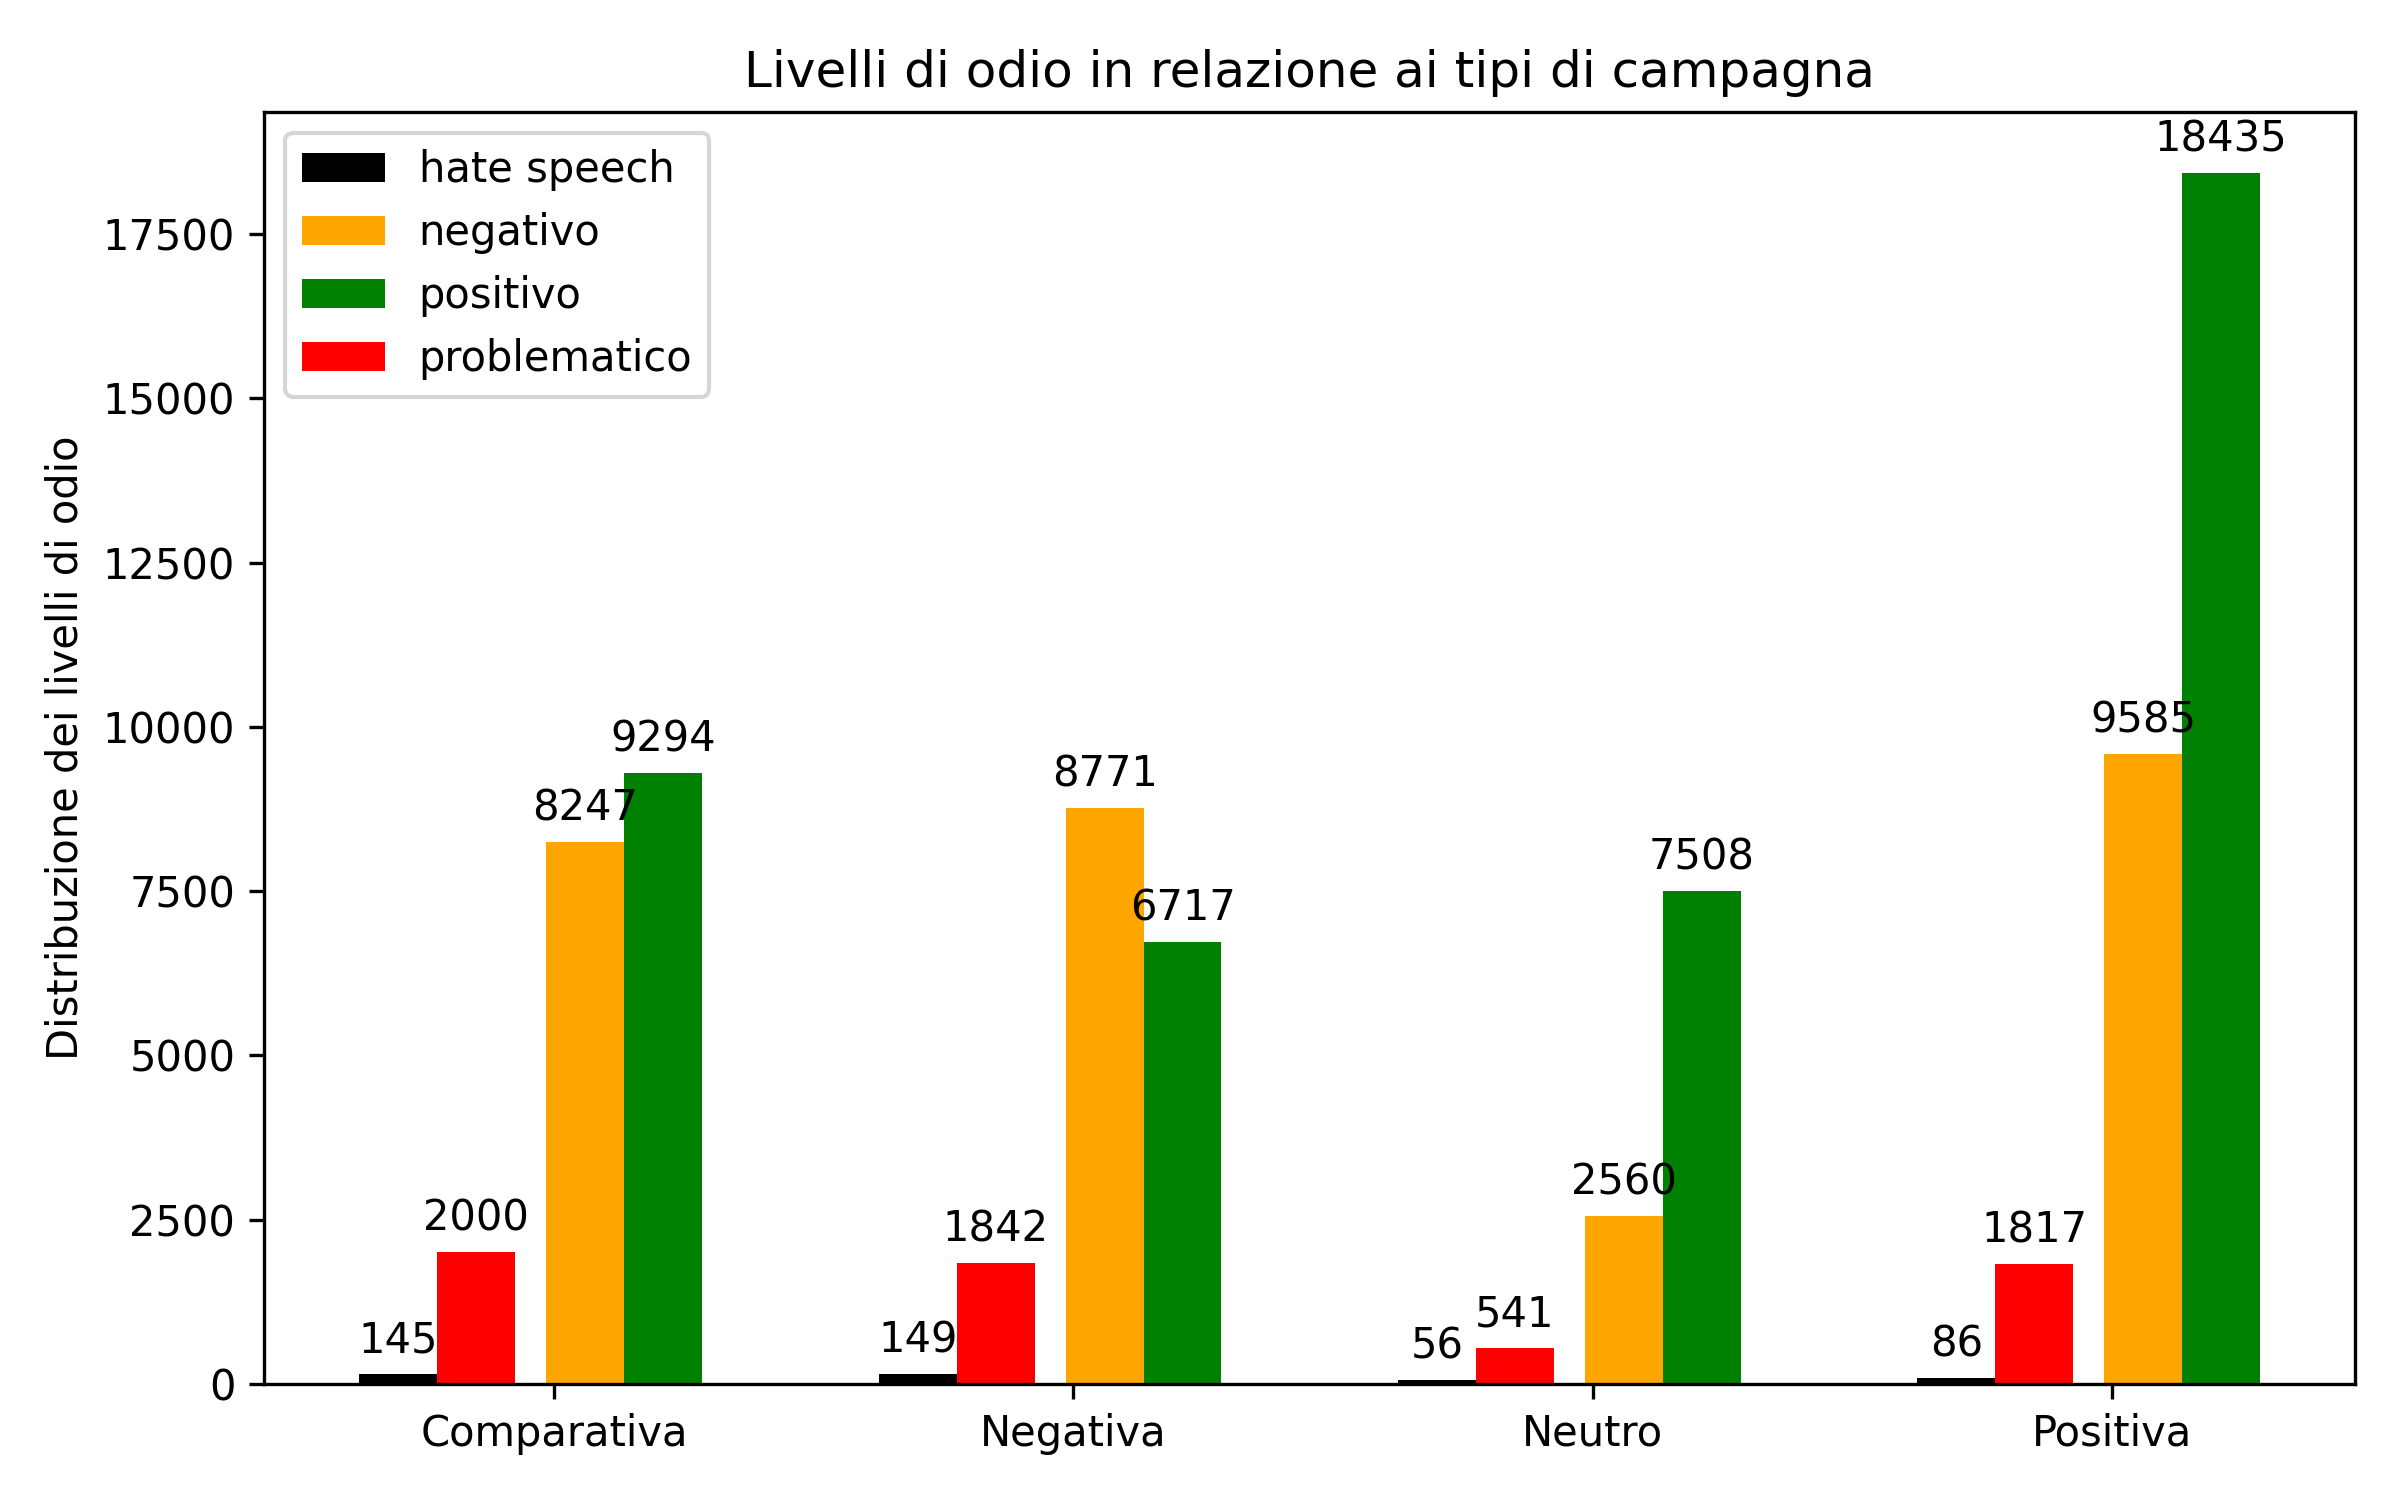
\includegraphics[width=\textwidth]{figures/hate}
	\caption{Valori assoluti dei livelli di odio in relazione con i tipi di campagna politica.}
	\label{fig:hate}
\end{figure}

Per contestualizzare meglio i valori assoluti, è utile vedere come il numero dei vari tipi di commenti si rapporta con il totale dei commenti di ogni tipo di campagna. Per farlo sono state calcolate le percentuali delle categorie dei commenti in base alle categorie dei post dei politici [Fig. \ref{fig:hatepercent1}]. Da qui emerge ancora più chiaramente come i commenti problematici siano più prevalenti quando il politico cita l'avversario nei suoi post: in risposta alla campagna negativa si supera il 10\%, poco sotto si collocano i commenti a post comparativi, mentre la percentuale di questo tipo di risposta per i positivi si ferma a quasi la metà . In generale da questo tipo di grafico si comprende meglio come i post negativi generano le maggiori percentuali di tutti i tipi di contenuti classificabili come \textit{hate speech}, problematici, e negativi.
\begin{figure}
	\centering
	\begin{minipage}{.5\textwidth}
		\centering
		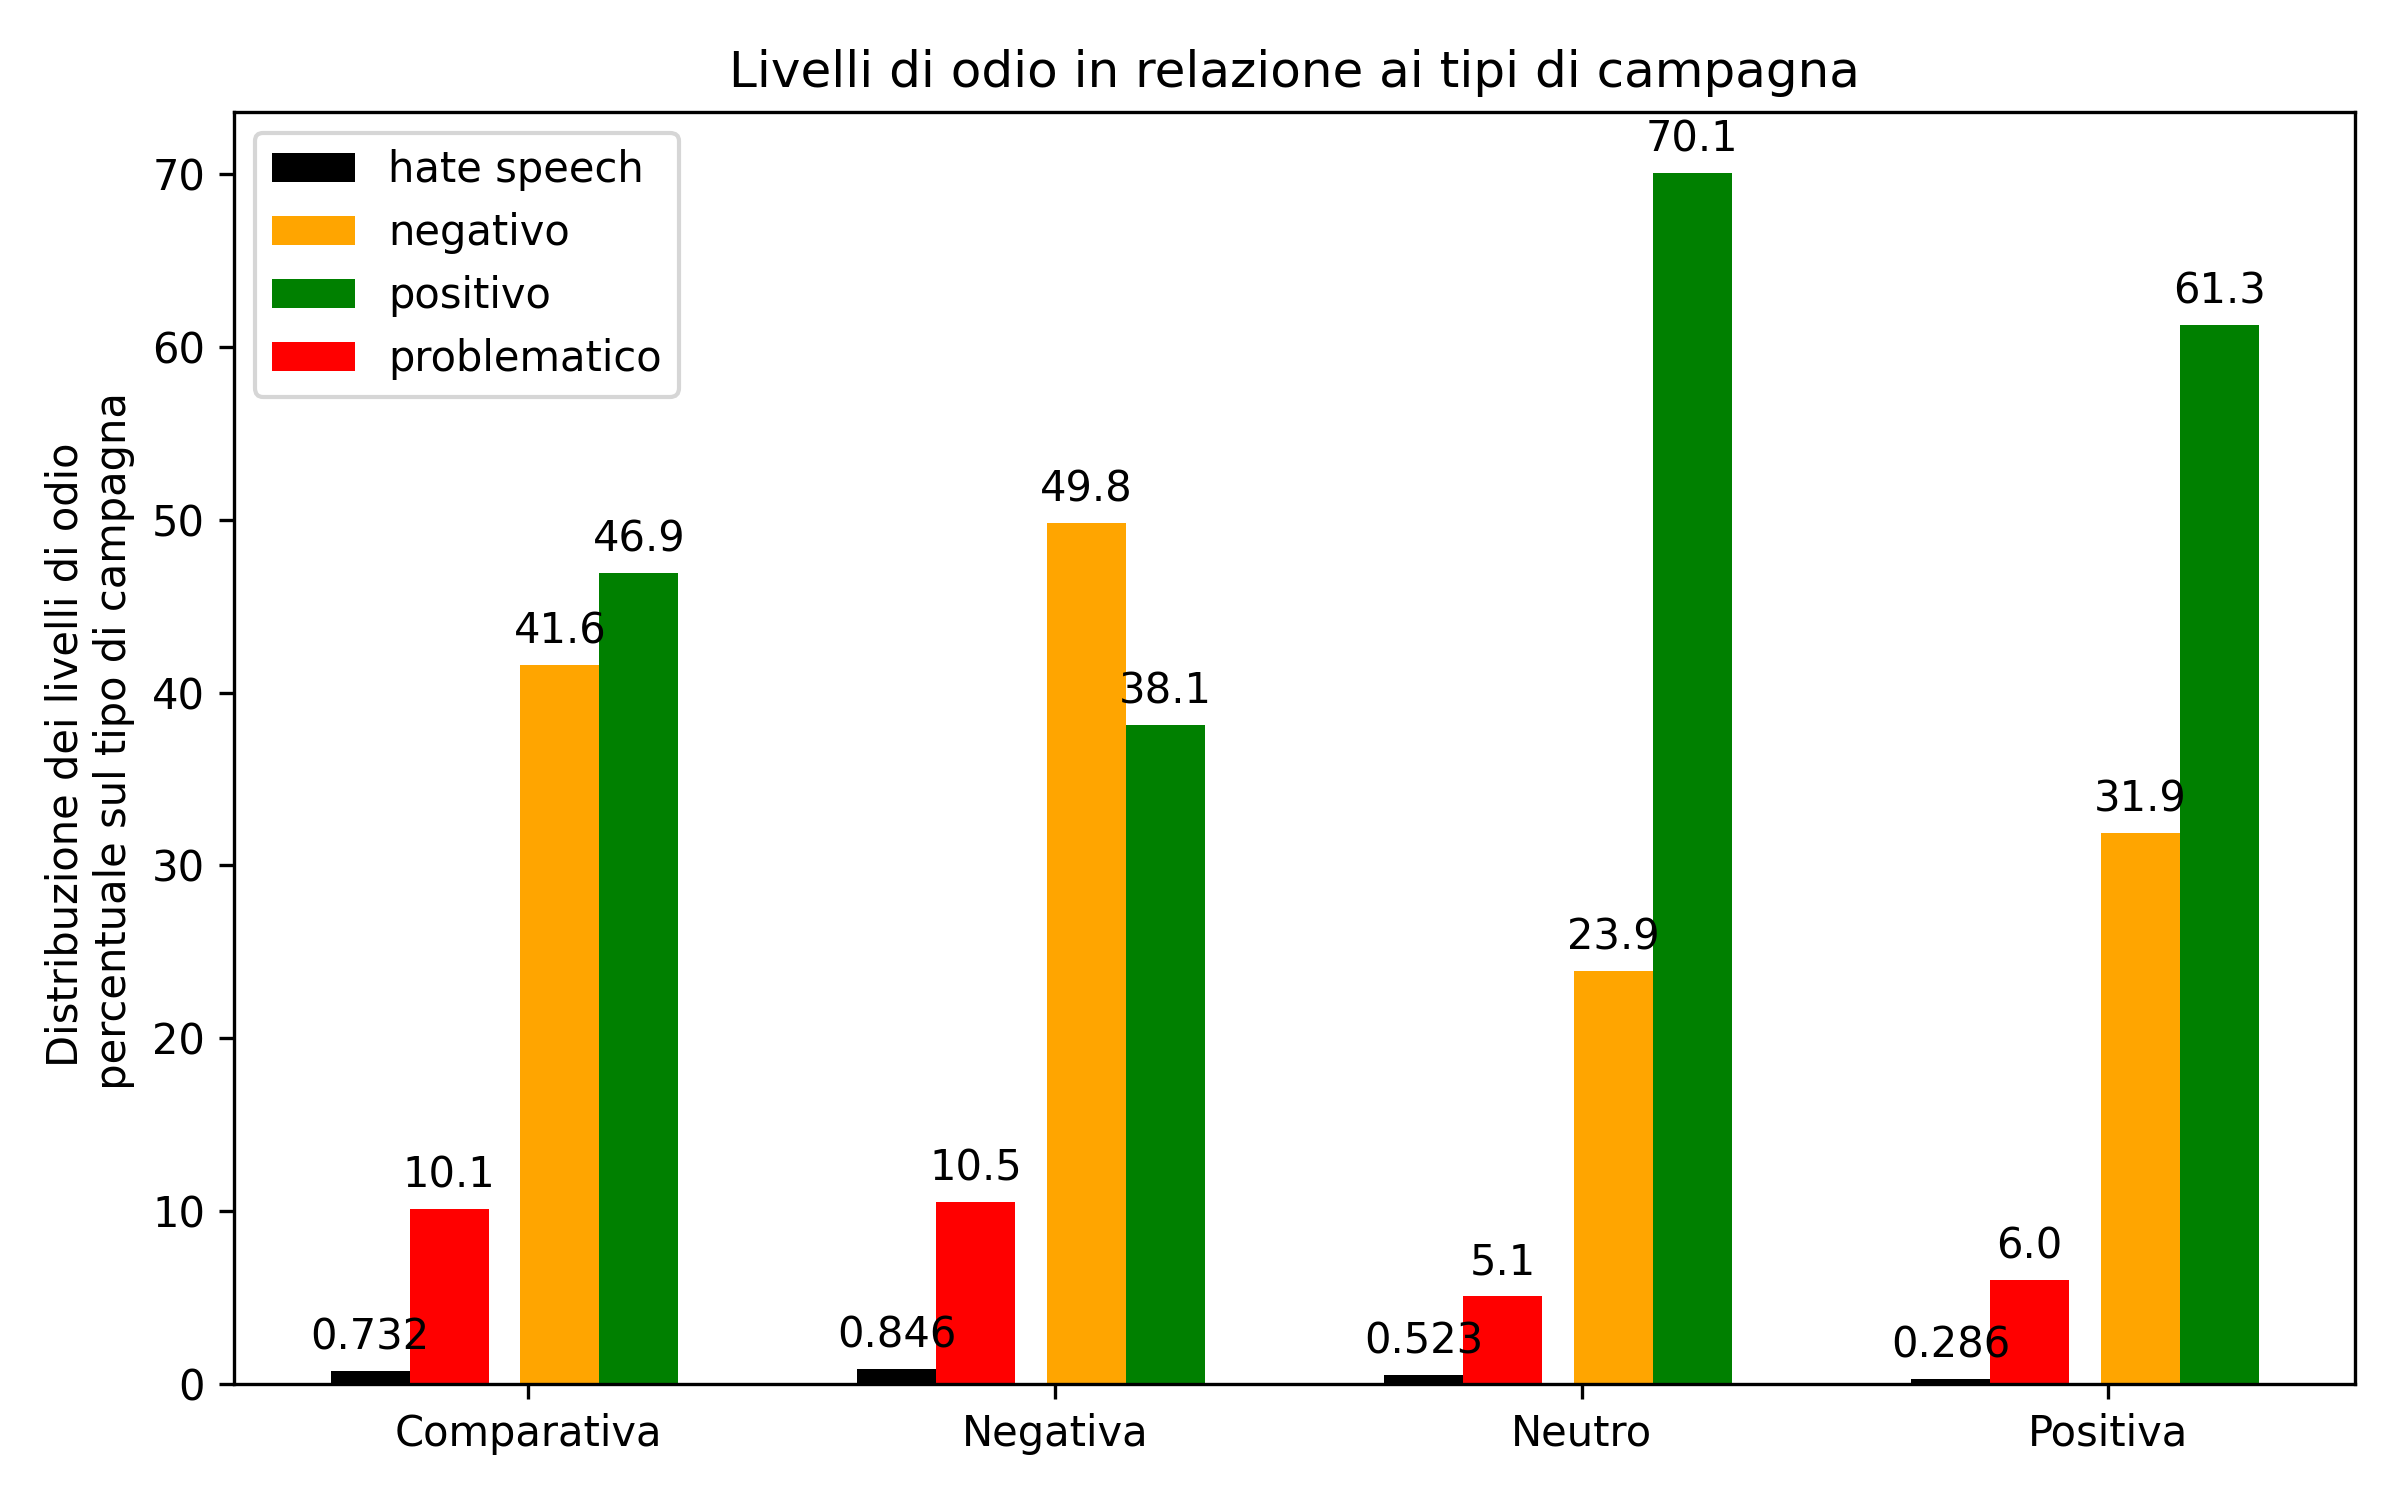
\includegraphics[width=\linewidth]{figures/hatepercent1}
		\captionof{figure}{Livelli di odio nei commenti in relazione ai tipi di campanga politica. Percentuali relative al totale di tipo di campagna}
		\label{fig:hatepercent1}
	\end{minipage}%
	\begin{minipage}{.5\textwidth}
		\centering
		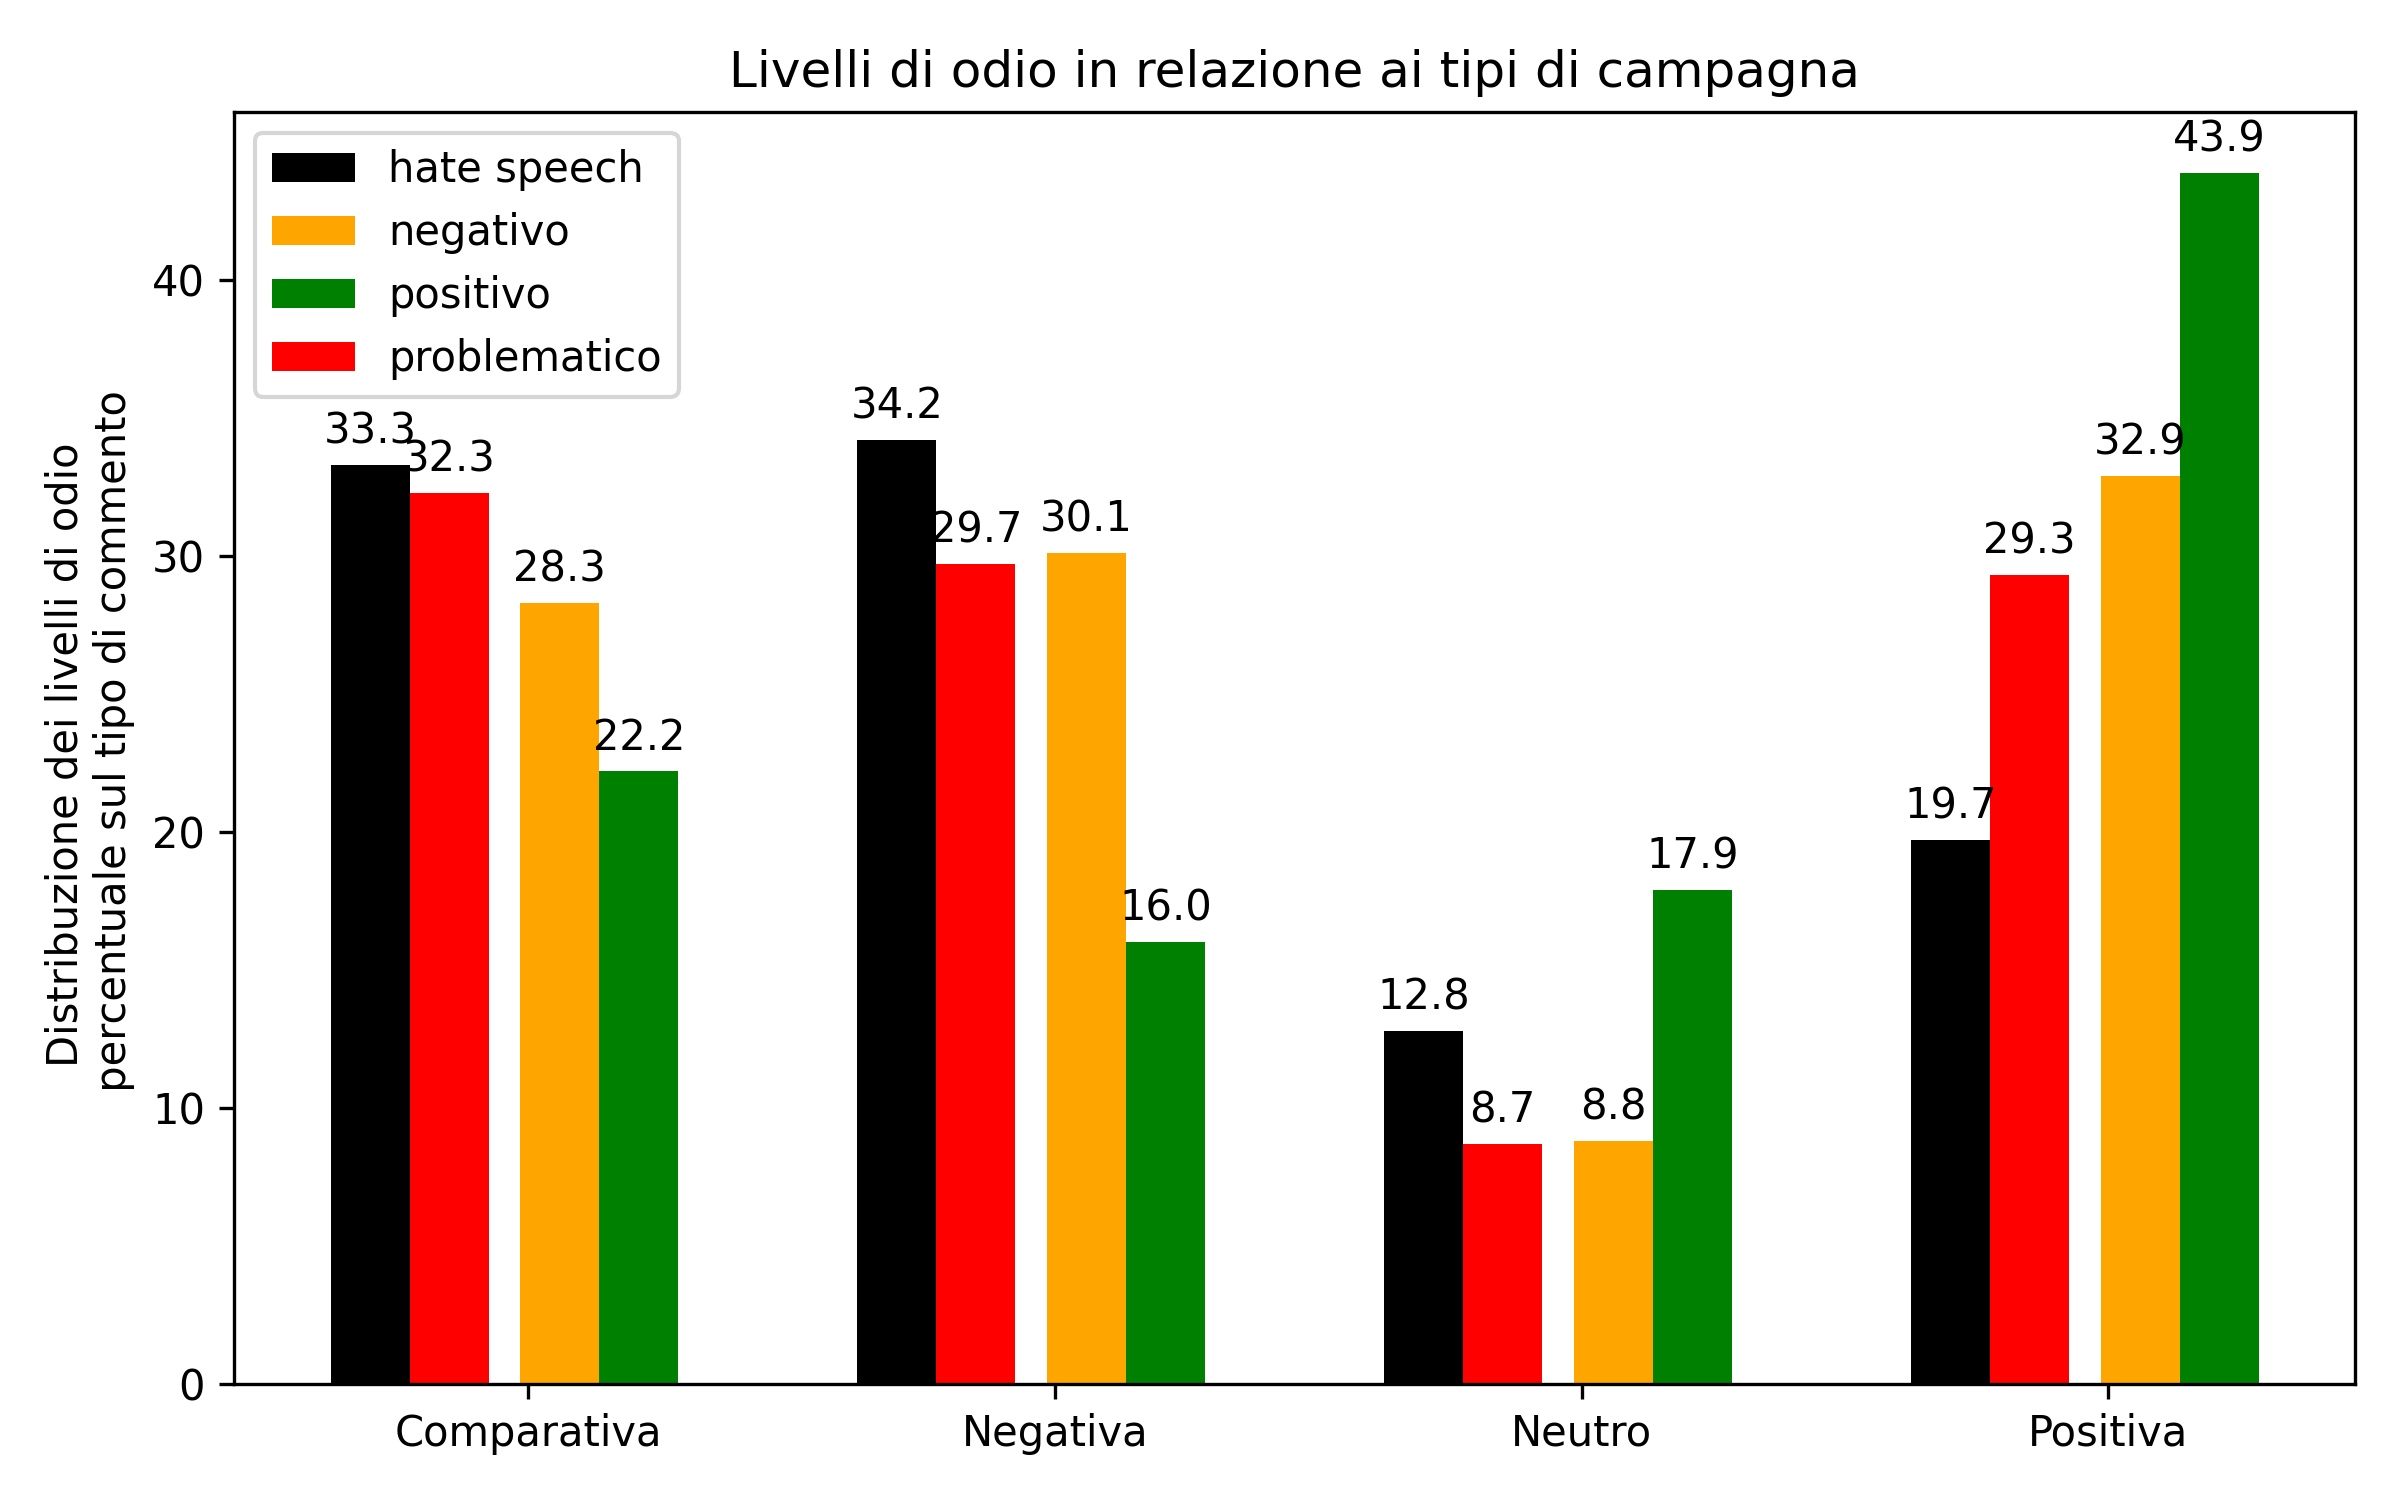
\includegraphics[width=\linewidth]{figures/hatepercent}
		\captionof{figure}{Livelli di odio nei commenti in relazione ai tipi di campanga politica. Percentuali relative al totale alle categorie dei livelli di odio}
		\label{fig:hatepercent}
	\end{minipage}
\end{figure}
Effettuando un test di chi-quadro, le differenze nelle frequenze risultano significative con un valore del test di Person molto alto e un p-value molto basso, avvalorando ulteriormente la conferma delle ipotesi: $\chi^{2}$ (7, N = 78175) = 4024.679, p = 0.0000.
%[Fig. \ref{fig:chihate}]
%\begin{figure}
%    \centering
%    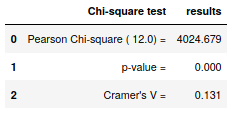
\includegraphics[width=0.5\textwidth]{figures/chihate}
%    \caption{Risultati del test di chi-quadro sui diversi livelli di odio in base ai tipi di campagna politica. Le differenze risultano significative.}
%    \label{fig:chihate}
%\end{figure}

Il ruolo cruciale del \textit{negative campaig}n nel generare odio emerge in modo ancora più evidente se si fa riferimento alla ripartizione dell' \textit{hate speech} per tipologia dei post che lo ha generato. [Fig. \ref{fig:hatepercent}]. Risulta infatti che il 67,5\% di tutti i commenti di \textit{hate speech} sono stati registrati sotto i post che citano avversari. Senza questo tipo di campagna l'odio sarebbe poco più del  30\% del totale.
Da questo dato si possono trarre, quindi, indicazioni importanti per identificare delle strategie concrete utili per ridurre i livelli di odio presenti sul web. Evitare o ridurre campagne negative e comparative potrebbe ridurre conseguentemente anche i livelli di odio nei commenti. Indicazioni ancora più precise emergono dall’analisi del tipo di target indicato nelle campagne negative e comparativa.

\subsection{Ip.2: quale target genera più odio nei commenti?}
Prendendo in considerazione solo i post di campagna negativa e comparativa, possiamo analizzare i target che vengono maggiormente utilizzati in questo tipo di attacchi verbali e le conseguenze sui livelli di odio nei commenti. I post/tweet negativi e comparativi sono 3009, cioè il 30\% dei post prodotti. I commenti campionati in risposta a questi post sono 37413, il 44.8\% di tutti i commenti considerati. A partire da questo nuovo \textit{subset} potremo capire meglio cosa scatena la generazione di odio online.

Come si può vedere nel grafico [Fig.\ref{fig:target}], questo tipo di post può avere uno o due target contemporaneamente. Succede spesso, ad esempio, che ci si rivolga a un partito rivale, citando anche un avversario politico specifico, oppure che si metta in relazione un personaggio pubblico a uno schieramento e ai suoi temi. I post/tweet con doppio target sono 565, i commenti che fanno seguito a questi post con doppio target sono 6430. I commenti relativi a post con singolo target risultano quindi nettamente più frequenti: “personaggio politico” e “gruppo politico” insieme valgono il 56\% di tutti i commenti relativi a post negativi o comparativi (rispettivamente 23\% e 42\%) e valgono il 7\% quando compaiono insieme raggiungendo il 63\% totale, ben al di sopra di tutti gli altri tipi di target. I commenti relativi a post di attacco a “categorie di persone” rappresentano l'8\% del totale dei commenti di questo \textit{subset}, le risposte ad altri target singoli sono presenti in percentuali comprese tra il 2 e 4\%. Tutti i target doppi hanno generato meno dell'1\% dei commenti qui presi in considerazione.
\begin{figure}
	\centering
	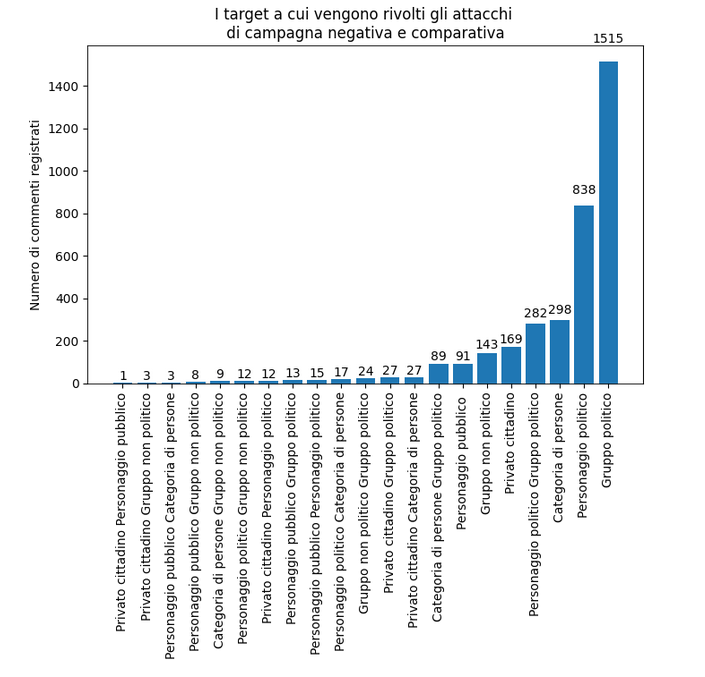
\includegraphics[width=0.85\textwidth]{figures/target}
	\caption{Percentuali dei tipi di campagna riscontrati nel database dei commenti}
	\label{fig:target}
\end{figure}

Per ridurre il numero di singole categorie prese in considerazione e per poter vedere più chiaramente la loro relazione con il tipo di commenti generato, ogni commento con target doppio è stato sdoppiato nei due target singoli. Questo metodo introduce una distorsione, aumentando il numero di singoli commenti presi in considerazione da 37413 a 43648 elementi, considerando che 6430 vengono sostanzialmente sdoppiati, ma la distorsione non è tale da inficiare le indicazioni qualitative delle nostre elaborazioni. Inoltre, sempre per questioni di semplicità, nei grafici, non verranno presentati i risultati relativi ai commenti codificati come ambigui, dato che per queste risposte non è stato possibile, in fase di codifica, capire il significato, risultano meno importanti per le considerazioni che andremo a fare. Queste semplificazioni non verranno, però, conservate  nel corso delle analisi statistiche necessarie a confermare la significatività dei risultati finali relativi a questa ipotesi.
\begin{figure}
	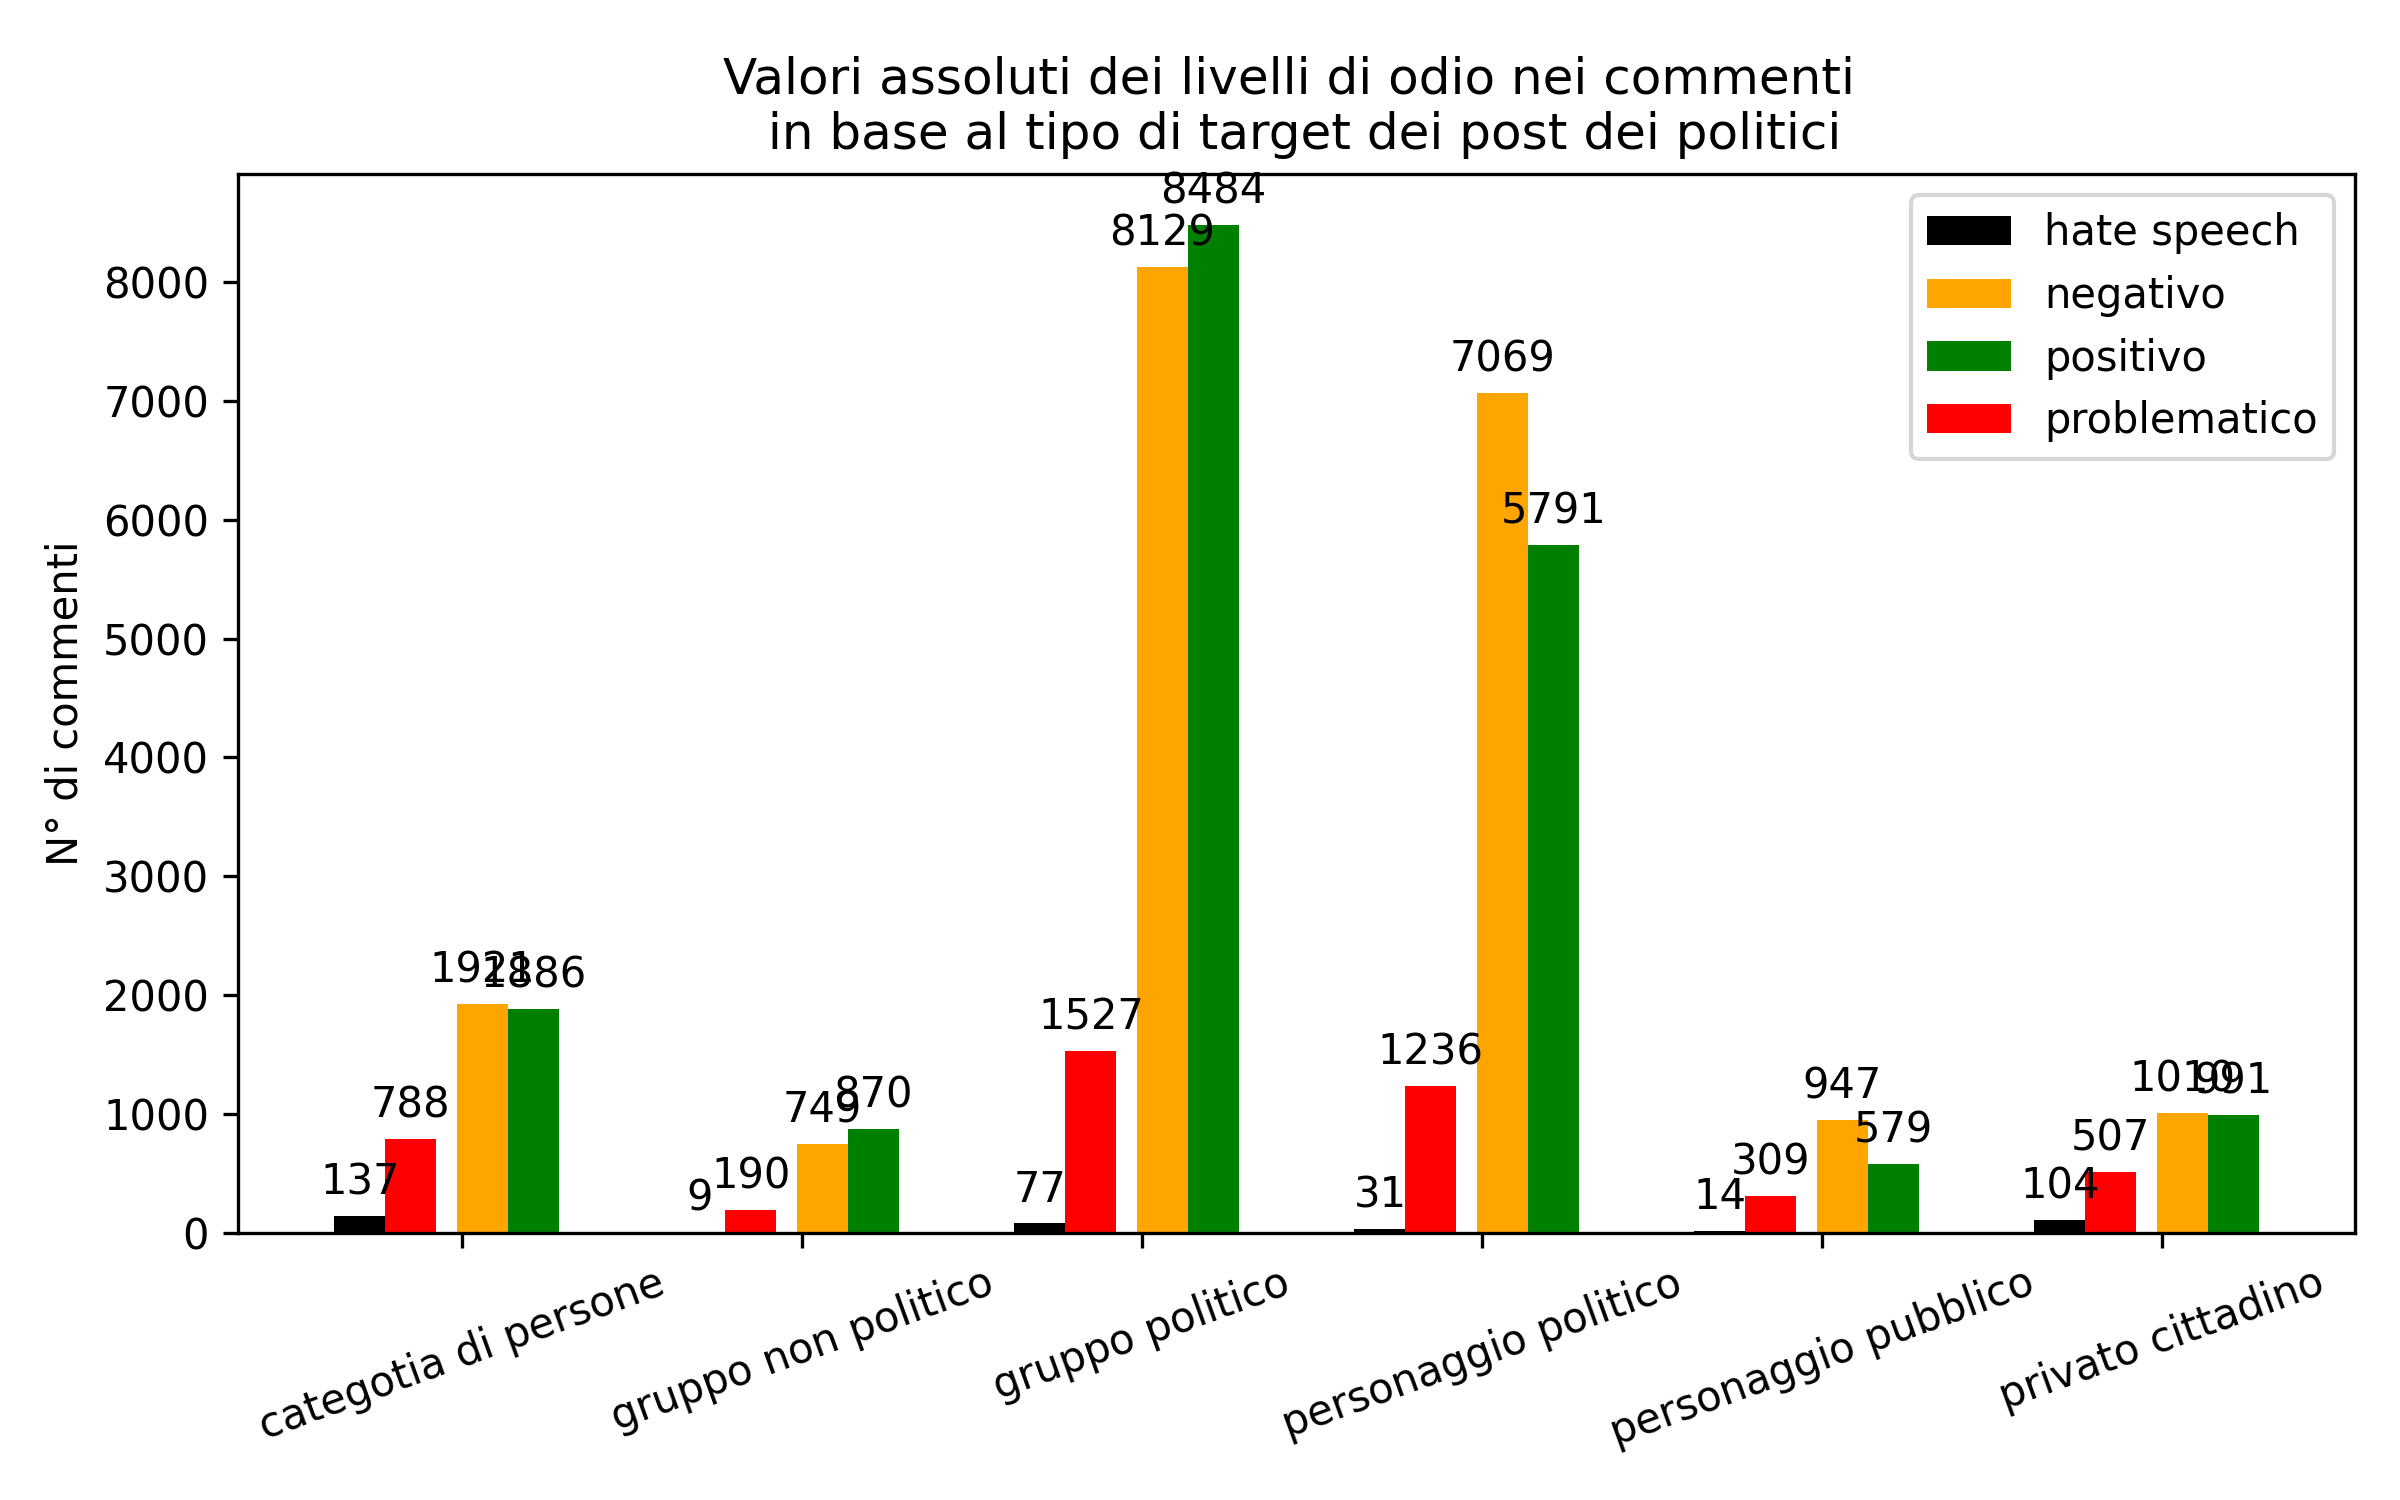
\includegraphics[width=\textwidth]{figures/targetuniq}
	\caption{Valori assoluti dei tipi di commenti in base al target dei post comparativi o negativi a cui rispondono}
	\label{fig:targetuniq}
\end{figure}

Dai valori assoluti [Fig.\ref{fig:targetuniq}] possiamo vedere come la maggior parte dei commenti di \textit{hate speech} siano stati riscontrati in risposta a target riferiti a “categorie di persone” e “privati cittadini”. Benché “Gruppi politici” e “personaggio politico” facciano rilevare molti commenti positivi e negativi senza uso di linguaggio incivile, quando si fa riferimento a “personaggi politici” il numero di commenti negativi è superiore a quello dei commenti positivi. Stesso discorso vale per i “personaggi pubblici” (es. Roberto Saviano) che generano pochi commenti positivi rispetto ai negativi.


Andando ad analizzare la rilevanza dei vari tipi di commento in percentuale sul totale delle risposte ai target [Fig.\ref{fig:targetuniqpercent}], possiamo osservare ancora più chiaramente come i due target non politici e non pubblici (“ categoria di persone” e “privato cittadino”) risultino avere rispettivamente circa 6 e 9 volte più commenti di \textit{hate speech} rispetto agli altri target, che hanno invece percentuali simili sotto l'1\%. Anche i commenti problematici sono più frequenti in proporzione ai commenti che rispondono a post con questi target, registrando valori tra il 50\% e il 100\% più alti degli altri. Solamente il citare un personaggio pubblico genera livelli di commenti problematici simili (16,6\%). Sempre quest'ultima categoria di target è quella con la maggiore differenza (20\%) tra commenti negativi e positivi, con la minore percentuale sul totale di commenti positivi tra tutti i gruppi. Anche quando si fa riferimento a un personaggio politico i commenti sono più negativi che positivi, al di là di problematici ed \textit{hate speech}, ma in questo caso la differenza tra positivi e negativi è solo il 10\%.

Dall’analisi, infine, delle percentuali dei vari tipi di commenti sul totale dei contenuti analizzati, e sempre in relazione al target al quale rispondono, emergono indicazioni su come poter ridurre i livelli di odio sul web [Fig.\ref{fig:targetuniqpercent2}]. Evitando di citare “categorie di persone” e “privati cittadini” nei loro attacchi online (rispettivamente 443 e 239 post, il 6\% del totale di tutto quello che è stato postato) i candidati potrebbero ridurre del 55\% per cento il totale dei commenti di hate speech registrati (241 commenti di odio verso minoranze su 436 totali). 682 post di politici valgono 241 commenti di \textit{hate speech}? Pensiamo di no.

In sintesi: quando i politici attaccano “categorie di persone” e “privati cittadini”, si registrano i maggiori livelli di \textit{hate speech}, anche perché la stessa definizione di questo specifico tipo di linguaggio comprende attacchi a minoranze specifiche. Stesso discorso però anche per i commenti incivili in generale (problematici) il che indica che il riferimento polemico a gruppi e persone che vivono al di fuori dall’arena del dibattito pubblico, autorizza comportamenti più aggressivi e più incivili, anche quando non degenerano nell’\textit{hate speech} vero e proprio. E’ come se i commentatori percepissero un maggior livello di impunità quando l’obiettivo polemico è un personaggio sconosciuto ai più. Oppure si potrebbe ipotizzare che questo tipo di attacchi in qualche modo esca già dai limiti della campagna elettorale, entrando in quello dell’attacco fine a se stesso. Si potrebbe anche discutere del fatto che attacchi a categorie come i Rom o migranti, oppure a privati cittadini in seguito ad un arresto o alla partecipazione ad una manifestazione, siano fatti che non dovrebbero essere usati all’interno di messaggi pubblici in campagne elettorali di livello nazionale o addirittura sovranazionale come in questo caso perchè non di interesse pubblico, essendo casi specifici e che non dovrebbero spingere a generalizzazioni di nessun tipo.
Inoltre, attaccare singoli personaggi (politici o in generale pubblici) rispetto a gruppi (politici o pubblici) genera più commenti negativi che positivi. Anche in questo caso, quindi, si potrebbe dire che i livelli di aggressività siano tanto maggiori quanto maggiore è la vulnerabilità del target attaccato. Privati cittadini e categorie di persone indicate in quanto tali hanno infatti pochissime possibilità di rispondere mediaticamente agli insulti ricevuti, dato che non dispongono di canali social con seguito paragonabile a quello dei politici.
Si riscontra inoltre, come il fenomeno dell'odio risulti particolarmente accentuato anche nel caso dei personaggi pubblici, che fanno registrare altri livelli di commenti “problematici”. Anche se è difficile che i commenti in questo caso sfocino in vero e proprio \textit{hate speech} (a causa della definizione che lo delimita), potrebbe risultare dannoso allo svolgimento di una discussione civile indicare persone al di fuori del contesto politico come simboli di un’idea avversa.
\begin{figure}
	\centering
	\begin{minipage}{.5\textwidth}
		\centering
		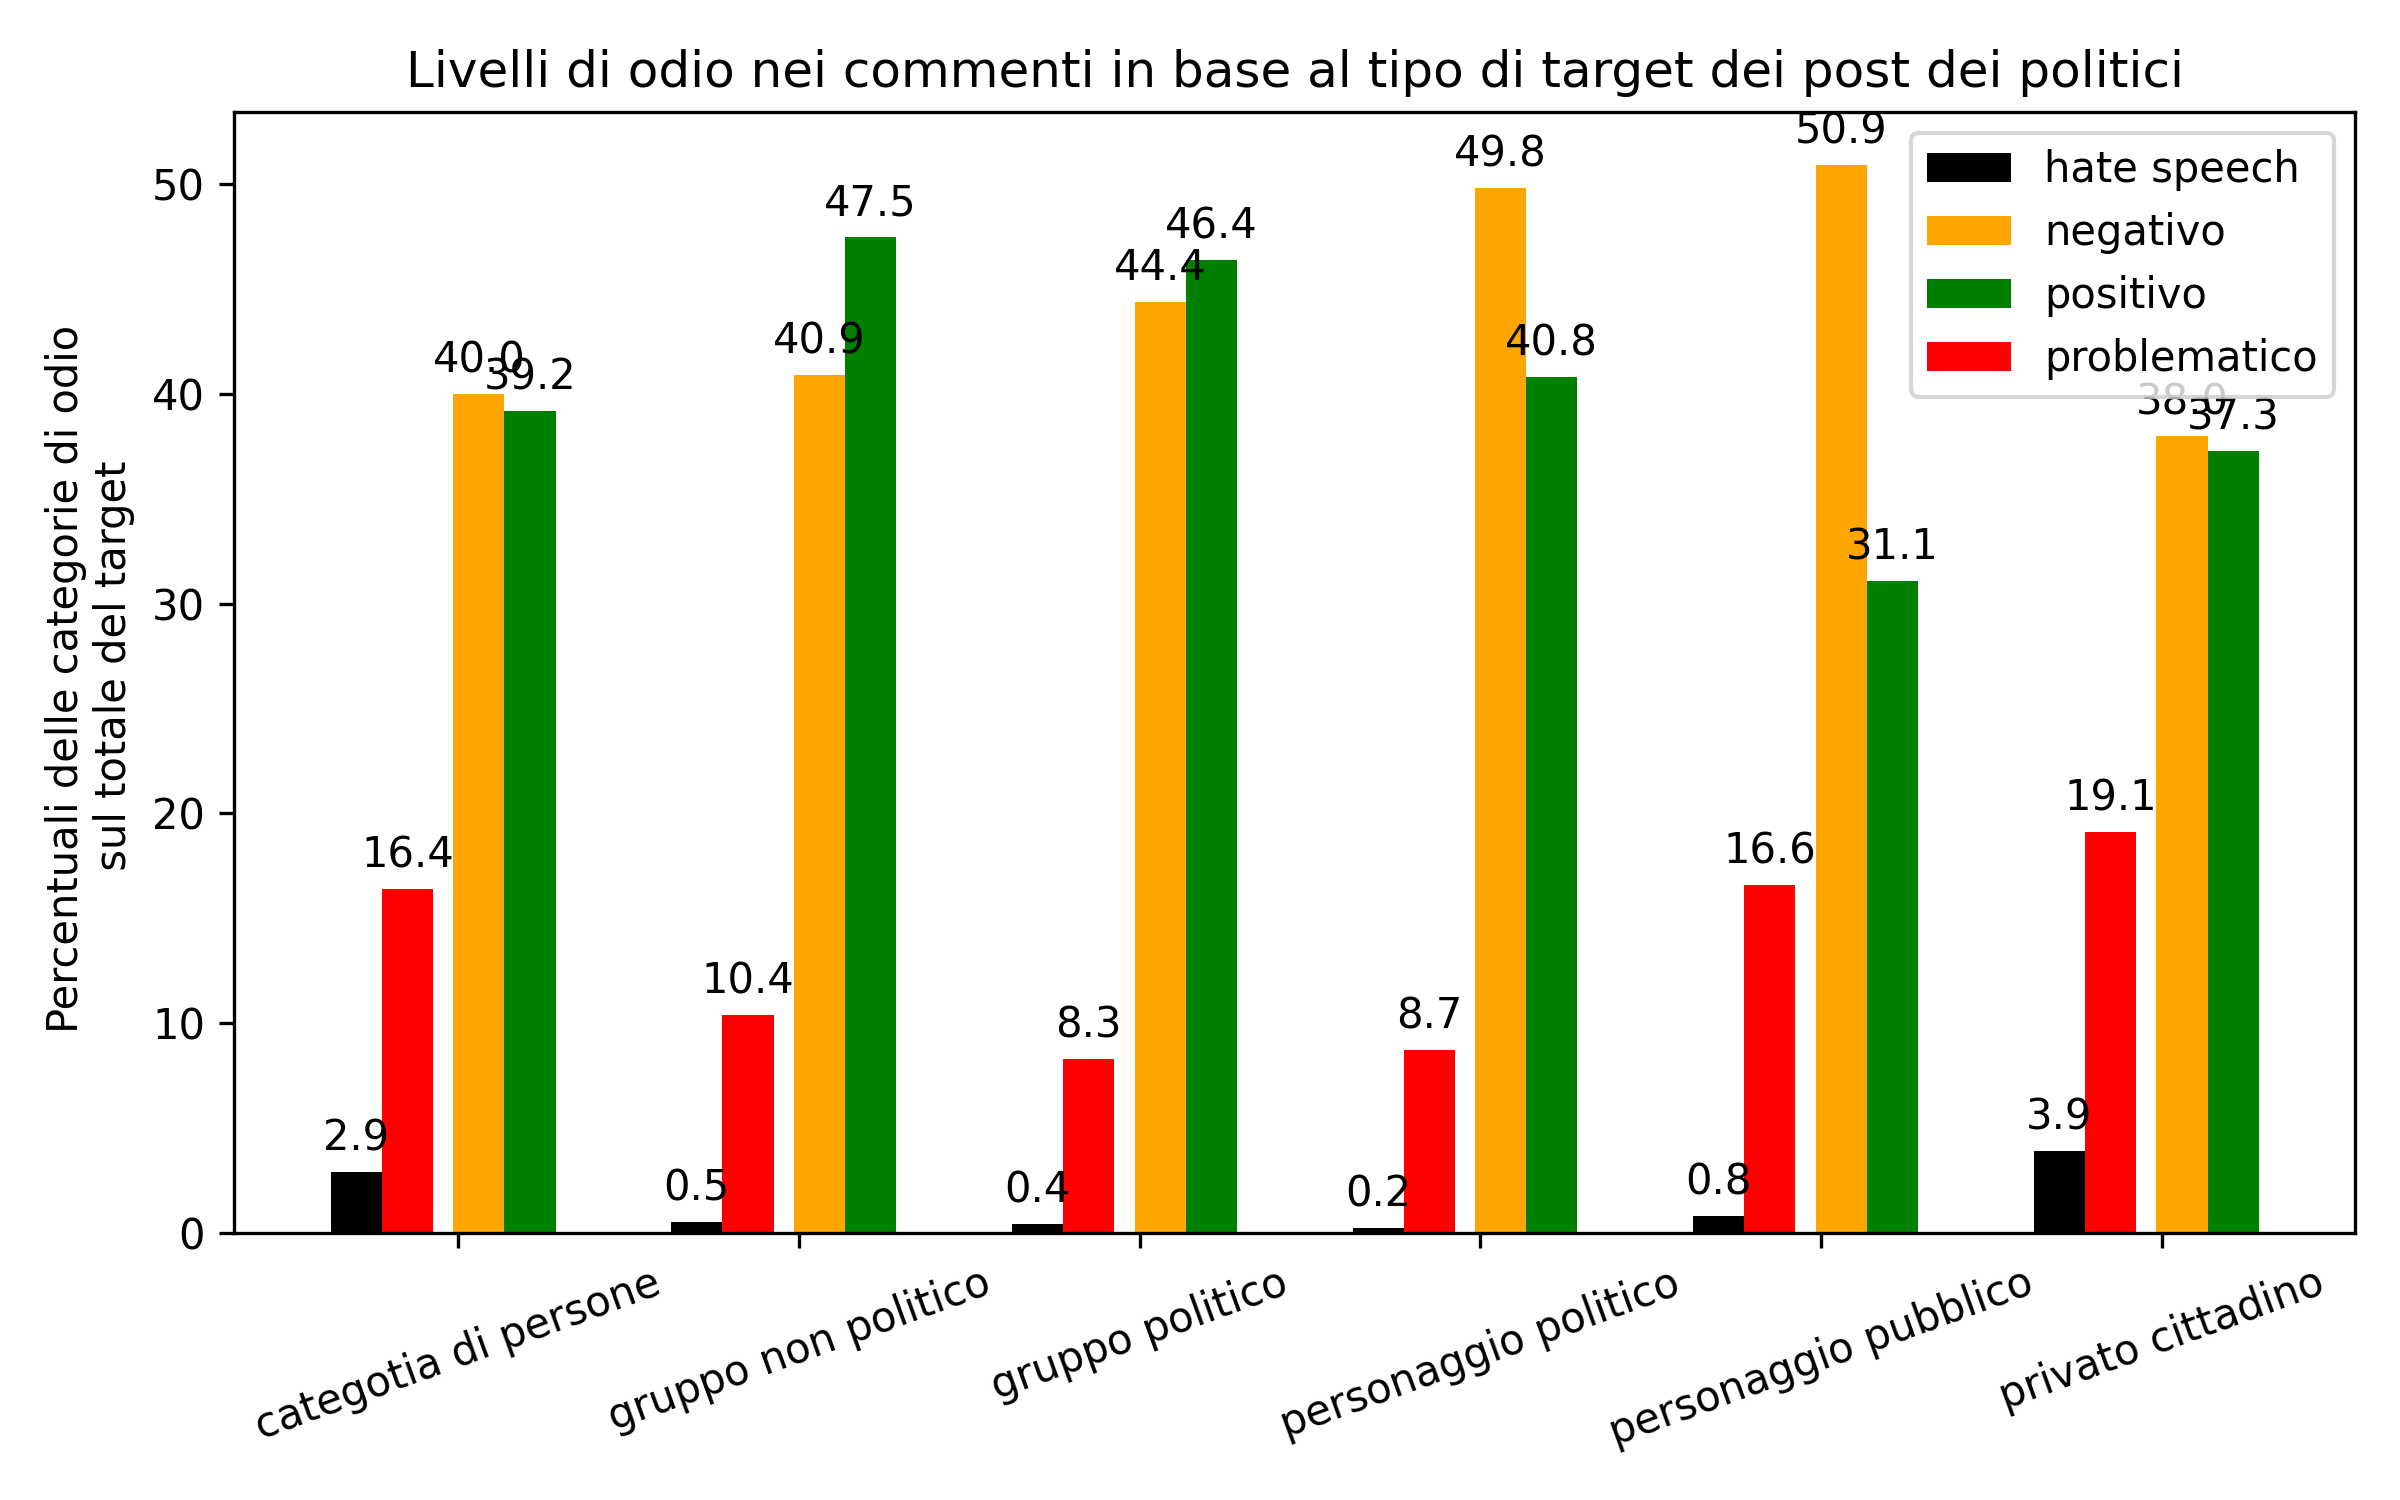
\includegraphics[width=\linewidth]{figures/targetuniqpercent}
		\captionof{figure}{Percentuali dei tipi di commenti sul totale del tipo di target dei post comparativi o negativi a cui rispondono}
		\label{fig:targetuniqpercent}
	\end{minipage}%
	\begin{minipage}{.5\textwidth}
		\centering
		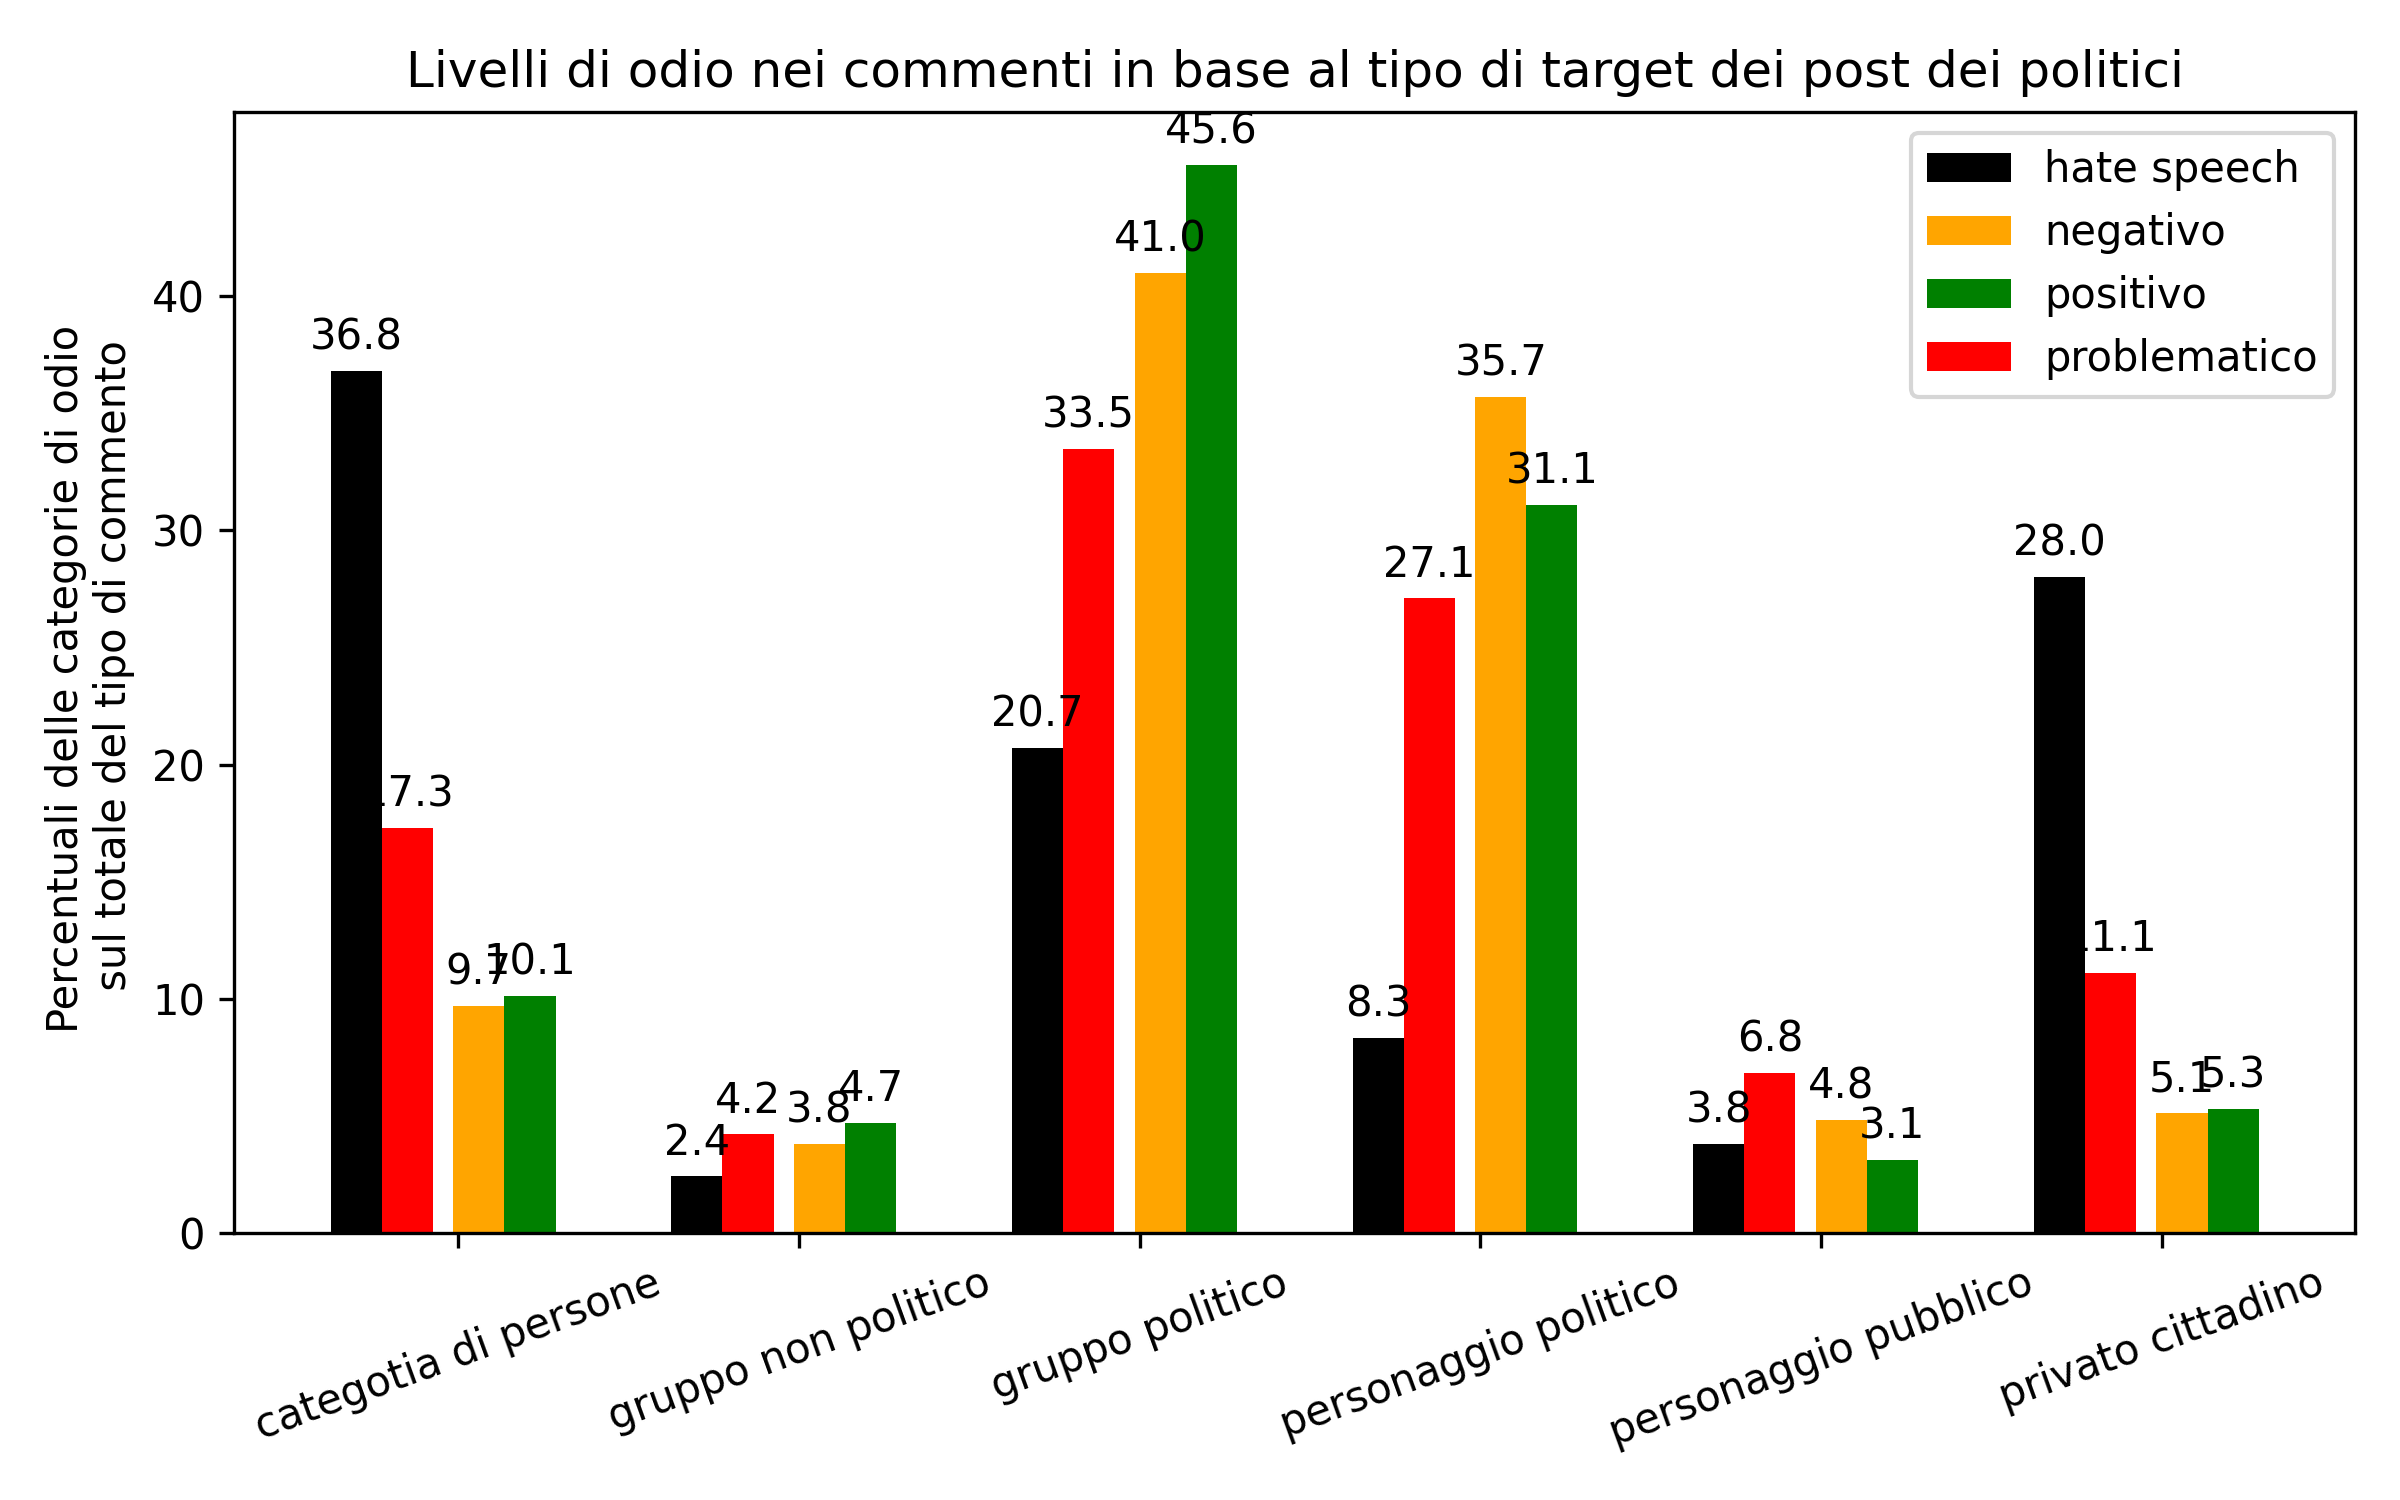
\includegraphics[width=\linewidth]{figures/targetuniqpercent2}
		\captionof{figure}{Percentuali dei tipi di commenti sul totale del tipo di commento in base al target dei post comparativi o negativi a cui rispondono}
		\label{fig:targetuniqpercent2}
	\end{minipage}
\end{figure}

Sembra chiaro quindi che uscire dal contesto pubblico e politico, e coinvolgere nella polemi-ca, gruppi e cittadini sconosciuti ai più,  sia il fattore in grado di generare più odio. Abbiamo riscontrato però anche una prevalenza di messaggi problematici e negativi generati da target singolari rispetto ai corrispettivi plurali. Per vedere se le due ipotesi sono supportate da significatività statistica è stato eseguito un test di chi-quadro.
In questo caso sono stati presi in considerazione tutti i tipi di commenti (anche quelli ambigui) e i target sono stati raggruppati in entrambi i casi in due categorie, riducendo il numero di target totali. Sono stati presi in considerazione anche i target doppi in quanto tali, ma sono stati esclusi dai test quei target doppi che non rientravano in nessuna delle due categorie create per l'analisi.

In  primo luogo, viene testato se vi è una differenza tra i commenti relativi a post comparativi e negativi con target riferito  a personaggi o gruppi di dominio pubblico (“personaggio pubblico e “personaggio politico”, “gruppo politico e gruppo non politico”, più i target doppi che comprendono due di queste categorie) confrontati con quelli che non lo sono (“privato cittadino”, “categoria di persone e privato cittadino” + “categoria di persone”). Gli altri target doppi sono stati eliminati (es. privato cittadino - gruppo politico)[Fig.\ref{fig:pub1}]. Il test ha dato risultati molto significativi con un Pearson chi-square molto altro: $\chi^{2}$ (9, N = 31240) = 879.1844, p = 0.0000. Possiamo quindi dire che quando si fa riferimento a target non di dominio pubblico si crea un significativo aumento di commenti di \textit{hate speech} e problematici nei commenti.
\begin{figure}
	\begin{minipage}{.5\textwidth}
		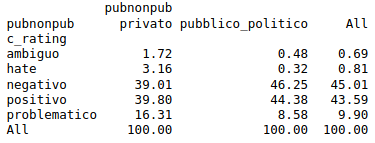
\includegraphics[width=\linewidth]{figures/pub1}
		\captionof{figure}{Percentuali dei tipi di commenti divisi tra quelli che rispondono a un post in cui il target è privato (privato cittadino, categoria di persone) oppure pubblico (personaggio pubblico e politico, gruppo non politico o politico)}
		\label{fig:pub1}
	\end{minipage}
	\begin{minipage}{.5\textwidth}
		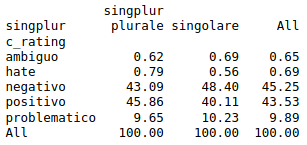
\includegraphics[width=0.85\linewidth]{figures/sing1}
		\captionof{figure}{Percentuali dei tipi di commenti divisi tra quelli che rispondono a un post in cui il target è un singolo (privato cittadino, personaggio pubblico o politico) oppure gruppo (categoria di persone, gruppo non politico o politico)}
		\label{fig:sing1}
	\end{minipage}
\end{figure}

% [Fig.\ref{fig:sing2}]
% [Fig.\ref{fig:pub2}]
%
%\begin{figure}
%    \centering
%%    \begin{minipage}{.5\textwidth}
%%        \centering
%%        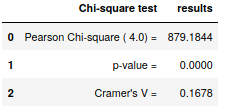
\includegraphics[width=0.9\linewidth]{figures/pub2}
%%        \captionof{figure}{Risultati del test di chi-quadro che verificano la differenza tra i due gruppi: privato VS pubblico}
%%        \label{fig:pub2}
%%    \end{minipage}
%    \begin{minipage}{.5\textwidth}
%        \centering
%        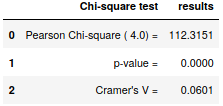
\includegraphics[width=0.9\linewidth]{figures/sing2}
%        \captionof{figure}{Risultati del test di chi-quadro che verificano la differenza tra i due gruppi: singolo VS gruppo}
%        \label{fig:sing2}
%    \end{minipage}
%\end{figure}

Allo stesso modo è stata testata la seconda ipotesi. In questo caso i due gruppi consistono nei target singolari da una parte (“privato cittadino”, “personaggio pubblico e personaggio politico”, più relativi target doppi) e target plurali dall'altra (“categoria di persone”, “gruppo politico” o “gruppo non politico”, più relativi target doppi). Anche in questo caso i target doppi che non rientrano nelle due categorie sono stati esclusi (es. privato cittadino + gruppo politico) [Fig.\ref{fig:sing1}]. I risultati sono significativi anche in questo caso, ma con un effetto minore rispetto al test precedente (9, N = 31083) = 112.3151, p = 0.0000. Possiamo quindi dire che attaccando target singolari rispetto a gruppi si generano commenti più negativi rispetto a quelli positivi, ma non una percentuale maggiore di linguaggi incivili ed \textit{hate speech}. In generale la prima distinzione testata risulta più esplicativa di quest'ultima.



\subsection{Ip.3: i commenti su Twitter sono più negativi?}
Abbiamo visto come il tipo di canale  utilizzato fa cambiare il tipo di comunicazione politica adottata, aumentando la negatività dei messaggi su Twitter rispetto a quelli pubblicati su Facebook. Effetti simili saranno riscontrati anche nella negatività dei commenti?
Analizzando il grafico con le percentuali dei livelli di odio nelle risposte a post e tweet [Fig.\ref{fig:hatefb}], vediamo come in questo caso i risultati siano meno netti e l'ipotesi non risulti del tutto confermata. Se da una parte Facebook registra molti più commenti positivi rispetto a quelli con tono negativo, su Twitter le due percentuali sono praticamente uguali. Sembra quindi che il social di microblogging favorisca commenti più negativi rispetto alla piattaforma di Zuckemberg. Ma quando guardiamo al linguaggio incivile e all’\textit{hate speech}, le proporzioni si invertono. Benché la distribuzione risulti significativamente diversa con un test di $\chi^{2}$ (7, N = 78175) = 1075.1347, p = 0.0000, questa differenza non è chiaramente spiegabile a partire da questo campione e servirebbero altri tipi di dati per poter fare considerazioni più solide. Possiamo ipotizzare che gli odiatori siano più propensi ad utilizzare Facebook rispetto a Twitter, mentre gli/le utenti generici potrebbero essere spinti dal diverso canale comunicativo ad aumentare i loro livelli di negatività, ma le differenze nei tipi di commento che potremmo far risalire agli odiatori sono troppo piccole per poterlo affermare con certezza, e soprattutto non disponiamo di nessuno dato relativo agli/alle utenti dei commenti presi in considerazione, non possiamo quindi paragonare i contenuti nelle due piattaforme per l* stess* utente (come invece abbiamo fatto con i post e tweet dei politici).
\begin{figure}
	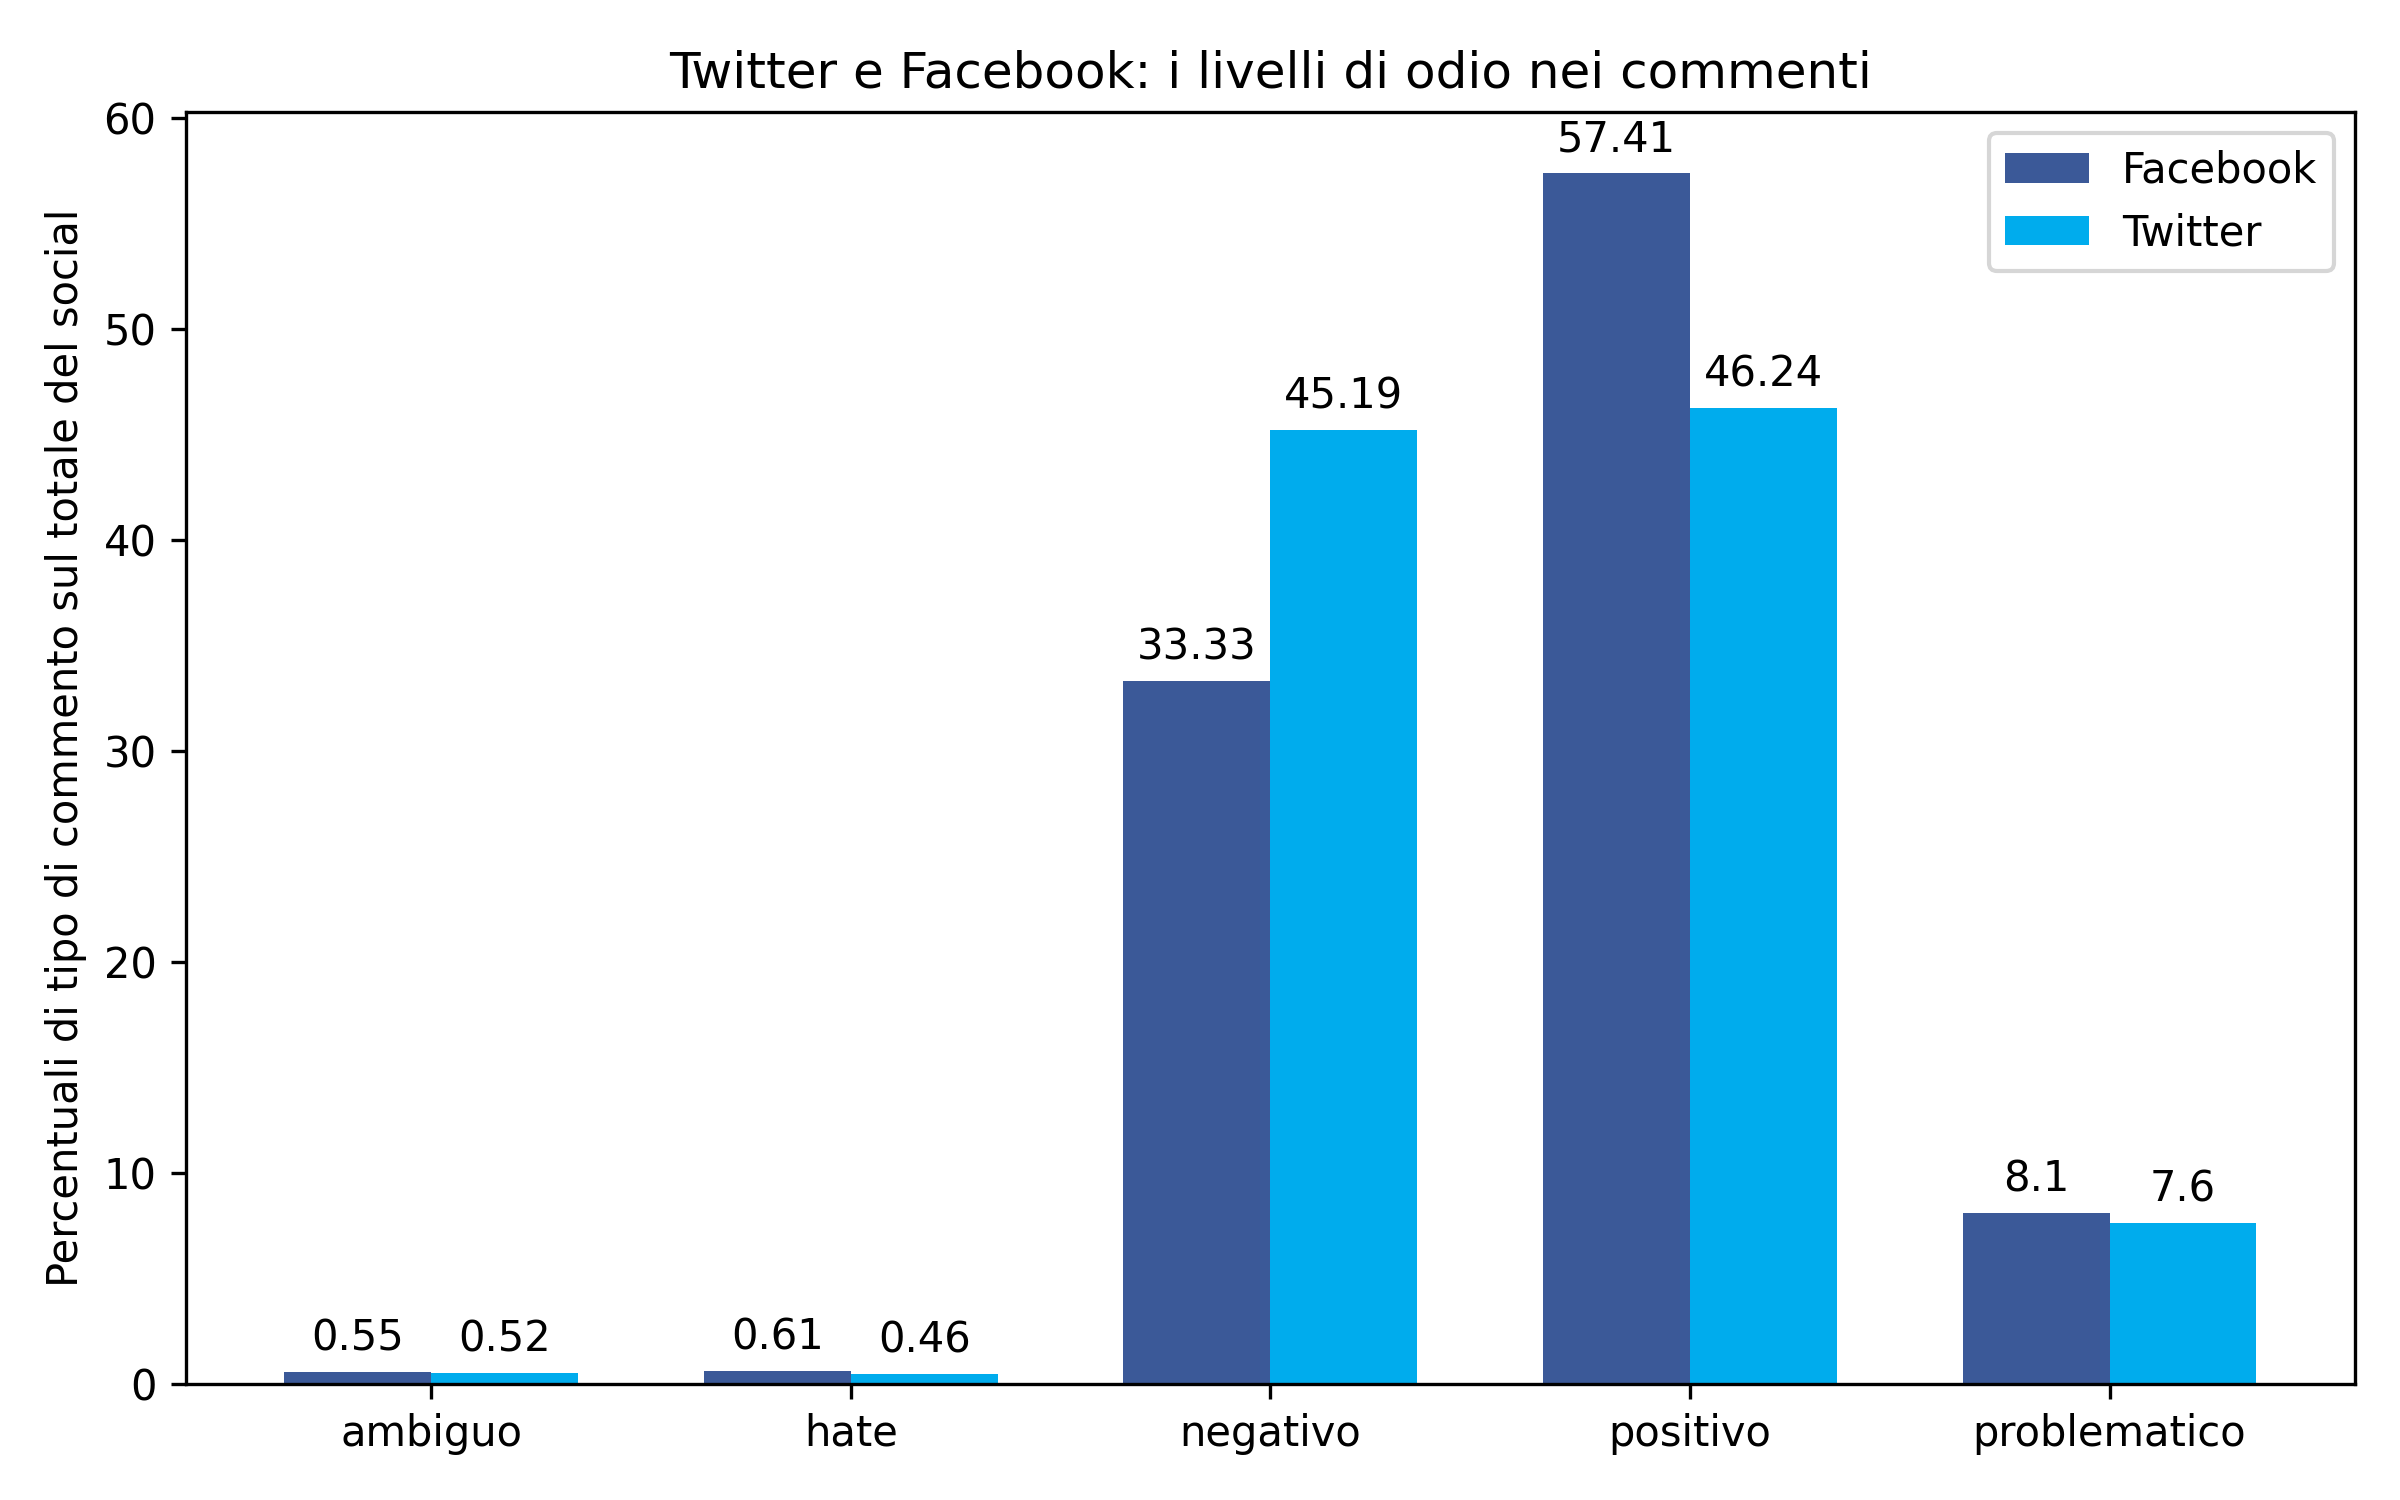
\includegraphics[width=\textwidth]{figures/hatefb}
	\caption{Le percentuali dei vari tipi di commenti sul totale dei due social in considerazione }
	\label{fig:hatefb}
\end{figure}


% DA FARE:
% - fare differenza chi quadri per i vari tipi di campagna politica uno alla volta
% - riportare SDV della lunghezza dei testi e fare un GLM 2x2 per diffrenza lunghezza testo
% - mettere le medie

%ARTICOLI CHE NON CI STAVANO:
% 1)libro sul crowsourcing del 2013 https://books.google.it/books?hl=it&lr=&id=ndcnAAAAQBAJ&oi=fnd&pg=PR5&ots=WMwshRMl_g&sig=Mprk85A9d852VnIwykn3_n9Ou2U&redir_esc=y#v=onepage&q&f=false



